% documentclass options:
\documentclass[11pt,DIV=16,
  a4paper,
  parskip=half, % This is some extra vertical space between paragraphs, the suggestion is 2cm which is really ugly, so we use what koma script gives us
  % you can also set it to full for even more space. But there is a bad tex style decision: parskip also changes the spacing between listitems such as
  % enumerate and itemize. For this purpose we include the enumitem package and set itemsep=.5em, of course you can change this
  BCOR=10mm,
  ngerman, % BCOR is binding correction
  % if you'd rather have a one sided thesis, add `oneside' to the documentclass
  % oneside,
  % ngerman is needed for hyphenation if the thesis contains parts written in German, switch order with english if you write mainly in English.
  % Remember to change order in the babel package (below) as well.
  % Last language is the preferred one.
  english]{scrbook}
\usepackage[ngerman,english]{babel} % If you write mainly in English change order to ngerman, english. Also change that in the documentclass options above.
% Include of titling must happen before \title etc.
% that's why it's not in setup.tex
\usepackage{titling}
\title{Using $Z\to\tau\tau$ events to calculate tau ID scale factors using high $p_T$ tau leptons}
\author{Diego Baron}

% Change to your first examiner
% The ~ enables non sentence spacing after a period
\newcommand{\advisers}{Prof. Terry Wyatt}
\newcommand{\firstexaminer}{Dr. Marco Gersabeck}
% Change to your second examiner, some undergraduate studies don't have a second examiner
% in this case just comment out the following line
%\newcommand{\secondexaminer}{Prof.~Dr.~Wile E. Coyote}
% Change to your adivers
% include all packages and define commands in setup.tex

%------------------------------------------------------------------------------
%       package includes
%------------------------------------------------------------------------------
    % font encoding is set up for pdflatex, for other environments see
    % http://tex.stackexchange.com/questions/44694/fontenc-vs-inputenc
    \usepackage[T1]{fontenc}  % 8-bit fonts, improves handling of hyphenations
    \usepackage{lmodern}
    \usepackage[utf8]{inputenc}
    \usepackage{slashed}
    % provides `old' commands for table of contents. Eases the ability to switch
    % between book and scrbook
    \usepackage{scrhack}
    \newcommand{\nn}{\nonumber}
    \newcommand{\taul}{\tau_\text{lep}}
    \newcommand{\tauh}{\tau_\text{h}}
    \newcommand{\pt}{p_\text{T}}
    \newcommand{\ptmiss}{\slashed{E}_T}
    \newcommand{\mreco}{m_{\text{reco}}}
    \usepackage[english]{babel}
	\usepackage[style=numeric, sorting=none,,backend=biber]{biblatex}
	\addbibresource{bib/topic1.bib}
    % ------------------- layout, default -------------------
    % adjust the style of float's captions, separated from text to improve readabilty
    \usepackage[labelfont=bf, labelsep=colon, format=hang, textfont=singlespacing]{caption}
    % With format = hang your caption will look like this:
    % Figure 1: Lorem ipsum dolor sit amet,
    %           consectetuer adipiscing elit.
    %           Ut purus elit, vestibulum
    % If you instead want
    % Figure 1: Lorem ipsum dolor sit amet,
    % consectetuer adipiscing elit. Ut purus
    % elit, vestibulum
    % change to format=plain
    \usepackage{chngcntr}  % continuous numbering of figures/tables over chapters
    \counterwithout{equation}{chapter}
    \counterwithout{figure}{chapter}
    \counterwithout{table}{chapter}

    % Uncomment the following line if you switch from scrbook to book
    % and comment the setkomafont line
    \usepackage{titlesec}  % remove "Chapter" from the chapter title
    \titleformat{\chapter}[hang]{\bfseries\huge}{\thechapter}{2pc}{\huge}
    \titlespacing*{\chapter}{0pt}{10pt}{10pt}
    %\setkomafont{chapter}{\normalfont\bfseries\huge}
        \makeatletter
    \renewcommand\chapter{\par%
    	\thispagestyle{plain}%
    	\global\@topnum\z@
    	\@afterindentfalse
    	\secdef\@chapter\@schapter}
    \makeatother

    \usepackage{setspace}  % Line spacing
    \onehalfspacing
    % \doublespacing  % uncomment for double spacing, e.g. for annotations in correction

    % ------------------- functional, default-------------------
    \usepackage[dvipsnames]{xcolor}  % more colors
    \usepackage{array}  % custom format per column in table - needed on the title page
    \usepackage{graphicx}  % include graphics
    \usepackage{subcaption}  % divide figure, e.g. 1(a), 1(b)...
    \usepackage{amsmath}  % |
    \usepackage{amsthm}   % | math, bmatrix etc
    \usepackage{amsfonts} % |
    \usepackage{calc}  % calculate within LaTeX
    \usepackage[unicode=true,bookmarks=true,bookmarksnumbered=true,
                bookmarksopen=true,bookmarksopenlevel=1,breaklinks=false,
                pdfborder={0 0 0},backref=false,colorlinks=false]{hyperref}
                
    \usepackage{etoolbox} % if-else commands
    %==========================================
    % You might not need the following packages, I only included them as they
    % are needed for the example floats
    % ------------------- functional, custom -------------------
    \usepackage{algorithm,algpseudocode}
    \usepackage{bm}  % bold greek variables (boldmath)
    \usepackage{tikz}
    \usetikzlibrary{positioning}  % use: above left of, etc
    
    % required for the ToDo list
    \usepackage{ifthen}

    % Improves general appearance of the text
    \usepackage[protrusion=true,expansion=true, kerning]{microtype}
    \usepackage{enumitem}
    % nicer font for pdf rendering
    %\usepackage{lmodern}
    
    % For nicer looking tables
    \usepackage{booktabs}

    % usually you don't need this, just for demonstration of a longer caption
    \usepackage{lipsum}

%------------------------------------------------------------------------------
%       (re)new commands / settings
%------------------------------------------------------------------------------
    % ----------------- referencing ----------------
    \newcommand{\secref}[1]{Section~\ref{#1}}
    \newcommand{\chapref}[1]{Chapter~\ref{#1}}
    \renewcommand{\eqref}[1]{Eq.(\ref{#1})}
    \newcommand{\figref}[1]{Figure~\ref{#1}}
    \newcommand{\tabref}[1]{Table~\ref{#1}}

    % ------------------- colors -------------------
    \definecolor{darkgreen}{rgb}{0.0, 0.5, 0.0}
    % Colors of the Albert Ludwigs University as in
    % https://www.zuv.uni-freiburg.de/service/cd/cd-manual/farbwelt
    \definecolor{UniBlue}{RGB}{0, 74, 153}
    \definecolor{UniRed}{RGB}{193, 0, 42}
    \definecolor{UniGrey}{RGB}{154, 155, 156}


    % ------------------- layout -------------------
    % prevents floating objects from being placed ahead of their section
    \let\mySection\section\renewcommand{\section}{\suppressfloats[t]\mySection}
    \let\mySubSection\subsection\renewcommand{\subsection}{\suppressfloats[t]\mySubSection}



    % ------------------- math formatting commands -------------------
    % define vectors to be bold instead of using an arrow
    %\renewcommand{\vec}[1]{\mathbf{#1}}
    \newcommand{\mat}[1]{\mathbf{#1}}
    % tag equation with name
    \newcommand{\eqname}[1]{\tag*{#1}}


    % ------------------- pdf settings -------------------
    % ADAPT THIS
    \hypersetup{pdftitle={\thetitle},
                pdfauthor={\theauthor},
                pdfsubject={Undergraduate thesis at the Albert Ludwig University of Freiburg},
                pdfkeywords={deep learning, awesome algorithm,  undergraduate thesis},
                pdfpagelayout=OneColumn, pdfnewwindow=true, pdfstartview=XYZ, plainpages=false}


    %==========================================
    % You might not need the following commands, I only included them as they
    % are needed for the example floats

    % ------------------- Tikz styles -------------------
    \tikzset{>=latex}  % arrow style


    % ------------------- algorithm ---------------------
    % Command to align comments in algorithm
    \newcommand{\alignedComment}[1]{\Comment{\parbox[t]{.35\linewidth}{#1}}}
    % define a foreach command in algorithms
    \algnewcommand\algorithmicforeach{\textbf{foreach}}
    \algdef{S}[FOR]{ForEach}[1]{\algorithmicforeach\ #1\ \algorithmicdo}

    % line spacing should be 1.5
    \renewcommand{\baselinestretch}{1.2}

    % set distance between items in a list, for more details see the
    % enumitem package: https://www.ctan.org/pkg/enumitem
    \setlist{itemsep=.5em}
    
    % use ra in your tables to increase the space between rows
    % 1.3 should be fine
    \newcommand{\ra}[1]{\renewcommand{\arraystretch}{#1}}

	% ToDo counters
	\usepackage{ifthen} %für whiledo-Schleife
	\newcounter{todos}
	\setcounter{todos}{0}
	\newcounter{extends}
	\setcounter{extends}{0}
	\newcounter{drafts}
	\setcounter{drafts}{0}

	% ------------------- marker commands -------------------
    % ToDo command
    \newcommand{\todo}[1]{\textbf{\textcolor{red}{(TODO: #1)}}\refstepcounter{todos}\label{todo \thetodos}}
	\newcommand{\extend}[1]{\textbf{\textcolor{darkgreen}{(EXTEND: #1)}}\refstepcounter{extends}\label{extend \theextends}}
	% Lighter color to note down quick drafts
	\newcommand{\draft}[1]{\textbf{\textcolor{NavyBlue}{(DRAFT: #1)}}\refstepcounter{drafts}\label{draft \thedrafts}}
	
	% microtype with lmodern, see https://tex.stackexchange.com/questions/75305/microtype-warning-with-lmodern-package-and-koma-script
	%\DeclareMicrotypeAlias{lmss}{cmr}
\begin{document}
    \pagestyle{empty} % no header and no page number
    % disable hyper links to remove warning "destination with same identifier"
    % this means within this section nothing can be referenced with a hyperlink
    \hypersetup{pageanchor=false}

    % enable/disable, depending on your chosen language
    
\begin{titlepage}
\begin{center}

\newcommand{\HorizontalLine}{\rule{\linewidth}{0.3mm}}

{\Large 1st Year PhD Report}\\[1.3cm]


% _____________________________________________________________________________
\HorizontalLine \\[0.4cm]
% Write your title in a fancy way like this if you want to customize it, otherwise simply let tex do it for you
% \begin{spacing}{3}
%     {\huge \bfseries The Long, Long } \\
%     {\huge \bfseries Long Long} \\
%     {\huge \bfseries Title}\\
% \end{spacing}
{ \huge \bfseries \thetitle }
\HorizontalLine \\[1.5cm]
% _____________________________________________________________________________


{\Huge \theauthor} \\[2cm]


\begin{tabular}[hc]{>{\huge}l >{\huge}l}
  
  Supervisor: & \advisers \\[1.2cm]
  Examiner: & \firstexaminer \\[0.3cm]
\end{tabular}
\vfill  % move the following text to the bottom

\Large {
    University of Manchester\\
    Faculty of Science and Engineering\\
    School of Physics and Astronomy\\

    June, 2020\\
}
\end{center}
\end{titlepage}

\thispagestyle{empty}
% title page back
\ \vfill \ \\  % at least one space required before vfill
\
\textbf{Writing Period}            \smallskip{} \\
01.\,05.\,2020 -- 30.\,06.\,2020   \bigskip{} \\
\
\textbf{Supervisor}                  \smallskip{} \\
\advisers							\smallskip{} \\	
\textbf{Examiner}                  \smallskip{} \\
\firstexaminer                     \bigskip{} \\
\
% If there is a second examiner include it
\ifdef{\secondexaminer}
	{
	% Include
	\textbf{Second Examiner}       \smallskip{} \\
	\secondexaminer                \bigskip{} \\
	\
	}
	{
	% No second examiner, ignore
	}

    %\begin{titlepage}
\begin{center}

\newcommand{\HorizontalLine}{\rule{\linewidth}{0.3mm}}

{\Large 1st year PhD Report}\\[1.3cm]


% _____________________________________________________________________________
\HorizontalLine \\[0.4cm]
% Write yourtitle in a fancy way like this if you want to customize it, otherwise simply let tex do it for you
% \begin{spacing}{3}
%     {\huge \bfseries Der Lange, Lange } \\
%     {\huge \bfseries Lange Lange} \\
%     {\huge \bfseries Titel}\\
% \end{spacing}
{ \huge \bfseries \thetitle }
\HorizontalLine \\[1.5cm]
% _____________________________________________________________________________


{\Huge \theauthor} \\[2cm]


\begin{tabular}[hc]{>{\huge}l >{\huge}l}
  Gutachter: & \firstexaminer \\[0.3cm]
  Betreuer: & \advisers \\[1.2cm]
\end{tabular}
\vfill  % move the following text to the bottom

\Large {
    Albert-Ludwigs-Universität Freiburg\\
    Technische Fakultät\\
    Institut für Informatik\\
    Lehrstuhl für Thesis-Templates\\[1cm]

    3. April 2017
    \\
}
\end{center}
\end{titlepage}

\thispagestyle{empty}
% title page back
\ \vfill \ \\  % at least one space required before vfill
\
\textbf{Bearbeitungszeit}            \smallskip{} \\
05.\,07.\,2016 -- 05.\,10.\,2016   \bigskip{} \\
\
\textbf{Gutachter}                  \smallskip{} \\
\firstexaminer                      \bigskip{} \\
\
% If there is a second examiner include it
\ifdef{\secondexaminer}
	{
	% Include
	\textbf{Zweitgutachter}        \smallskip{} \\
	\secondexaminer                \bigskip{} \\
	\
	}
	{
	% No second examiner, ignore
	}
\textbf{Betreuer}                  \smallskip{} \\
\advisers

    \pagestyle{plain} % remove chapter name from top, page number at the bottom
    % use \pagestyle{headings} for having the chapter on top of the pages
    % if you wang a more fancy header use \usepackage[automark,headsepline]{scrlayer-scrpage}
    % and read about it in the KOMA script documentation, https://www.ctan.org/pkg/koma-script
    \frontmatter  % roman page numbers
    %\input{chapters/0_1-declaration}
    %\chapter*{Abstract}
This report is a review of the work done by the student Diego Baron during his first year in the PhD in particle physics program at the University of Manchester. Thus, it is a work in progress. The tau lepton has life time of the order of picoseconds, thus it decays before it can reach the ATLAS detector. So the indirect observation of the tau is done by measuring its decay products. The tau lepton has enough mass to decay not only into the lighter leptons but into hadrons. The leptonic tau decays at the moment can not be differentiated from prompt leptons. In the case of hadronic tau decays the jets produced have different characteristics that make them distinguishable from QCD initiated jets. Different algorithms have been trained to separate true hadronically decaying taus from QCD jets. The efficiency of these algorithms is compared in simulation and data and correction factors are derived to account for the differences that may arise from the simulation limitations. Our study makes use of $Z\to\tauh l=e,\mu$ events, highly boosted in the transverse plane, to evaluate the performance of the tau-ID algorithms for high-$\pt$ taus.




    \tableofcontents
    \listoffigures
    \listoftables
    %\listofalgorithms
    \hypersetup{pageanchor=true}  % re-enable hyperlinking

    \mainmatter  % Arabic page numbers
    \chapter{Introduction}\label{chap:introduction}
This is a template for an undergraduate or master's thesis.
The first sections are concerned with the template itself. If this is your first
thesis, consider reading \secref{sec:advice}.

Of course, the structure of this
thesis is only an example.
Discuss with your adviser what structure fits best for your thesis.

\section{Template Structure}
\begin{itemize}
    \item To compile the document either run the makefile or run your compiler on the file `thesis\_main.tex'. The included makefile requires latexmk which automatically runs bibtex and recompiles your thesis as often as needed. Also it automatically places all output files (aux, bbl, ...) in the folder `out'. As the pdf also goes in there, the makefile copies the pdf file to the parent folder. There is also a makefile in the chapters folder, to ensure you can also compile from this directory.

    \item The file `setup.tex' includes the packages and defines commands. For more details see \secref{sec:setup}.

    \item Each chapter goes into a separate document, the files can be found in the folder chapters.

    \item The bib folder contains the .bib files, I'd suggest to create multiple bib files for different topics. If you add some or rename the existing ones, don't forget to also change this in thesis\_main.tex. You can then cite as usual~\cite{kingma2014adam, bromley1993siamesesignature,muja2009flann}.

    \item The template is written in a way that eases the switch from scrbook to book class. So if you're not a fan of KOMA you can just replace the documentclass in the main file. The only thing that needs to be changed in setup.tex is the caption styling, see the comments there.
\end{itemize}


\section{setup.tex}\label{sec:setup}
Edit setup.tex according to your needs. The file contains two sections, one for package includes, and one for defining commands. At the end of the includes and commands there is a section that can safely be removed if you don't need algorithms or tikz. Also don't forget to adapt the pdf hypersetup!!\\
setup.tex defines:
\begin{itemize}
    \item some new commands for remembering to do stuff:
    \begin{itemize}
        \item \verb|\todo{Do this!}|: \todo{Do this!}
        \item \verb|\extend{Write more when new results are out!}|:\\ \extend{Write more when new results are out!}
        \item \verb|\draft{Hacky text!}|: \draft{Hacky text!}
    \end{itemize}

    \item some commands for referencing, `in \verb|\chapref{chap:introduction}|' produces 'in \chapref{chap:introduction}'
    \begin{itemize}
        \item \verb|\chapref{}|
        \item \verb|\secref{sec:XY}|
        \item \verb|\eqref{}|
        \item \verb|\figref{}|
        \item \verb|\tabref{}|
    \end{itemize}

    \item the colors of the Uni's corporate design, accessible with\\ \verb|{\color{UniX} Colored Text}|
    \begin{itemize}
        \item {\color{UniBlue}UniBlue}
        \item {\color{UniRed}UniRed}
        \item {\color{UniGrey}UniGrey}
    \end{itemize}

    \item a command for naming matrices \verb|\mat{G}|, $\mat{G}$, and naming vectors \verb|\vec{a}|, $\vec{a}$. This overwrites the default behavior of having an arrow over vectors, sticking to the naming conventions  normal font for scalars, bold-lowercase for vectors, and bold-uppercase for matrices.

    \item named equations:
        \begin{verbatim}
\begin{align}
    d(a,b) &= d(b,a)\\ \eqname{symmetry}
\end{align}
        \end{verbatim}
        \begin{align}
            d(a,b) &= d(b,a)\\ \eqname{symmetry}
        \end{align}
\end{itemize}

\section{Advice}\label{sec:advice}
This section gives some advice how to write a thesis ranging from writing style to formatting. To be sure, ask your advisor about his/her preferences.\\
For a more complete list we recommend to read Donald Knuth's paper on mathematical writing. (At least the first paragraph). \url{http://jmlr.csail.mit.edu/reviewing-papers/knuth_mathematical_writing.pdf}

    \begin{itemize}

        \item If you use formulae pay close attention to be consistent throughout the thesis!

        \item Usually  in a thesis you don't write `In [24] the data is..'. You have more space than a paper has, so write `AuthorXY et al. prepare the data... [24]'. Also pay attention to the placement: The citation is at the end of the sentence before the full stop with a no-break space. \verb|... last word~\cite{XY}.|

        \item Pay attention to comma usage, there is a big difference between English and German. `...the fact that bla...' etc.

        \item Do not write `don't ', `can't' etc. Write `do not', `can not'.

        \item If an equation is at the end of a sentence, add a full stop. If it's not the end, add a comma: {$a= b + c$~~~~(1),}

        \item Avoid footnotes if possible.

        \item Use \verb|``''| for citing, not \verb|""|.

        \item It's important to look for spelling mistakes in your thesis. There are also tools like aspell that can help you find such mistakes.
        This is never an excuse not to properly read your thesis again, but it can help.
        You can find an introduction under \url{https://git.fachschaft.tf/fachschaft/aspell}.

        \item If have things like a graph or any other drawings consider using tikz, if you need function graphs or diagrams consider using pgfplots.
        This has the advantage that the style will be more consistent (same font, formatting options etc.) than when you use some external program.

        \item Discuss with your advisor whether to use passive voice or not. In most computer science papers passive voice is avoided. It's harder to read, more likely to produce errors, and most of the times less precise. Of course there are situations where the passive voice fits but in scientific papers they are rare. Compare the sentence: `We created the wheel to solve this.' to `The wheel was created to solve this', you don't know who did it, making it harder to understand what is your contribution and what is not.
        
        \item In tables avoid vertical lines, keep them clean and neat. See \ref{tab:accuracy} for an example. More details can be found in the `Small Guide to Making Nice Tables' \url{https://www.inf.ethz.ch/personal/markusp/teaching/guides/guide-tables.pdf}

    \end{itemize}

    \chapter{The Standard Model and Lepton Universality Tests}\label{chap2}
This chapter begins with a short description of the Standard Model (SM), followed by a discussion about the Z boson production at the Large Hadron collider. Finally, a review of the tau lepton properties is presented. These include the nature of this particle, its interactions with the other SM particles, its main decay modes and the physics implications of the so called Lepton Universality (LU), one of the SM predictions.  
\section{The Standard Model}\label{chap2secm1}
The Standard Model (SM) is a theory about the fundamental constituents of matter and the interactions between them. Four fundamental interactions are known: gravitational, electromagnetic, weak and strong interactions. The SM is based on the framework of Quantum Field Theory (QFT), in which particles are classified as \textit{bosons} or \textit{fermions}, which correspond to particles with integer and half-integer spin respectively. Fermions form matter and they can interact with each other via the exchange of bosons, which are the force carriers. Three fundamental forces are described by the SM. The strong interaction is explained by a theory called quantum chromodynamics (QCD) \cite{GellMann:1964nj} which relies on the principle of gauge invariance under the $\text{SU(3)}_c$ group. The force carriers of the QCD are called \textit{gluons}. The electromagnetic and weak interactions are unified in the SM and this theory is known as the electroweak (EW) theory \cite{Glashow:1967rx,Salam:1968rm,Weinberg:1967tq}. In this sector of the SM the fields are invariant under $\text{SU(2)}_L\times\text{U(1)}_Y$ group. The force carriers of the electroweak interactions are the $\text{Z}^0,\text{W}^\pm$ bosons and the \textit{photon} ($\gamma$). The gravitational interaction is not described by the SM.
	
Fermions in the SM are classified into \textit{quarks} and \textit{leptons} where the latter do not feel the strong interaction. There are six quarks grouped into three generations with increasing masses. Thus, the heavier generations can decay into the lighter ones. There are also six leptons grouped in three generations. Each generation is heavier than the previous one. There are three charged leptons: the electron ($e$), the muon ($\mu$) and the tau ($\tau$); and their associated neutral partners, the \textit{neutrinos} ($\nu$). In order to give mass to the SM particles the Higgs mechanism was proposed in the 60's \cite{PhysRevLett.13.508,PhysRevLett.13.321,PhysRevLett.13.585}. The existence of the Higgs boson is a further consequence of the Higgs mechanism. The Higgs boson is the only spin-0 particle in the SM. Fig.\ref{Fig14} shows the SM particle content.
\begin{figure}[h]
	\centering
	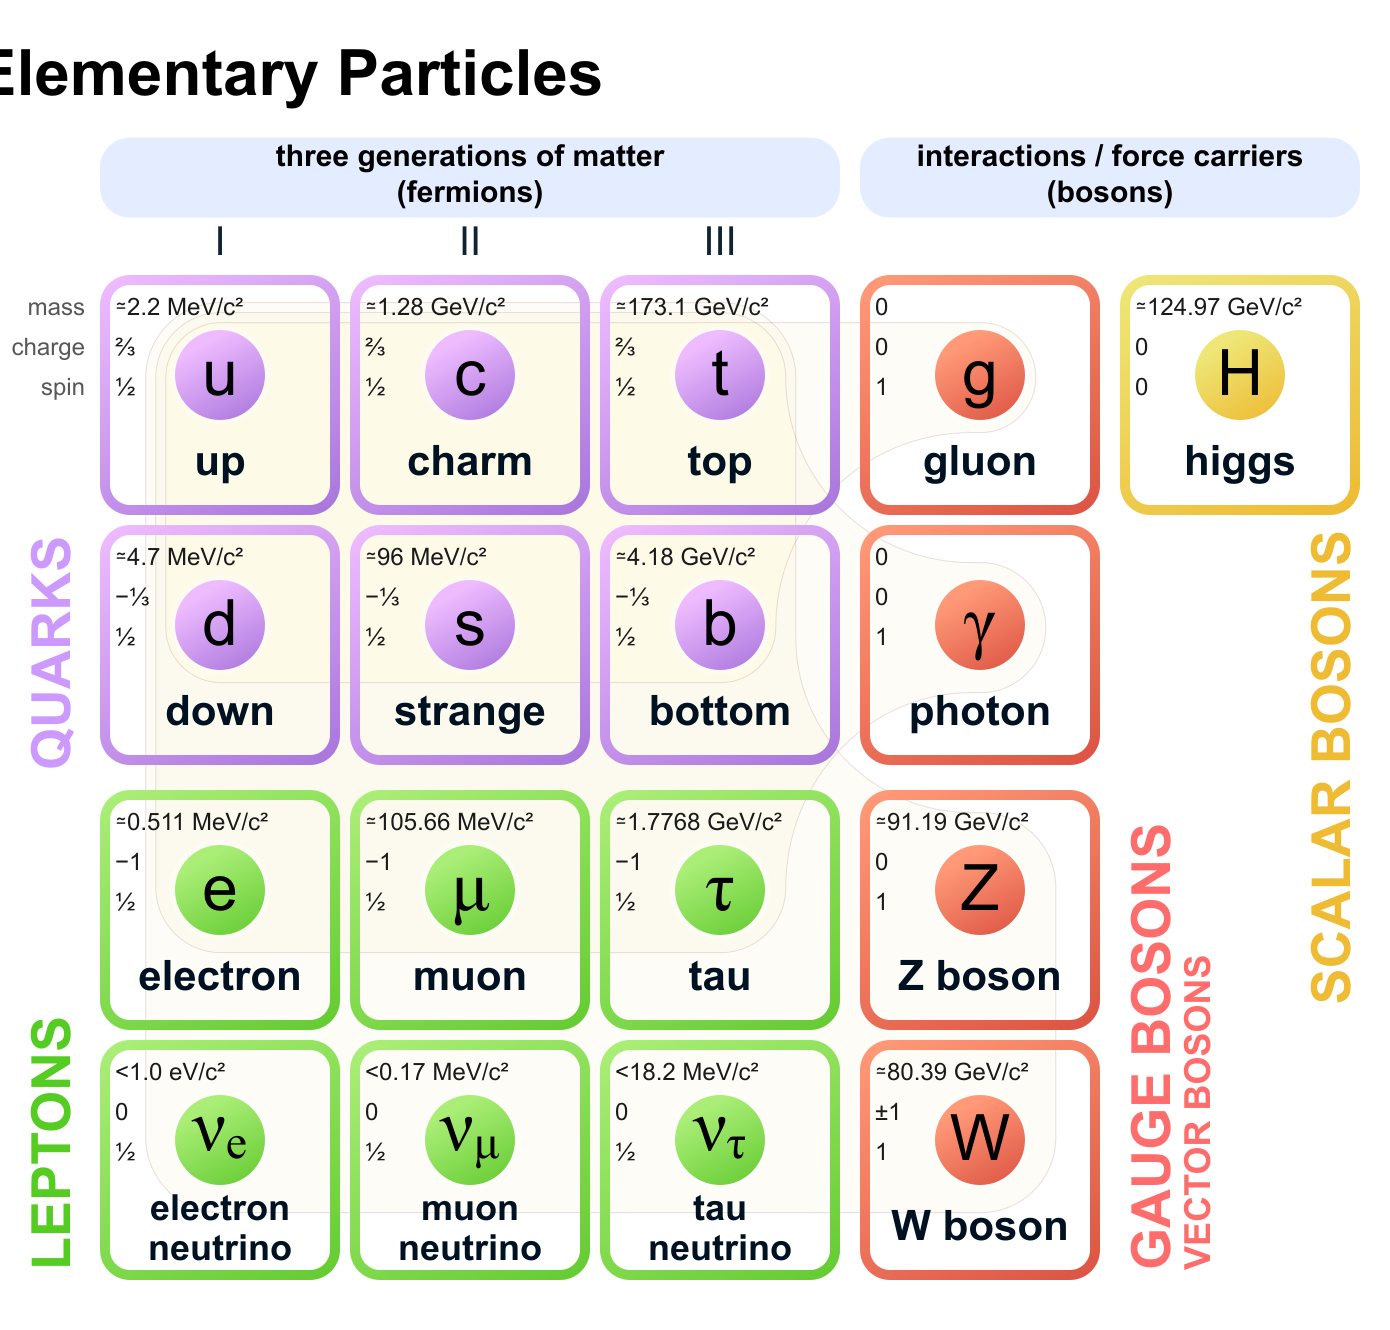
\includegraphics[width=0.7\textwidth]{figures/Fig14}
	\caption{The particle content of the Standard Model. Taken from \cite{SMImage}.}
	\label{Fig14}
\end{figure}
\section{Z boson production at the LHC}\label{chap2sec0}
Since the discovery of the Z and W bosons at the UA1 and UA2 experiments \cite{Arnison:1983rp,Arnison:1983mk,Banner:1983jy,Bagnaia:1983zx}, the Z boson has been the subject of multiple measurements in proton-proton and electron-positron colliders. The Z boson mass $m_Z=91.1875\pm0.0021$ GeV and its decay width $\Gamma_Z=2.4952\pm0.0023$ GeV have been measured to outstanding precision \cite{ALEPH:2005ab}. The braching ratios of the Z boson are well known; they are presented in Table \ref{Table0}.
\begin{table}[]
	\centering
	\begin{tabular}{cc}
		\hline
		\multicolumn{1}{|c|}{Decay mode} & \multicolumn{1}{c|}{Branching fraction (\%)} \\ \hline
		$e^+e^-$                         & $3.363\pm0.004$                              \\
		$\mu^+\mu^-$                     & $3.366\pm0.007$                              \\
		$\tau^+\tau^-$                   & $3.370\pm0.008$                              \\
		Invisible                        & $20.00\pm0.06$                               \\
		Hadrons                          & $69.91\pm0.06$                               \\ \hline
	\end{tabular}
	\caption{Z boson branching fractions. Number taken from \cite{PhysRevD.98.030001}.}
	\label{Table0}
\end{table}
In contrast to electron-positron colliders, the momentum of partons in proton-proton collisions is not precisely known. Thus, parton density functions (PDFs) are used to describe the proton structure in a phenomenological way. These functions are written as $f_{a/A}(x,Q^2)$ and represent the probability density for a parton $a$ to have a fraction $x=\frac{p_a}{p_A}$ of the proton momentum $p_A$. $Q$ is the energy scale of the scattering process. In this case, the cross section of two protons going to a final state $n$ will be
\begin{equation}
	\sigma_{p_Ap_B\to n}=\sum_{q}\int dx_adx_b f_{a/A}(x_a,Q^2) f_{b/B}(x_b,Q^2)\times [\sigma_0+\alpha_s\sigma_1+\dots]_{ab\to n}.
\end{equation}
The sum is made over all the partons. $\sigma_0$ is the tree level parton-parton cross section and $\sigma_1$ are the QCD corrections to first order. A diagram of the production of the Z boson in proton-proton collisions is shown in Fig.\ref{Fig15}. 
\begin{figure}[h]
	\centering
	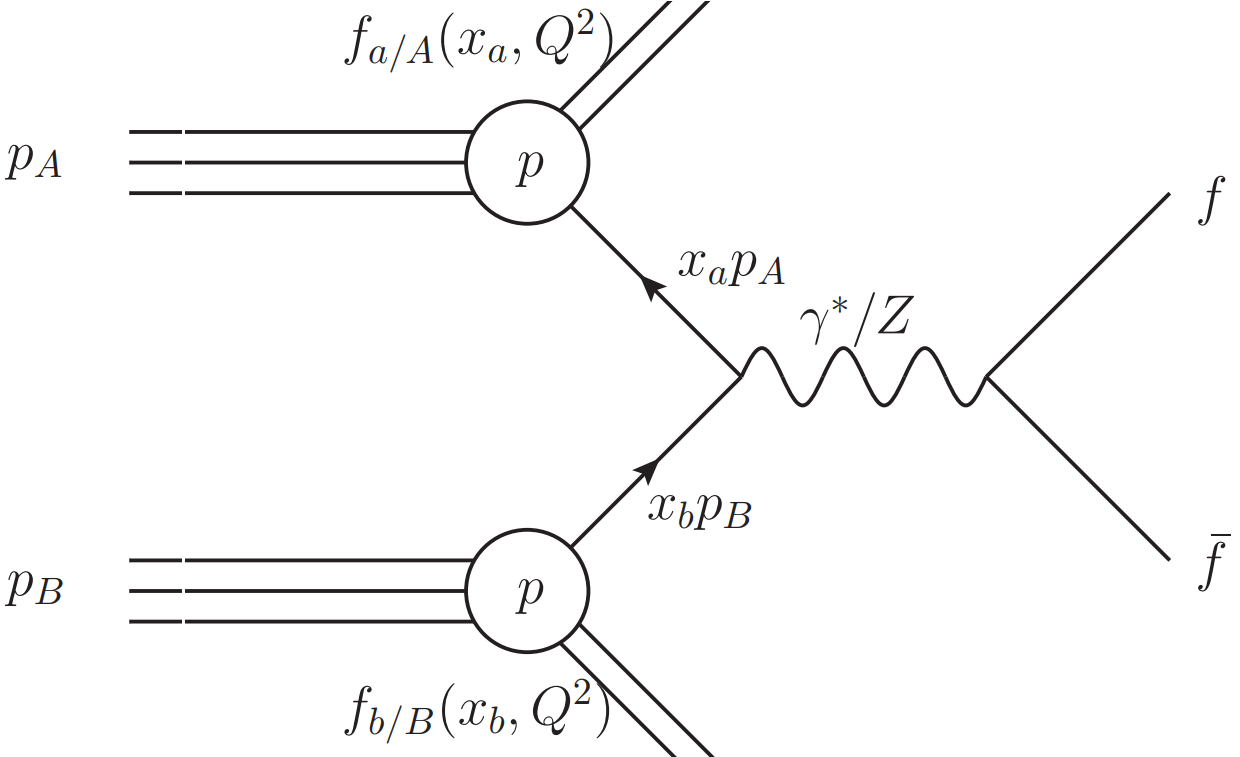
\includegraphics[width=0.6\textwidth]{figures/Fig15}
	\caption{Illustration of the production of a Z boson in pp collisions via quark-antiquark annihilation.}
	\label{Fig15}
\end{figure}
The main process contributing to Z boson production is the Drell-Yan process, where a quark-antiquark ($q\bar{q}$) pair annihilate, produce a Z boson and it subsequently decays into a pair of fermions. In this case, the transverse momentum ($\pt$) of the Z boson comes from the intrinsic $\pt$ of the partons. Nevertheless, this has been experimentally determined with a value of $<k_T>=0.76$ GeV \cite{Ellis:1991qj} and is not large enough to explain the measured Z boson $\pt$ distribution that peaks at a few GeV and has a tail that extends at values $\pt\gg m_Z$ \cite{Abbott:1999yd,Affolder:1999jh}.

To explain this kinematic feature we have to look at the other ways the Z boson can be produced in $pp$ collisions. First quark-gluon ($qg$) scattering, where the Z boson recoils against the quark radiated by the gluon in the initial state, this process is illustrated in Fig.\ref{Fig16a}. In the other hand, we could also have a gluon being radiated before $q\bar{q}$ annihilation takes place, having the Z boson recoiling against what is called \textit{initial state radiation} (ISR), as is shown in Fig.\ref{Fig16b}. High transverse momentum partons lead to the production of collimated showers of hadrons, called jets, that are subsequently detected as energy deposits in the calorimeters of the particle detectors. 
\begin{figure}[ht]
	\centering
	\subfloat[]{\label{Fig16a}{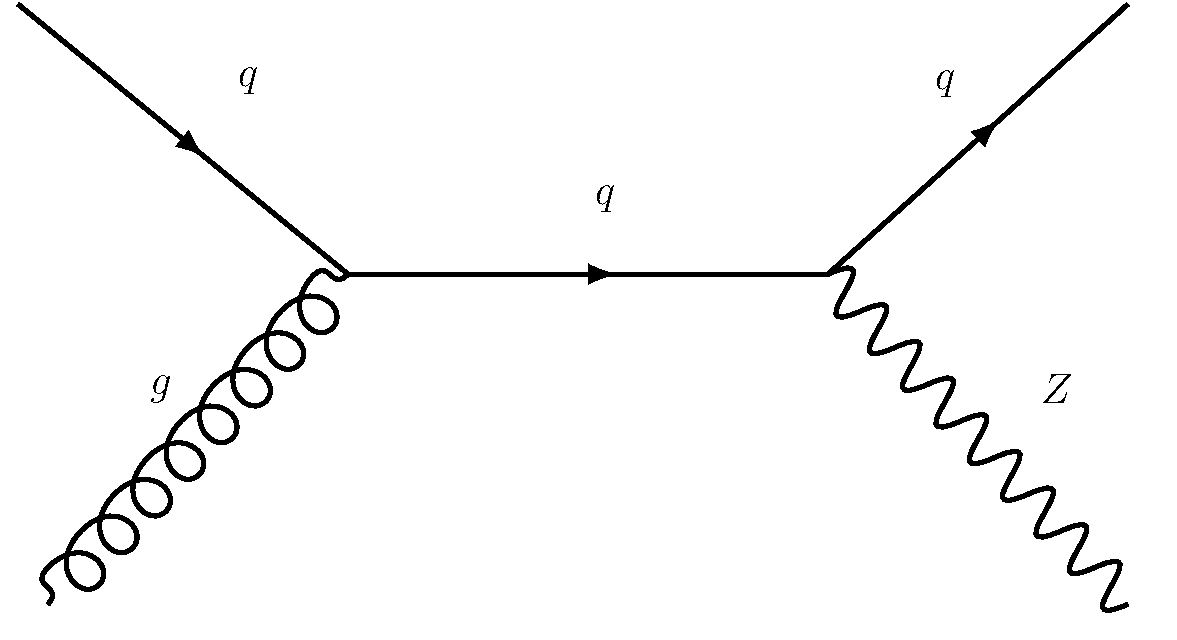
\includegraphics[width=0.50\textwidth]{figures/Fig16a}}}\hfill
	\subfloat[]{\label{Fig16b}{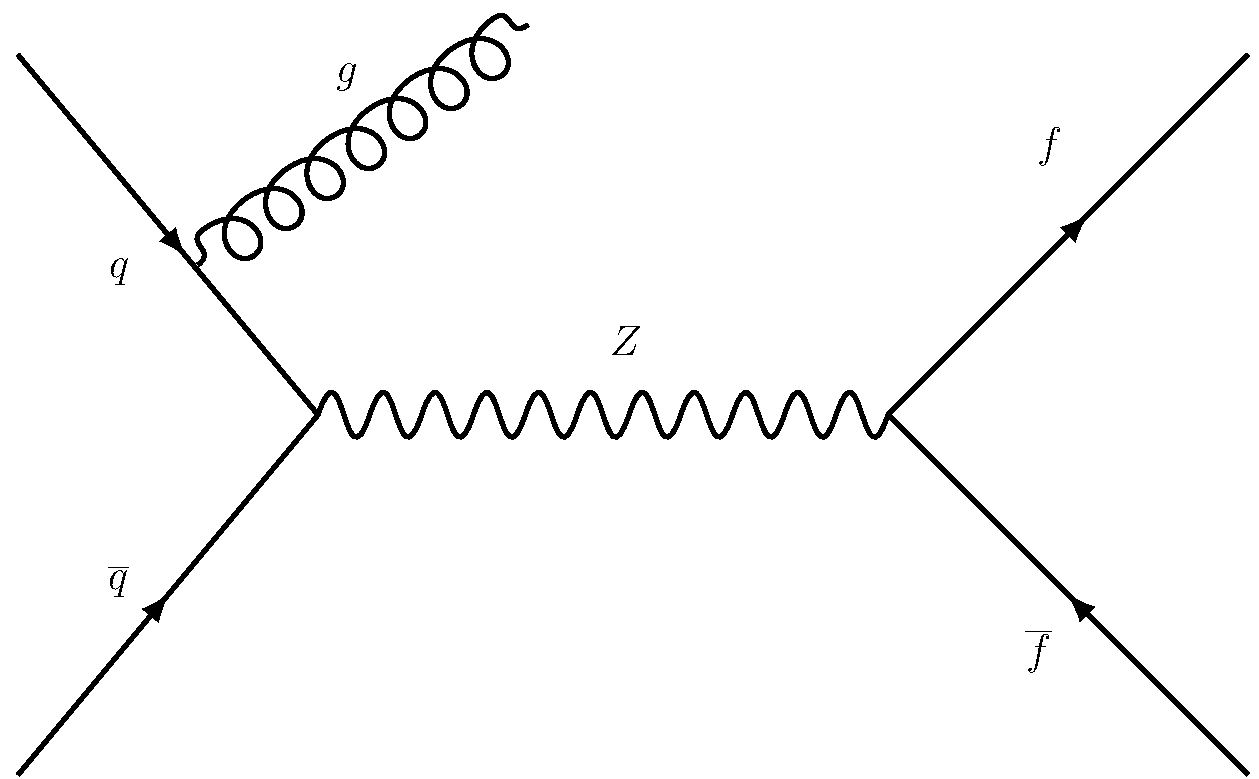
\includegraphics[width=0.50\textwidth]{figures/Fig16b}}}
	\caption{$qg$ Z boson production with FSR (a) and $q\bar{q}$ annihilation with gluon ISR (b).}
	\label{Fig16}
\end{figure}
\section{The Tau Lepton}\label{chap2sec1}
The tau is a spin-$\frac{1}{2}$ charged particle that belongs to the family of leptons. The first hints of the tau existence came from experiments conducted at the Stanford Linear Accelerator Center and Lawrence Berkeley National Laboratory \cite{PhysRevLett.35.1489}. They discovered 64 events of the form:
\begin{equation}
	e^+ + e^- \to e^\pm + \mu^\mp + \geq \text{2 undetected particles},
\end{equation}
for which there was no conventional explanation at the time. Later on, it was discovered that these events came from the production of a pair of new particles, two taus that subsequently decayed into one electron, a muon and four neutrinos. Events like,
\begin{equation}
e^+ + e^- \to \tau^+ \tau^- \to e^\pm + \mu^\mp + 4\nu,
\end{equation}	
were later explored to derive tau mass and spin, confirming the existence of a third generation of leptons. 
The tau has a mass of $1776.86 \pm 0.12$ MeV \cite{PhysRevD.98.030001}, which allows it to decay not only into the other lighter lepton generations (\textit{leptonic tau decays}), as shown on Fig.\ref{Fig1}  , but into hadrons. As we said on section \ref{chap2sec0} hadrons are particles made of quarks. All the decay channels of the tau containing hadrons in the final state are called \textit{hadronic tau decays}. Strictly speaking this is a semi-hadronic decay mode because of the presence of the neutrino. Nonetheless, from now on we will refer to these processes with the commonly used term \textit{hadronic tau decays}. An example of this decay mode is shown in Fig.\ref{Fig2}.
\begin{figure}[h]
	\centering
	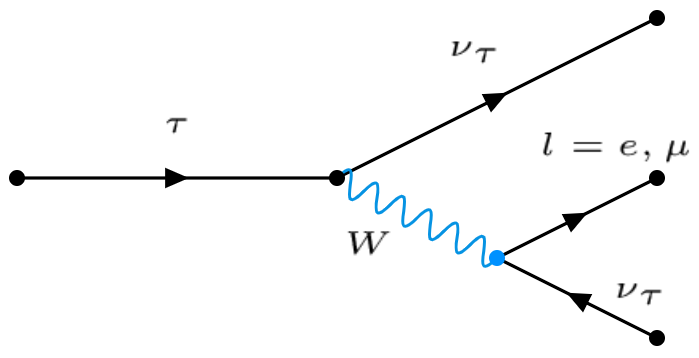
\includegraphics[width=0.6\textwidth]{figures/Fig1}
	\caption{Tau leptonic decay mode. Tau lepton is kinematically allowed to decay into muons or electrons, note that in this decay mode two neutrinos of different flavour are produced.}
	\label{Fig1}
\end{figure}
\begin{figure}[h]
	\centering
	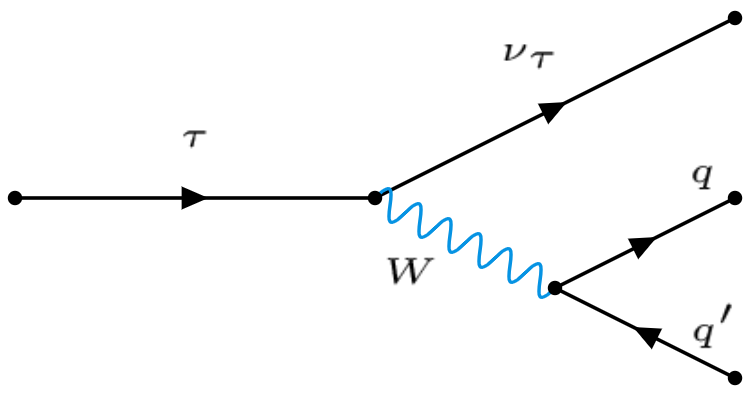
\includegraphics[width=0.6\textwidth]{figures/Fig2}
	\caption{Tau hadronic decay mode. The tau lepton is kinematically allowed only to decay into hadrons containing up, down and strange quarks. This results on final states containing multiple pions or kaons \cite{Davier_2006}.}
	\label{Fig2}
\end{figure}
The branching fraction for hadronic and leptonic tau decay modes is defined as
\begin{equation}
	\beta(\tau\to X\nu_\tau)=\frac{\Gamma(\tau\to X\nu_\tau)}{\Gamma_{\text{tot}}},
\end{equation}
where $X$ could be any number of leptons or hadrons and $\Gamma_{\text{tot}}$ is the total decay width for the tau. Naively, if we were to estimate it we could argue that the contribution from the hadronic decays triples the contribution for one of the leptonic modes. This is because in any hadronic decay, we would have to count 3 different diagrams, like the one in Fig.\ref{Fig2} because of the three colour possibilities for the quarks.

Thus, 
\begin{align}
\beta(\tau\to l\nu_l\nu_\tau)\approx 20\%& \hspace{1cm}l=e,\mu;
\\
\beta(\tau\to X\nu_\tau)\approx 60\%& \hspace{1cm} X=\text{hadrons+neutrinos}.
\end{align}
In fact, this naive estimation is not bad. Actual values for the leptonic branching ratios are \cite{PhysRevD.98.030001}:
\begin{align}
\beta(\tau\to e\nu_e\nu_\tau)&=17.82\pm 0.04\%
\label{eq6}
\\
\beta(\tau\to \mu\nu_\mu\nu_\tau)&=17.39\pm 0.04\%.
\end{align}
The reason for the difference in the estimation are the QCD corrections in the hadronic decays \cite{Pich:2013lsa}. The small difference between the leptonic branching fractions is due to the mass difference between the muon and the electron.

On the other hand, the hadronic decays of the tau are more varied and can contain many more particles in the final states. The vast majority of hadronic tau decays have charged or neutral pions in the final states, but more exotic decays including kaons also happen. Branching fractions for the most important tau hadronic decays are showed in Table \ref{Table1}.
\begin{table}[]
	\centering
\begin{tabular}{|c|c|}
	\hline
	Decay mode                     & Branching fraction \\ \hline
	$\pi^\pm \nu_\tau$             & 11.1 \%            \\ \hline
	$\pi^\pm \pi^0 \nu_\tau$       & 25.4\%             \\ \hline
	$\pi^\pm \geq 2\pi^0 \nu_\tau$ & 9.1\%               \\ \hline
	$3\pi^\pm \nu_\tau$            & 9.1\%               \\ \hline
	$3\pi^\pm \geq 1\pi^0 \nu_\tau$& 4.6\%               \\ \hline
	others						   & 5.5\%               \\ \hline
\end{tabular}
	\caption{Branching fractions for hadronic tau decay modes \cite{PhysRevD.98.030001}.}
	\label{Table1}
\end{table}
\section{Lepton Universality}\label{chap2sec2}
The SM predicts that all charged leptons $(e,\mu,\tau)$ interact via the electroweak force and explains that these interactions can be seen as the interchange of \textit{vector bosons}, the photon $(\gamma)$ and the W and Z bosons. Specifically, in the SM the form of the interaction does not depend on the lepton generation. This feature of the SM is called \textit{lepton universality} and is the fact that the couplings of the electrons, muons and taus to the electroweak bosons are identical. 

For instance, tau leptonic decay widths present a great opportunity to test lepton universality hypothesis. If we start considering muon decay, at low energies we can consider this process to be a point like interaction well described by Fermi theory \cite{FermiTheory}. In this case, if we approximate the electron and neutrinos as being massless particles, a dimensionally correct expression for the width is of the form
\begin{equation}
	\Gamma(\mu\to e+\nu_e +\nu_\mu)=KG_{F}^{2}m_{\mu}^{5},
\end{equation} 
where $G_F=1.1666\times 10^{-5} \text{ GeV}^{-2}$ is the Fermi coupling constant and $K$ is a constant that depends on the form of the interaction. If we assume that lepton universality holds, the respective widths for the tau leptonic decay modes, will have the form
\begin{align}
\Gamma(\tau\to e+\nu_e +\nu_\tau)&=KG_{F}^{2}m_{\tau}^{5},
\\
\Gamma(\tau\to \mu+\nu_\mu +\nu_\tau)&=\Gamma(\tau\to e+\nu_e +\nu_\tau),
\end{align}  
which explains why to a good approximation leptonic branching fractions for tau decay are equal. Moreover, we can obtain a relation between tau and muon lifetimes. We know that,
\begin{equation}
	\tau_l=\frac{1}{\Gamma_\text{Tot}}=\frac{\beta(l\to e\nu_e \nu_l)}{\Gamma(l\to e\nu_e \nu_l)},
	\label{eq11}
\end{equation}
also that $\beta(\mu\to e\nu_e \nu_\mu)=1$ and taking into account eq.(\ref{eq6}) we can take the ratio between eq.(\ref{eq11}) for $l=\tau ,\mu$ to obtain
\begin{equation}
\frac{\tau_\tau}{\tau_\mu}=\frac{\beta(\tau\to e\nu_e \nu_\tau)}{\beta(\mu\to e\nu_e \nu_\mu)}\left(\frac{m_\mu}{m_\tau}\right)^5=(1.328\pm 0.004)\times 10^{-7}.
\end{equation}
This is consistent with the experimental lifetimes ratio of $(1.3227\pm 0.0005)\times10^{-7}$ \cite{Martin:1992rg}. This agreement on lifetimes that differ by seven orders of magnitude is a good proof that lepton universality holds on W decays at the tau mass scale.

Very precise tests of LU have been done by $e^-e^+$ colliders (LEP1, SLC and LEP2). Measurements of the ratios between the leptonic decay widths of the Z boson have been performed and are consistent with the SM \cite{ALEPH:2005ab}:
\begin{align}
	\frac{\Gamma(Z\to\mu^+\mu^-)}{\Gamma(Z\to e^+e^-)}=1.0009\pm 0.0028,
	\\
	\frac{\Gamma(Z\to\tau^+\tau^-)}{\Gamma(Z\to e^+e^-)}=1.0019\pm 0.0032.
\end{align}
LU has also been tested in W boson decays. A combination of measurements made by different experiments of the branching fractions between the first two families of leptons are consistent with SM predictions \cite{Pich:2013lsa}:
\begin{equation}
\frac{\beta(W^-\to e^-\bar{\nu_e})}{\beta(W-\to \mu^-\bar{\nu_\mu})}=1.004\pm 0.008.
\end{equation}
However, measurements including the third lepton family, apart from being less precise due to the more challenging reconstruction of the $\tau$ lepton final states are in tension with SM \cite{Schael:2013ita}:
\begin{align}
\frac{\Gamma(W^-\to\tau^-\bar{\nu_\tau})}{\Gamma(W^-\to e^-\bar{\nu_e})}=1.063\pm 0.027,
\\
\frac{\Gamma(W^-\to\tau^-\bar{\nu_\tau})}{\Gamma(W^-\to \mu^-\bar{\nu_\mu})}=1.070\pm 0.026.
\end{align}
These results show that LU between the two first lepton family holds with a precision of 0.3\% and 0.8\% in Z and W decays respectively. Constraints between the third and the other two generations of leptons are of similar precision on Z boson decays (0.3\%), but ten times worse for W boson decays (3\%) and somewhat in tension with SM prediction. %%An example of this is a measurement exhibiting a tension of 2.6 $\sigma$ from the SM expectation \cite{Schael:2013ita}:
%%\begin{equation}
	%%\frac{2\Gamma(W^-\to\tau^-\bar{\nu_\tau})}{\Gamma(W^-\to e^-\bar{\nu_e})+\Gamma(W^-\to %%\mu^-\bar{\nu_\mu})}=1.066\pm 0.025.
%%\end{equation}  


Furthermore, measurements from LHCb, BaBar and Belle experiments have shown consistent deviations from the SM predictions \cite{Ciezarek_2017}. These experiments have independently measured a deviation on $\bar{B}$ meson semi-leptonic branching ratios, specifically:
\begin{align}
	R_D&=\frac{\beta(\bar{B}\to D\tau^-\bar{\nu}_\tau)}{\beta(\bar{B}\to De^-\bar{\nu}_e)}
	\\
	R_{D^\star}&=\frac{\beta(\bar{B}\to D^\star\tau^-\bar{\nu}_\tau)}{\beta(\bar{B}\to D^\star e^-\bar{\nu}_e)}.
\end{align}
The combined results for the different experiments are shown in Fig.\ref{Fig3}. These measurements represent a 3.08 $\sigma$
 deviation from the SM predictions, but even though they represent a hint of new physics, higher statistical precision will be needed to confirm this results. Future analysis from experiments like LHCb and Belle II with larger available datasets will be very important to untangle this situation.
 \begin{figure}[h]
 	\centering
 	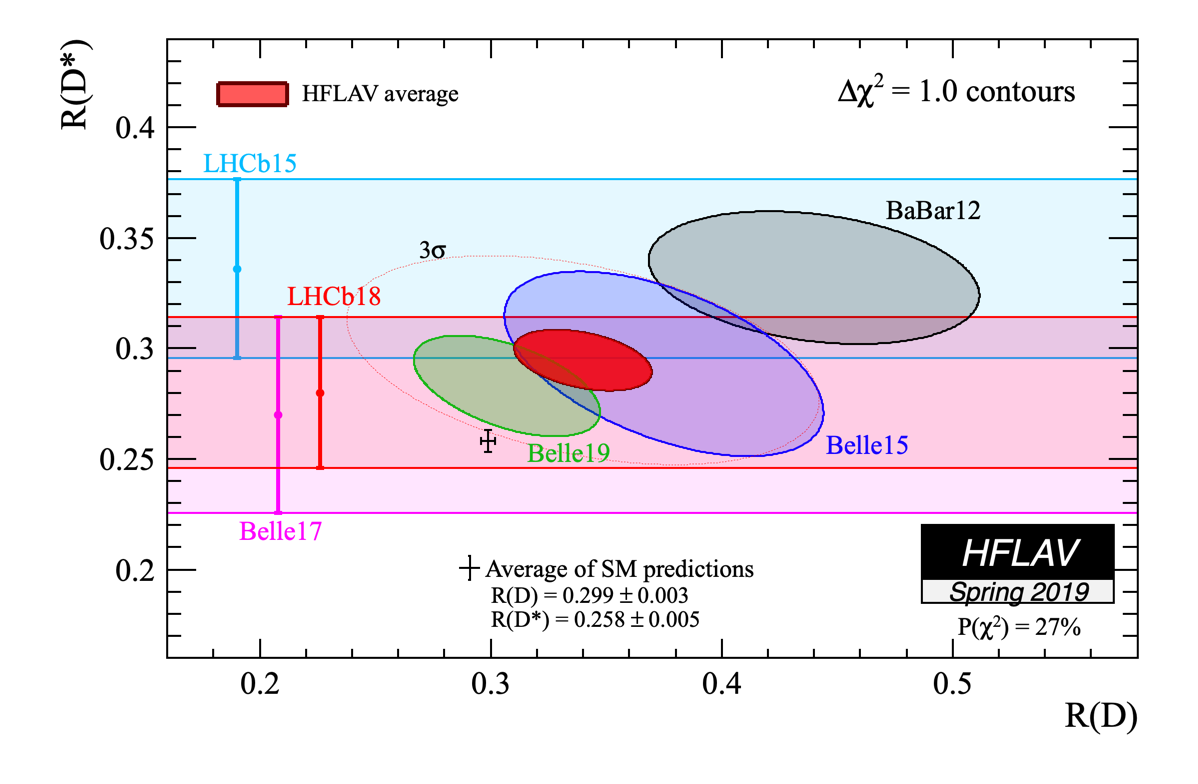
\includegraphics[width=0.7\textwidth]{figures/Fig3}
 	\caption{Combined results from BABAR, Belle and LHCb with 1-$\sigma$ contour. The average calculated by the Heavy Flavour Averaging Group \cite{HFAG}  is compared with the SM predictions.}
 	\label{Fig3}
 \end{figure}
    \chapter{Tau Reconstruction and Identification on ATLAS}\label{ATLAS}
In this chapter, a review of the ATLAS detector at the Large Hadron Collider and a description of the reconstruction and identification of hadronic Tau decays on ATLAS are presented.
\section{The LHC and the ATLAS experiment}
The Large Hadron Collider (LHC) is the largest particle accelerator currently operated by the European Organization for Nuclear Research (CERN). The LHC uses a 27 km tunnel where 2090, 15 m long, dipolar superconducting magnets bend the trajectories of two proton beams going in opposite directions. Each of the magnets is capable of producing a 8,33 T magnetic field and thus bending protons with an energy up to 7 TeV. The magnets are cooled down to 1.9 K in order to reach the superconducting state and the vacuum inside the tubes is of the order of $10^{-9}$ mbar. During Run II, proton beams were accelerated to an energy of 6.5 TeV and they are collided in 4 interaction points where the detector experiments are located.

One of these experiments is the ATLAS (A Toroidal LHC ApparatuS) detector. It is a multi-purpose particle detector, capable of discovering new physics but also perform high precision SM measurements, a complete description of the ATLAS design can be found at \cite{ATLAS:1999uwa}. ATLAS is a cylindrical detector composed by sub-detectors arranged in shells. The most inner layers are surrounded by a superconducting solenoid that generates a 2 T solenoidal magnetic field. ATLAS uses a right-handed coordinate system with its origin at the interaction point (IP) in the centre of the detector, the z-axis points along the beam pipe. The x-axis points towards the centre of the LHC ring and the y-axis along the azimuth direction. The angle $\phi$ is defined in the $x-y$ plane and pseudorapidity is defined in terms of the polar angle $\theta$ as $\eta=-\log \tan(\theta/2)$. The angular distance is measured in units of $\Delta R\equiv \sqrt{(\Delta\phi)^2+(\Delta\eta)^2}$.

The most inner detector is in charge of vertex reconstruction and it consist of a silicon pixel, silicon microstrip and transition radiation tracking detectors. The system has a coverage of $|\eta|<2.5$. The tracker system is followed by a lead/liquid-argon electromagnetic calorimeter (EC) and a steel/scintillator-tile hadron calorimeter (HC) that provide energy measurements with high granularity for electromagnetic showers and hadrons. The end-cap and forward EC and HC use LAr technology detectors and extend up to a $|\eta=4.9|$ region. The outermost detection system is a muon spectrometer that takes advantage of the bending power of a system of three air-core toroidal superconducting magnets.
  
\section{Tau Reconstruction and Identification on the ATLAS detector}
Leptonically decaying taus ($\tau_\text{lep}$), may have a higher impact parameter and tend to have a softer $p_T$ spectrum compared with prompt W or Z boson decays to muons or electrons. This variables are not sufficient in principle to differentiate between $\taul$ and prompt muons or electrons. In the case of hadronically decaying taus ($\tau_\text{had}$), as we will see, there are a lot more variables we could use to tag the presence of a $\tauh$.

As we saw in section \ref{chap2sec1}, $\tauh$ decays can be classified in 1-prong or 3-prong, depending on the number of charged particles in the decay. A detailed review of the reconstruction procedure is discussed on \cite{Aad:2014rga}. $\tauh$ candidates are seeded by jets using the anti-$k_t$ algorithm \cite{Cacciari:2008gp}, with a distance parameter of 0.4. Jets are required to have $p_T>10$ GeV and $|\eta|<2.5$. Candidates between the barrel and forward calorimeter ($1.37<|\eta|<1.52$) are excluded due to poor instrumentation in this region.

The axis of the seed jet is defined by the energy-weighted barycentre of all clusters of calorimeter cells, called \textit{TopoClusters} \cite{Aad:2016upy}. The $\tauh$ vertex is defined as the vertex with the highest $p_T$-weighted fraction of all tracks with $p_T>0.5$ GeV within a cone of $R=0.2$ around the seed jet axis. Tracks within a cone of $R=0.4$ are classified with a set of boosted decision trees (BDTs) into core and isolation tracks, the number of core tracks defines the number of prongs. Candidates with neither one or three tracks are rejected. Additionally, the sum of the charge of the tracks is required to be $\pm 1$.     

The tau reconstruction algorithm does not provide discrimination against jets that could mimic the signal of a $\tauh$ decay in the detector. Therefore, algorithms that perform this task have been developed. Previously, a BDT was used to discriminate jets against $\tauh$. Recently, a recurrent neural network (RNN) classifier that provides improved performance than the BDTs is in use \cite{Deutsch:2680523}.

The RNN makes use of a set of variables like: $\tauh$ track features, information about energy deposits on the calorimeters clusters and high level features like the mass of the $\tauh$ candidate tracks. This variables are used to exploit the differences in the shapes of the showers between $\tauh$ and jets. In general, $\tauh$ showers tend to be more collimated and to have fewer tracks than jets. A representation of this is shown in Fig.\ref{Fig4}. 

\begin{figure}[h]
	\centering
	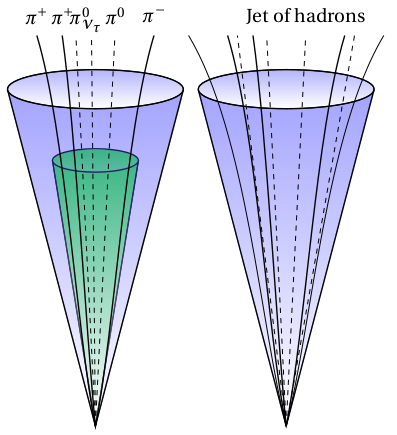
\includegraphics[width=0.7\textwidth]{figures/Fig4}
	\caption{Graphic representation that shows the main differences between a 3-prong $\tauh$ and a jet originated from quark or gluon radiation (QCD jets). Charged hadrons are shown as thick lines and dashed lines represent neutral particles. The green cone is drawn to depict how $\tauh$ product decays are more collimated.}
	\label{Fig4}
\end{figure}
Separated algorithms are trained for 1-prong and 3-prongs. The final RNN score assigned to each event corresponds to the fraction of rejected true $\tauh$, independent of $p_T$ and number of interaction per bunch crossing (pileup). Four working points with increasing background rejection are defined to be used in physics analysis. The working points and background rejection factors are shown in Table \ref{Table2}. A plot comparing the true $\tauh$ selection efficiency versus the background rejection power for the RNN and BDT algorithm is shown in Fig. , the performance of the RNN is better than the BDT classifier. Finally, the distribution for the RNN score for true and fake $\tauh$ is shown in Fig. , for both 1-prong and 3-prong decays.
\begin{table}[]
	\begin{tabular}{|l|l|l|l|l|l|l|}
		\hline
		Working point & \multicolumn{2}{l|}{Singal efficiency (\%)} & \multicolumn{2}{l|}{BG rejection BDT} & \multicolumn{2}{l|}{BG rejection RNN} \\ \hline
		& 1-prong              & 3-prong              & 1-prong               & 3-prong               & 1-prong               & 3-prong               \\ \hline
		Tight         & 60                   & 45                   & 40                    & 400                   & 70                    & 700                   \\ \hline
		Medium        & 75                   & 60                   & 20                    & 150                   & 35                    & 240                   \\ \hline
		Loose         & 85                   & 75                   & 12                    & 61                    & 21                    & 90                    \\ \hline
		Very loose    & 95                   & 95                   & 5.3                   & 11.2                  & 9.9                   & 16                    \\ \hline
	\end{tabular}
	\caption{Working points with their corresponding true $\tauh$ selection efficiency and the background rejection factors. The scores are shown for both RNN and BDT algorithms.}
	\label{Table2}
\end{table}
\begin{figure}[h]
	\centering
	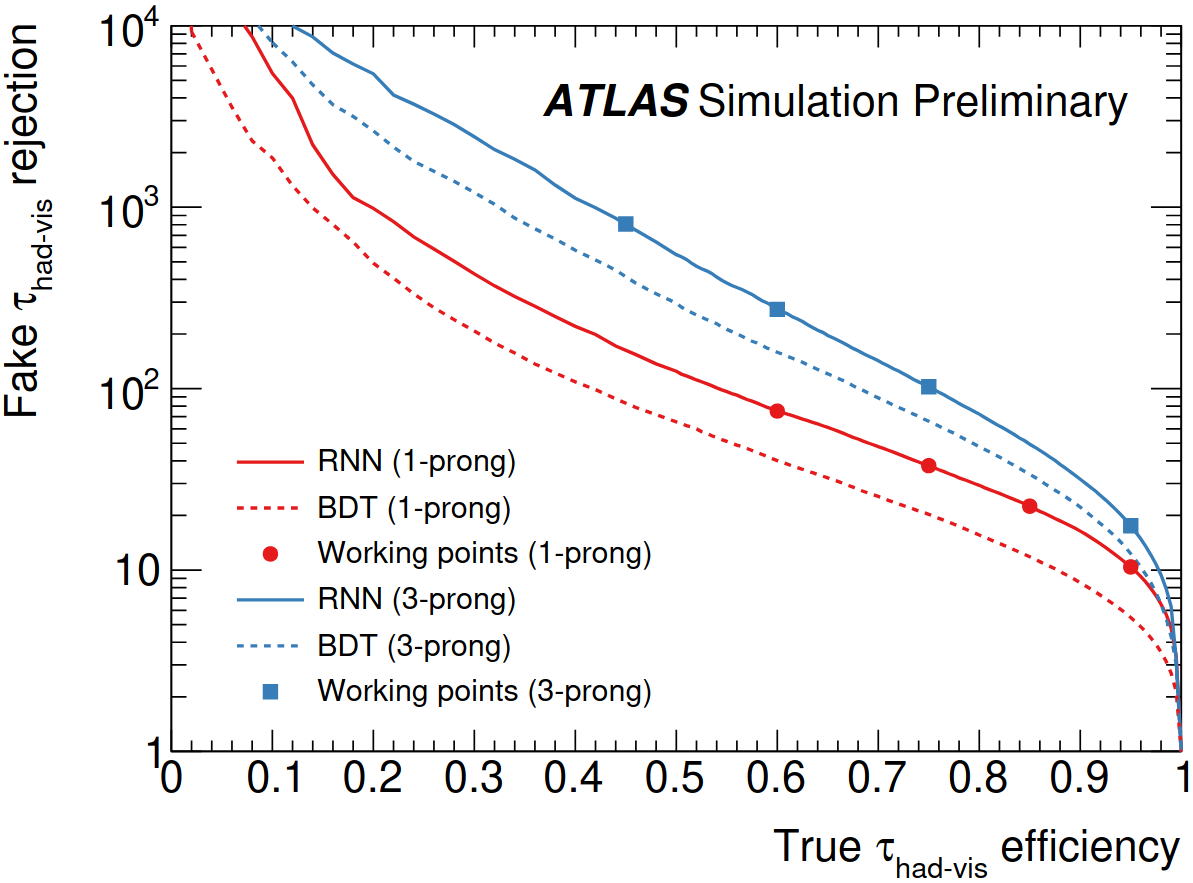
\includegraphics[width=0.7\textwidth]{figures/Fig5}
	\caption{Comparisson between the performance of BDT and RNN algorithms. Working points are shown as points. Notice there is a trade off between true $\tauh$ efficiency and background rejection power. Taken from \cite{Deutsch:2680523}}
	\label{Fig5}
\end{figure}
\begin{figure}[h]
	\centering
	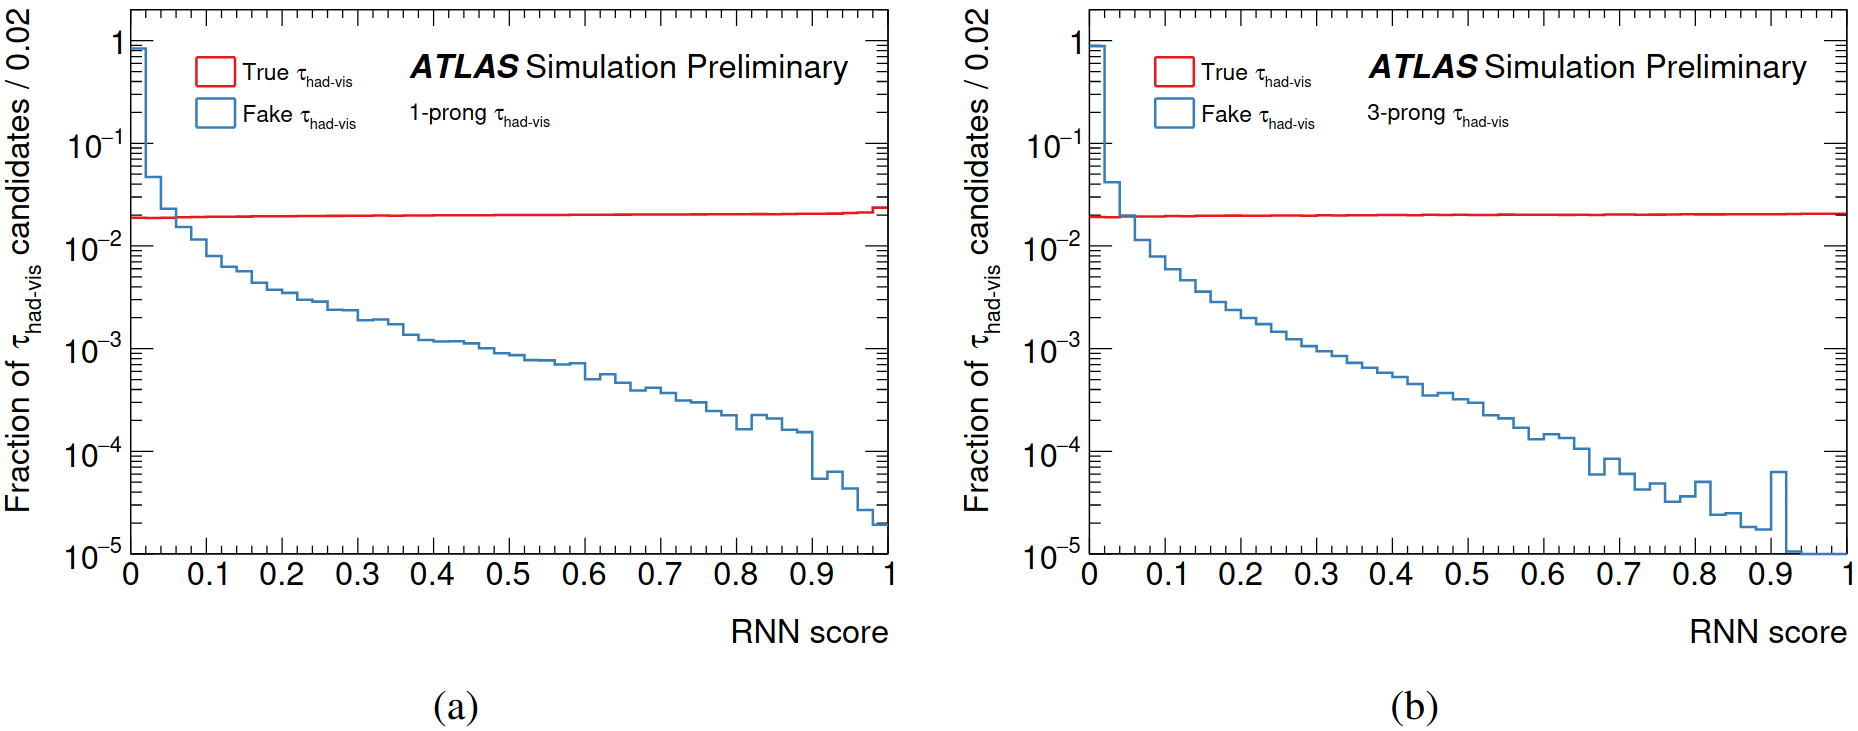
\includegraphics[width=1\textwidth]{figures/Fig6}
	\caption{Distribution of the RNN scores for true and fake $\tauh$ candidates for 1-prong (a) and 3-prong (b) cases. Taken from \cite{Deutsch:2680523}.}
	\label{Fig6}
\end{figure}
    \chapter{$Z\to\tauh\taul$ tag and probe study}\label{chap1}
This chapter describes the analysis methodology of using $Z\to\tau\tau$ events to measure Monte Carlo correction factors for tau identification algorithms in the high-$p_T$ region.

As we saw in the previous section different working points are defined for RNN score relative to the efficiency of selecting true $\tauh$ candidates. When the efficiency of the working points is measured in data and simulation, a correction factor is derived and then applied to the simulation in order for the signal efficiency to agree between data and simulation \cite{ATLAS:2017mpa}. Because of the top quark mass, $t\bar{t}$ events are used as a source of high momentum taus for measuring correction factors on the high-$p_T$ bins. But as we already saw in section \ref{chap2sec2}, Lepton universality may not hold in W decays. For that reason our study is aimed to use $Z\to\tau\tau$ events for deriving and cross checking simulation correction factors in the high-$p_T$ region.   

\section{Signal events}\label{chap4sec1}
The type of $Z\to\tau\tau$ events we consider as signal for this study are when one the taus decays hadronically and the other leptonically, either into an electron or a muon ($Z\to\tau\tau\to\tau_h +l=\mu,e$). Thus, our final states will include a $\tauh$ candidate and a lepton $l=e,\mu$. The presence of this lepton will be used as our tag. 
Generally, in $Z\to\tau\tau$ events, the taus are produced back to back and their $\pt$ spectrum does not go very high. One way to select events where the taus are boosted in the transverse plane is to look for events where the opening angle in the transverse plane between the taus ($\Delta\phi(\tauh,\taul)$) is more acute. For these events, the missing transverse momentum ($\ptmiss$) is assumed to come from the neutrinos produced in the decays of the tau leptons. Due to the fact that two neutrinos are produced in the leptonic decay mode we expect our events to have a larger $\ptmiss$ component along the $\taul$ direction.

We classify our events in two types of topologies. First, events where the $\ptmiss$ is inside the opening angle between the visible objects, in this kind of events we assume the missing energy is due to a pair of neutrinos flying in the same direction as the visible objects. This is shown in Fig.\ref{Fig7a}. In this case, we solve the following equation to obtain the momentum of the neutrinos:
\begin{equation}
	\vec{p}_{T_{\nu_l}}+\vec{p}_{\nu_h}=\vec{\ptmiss},
\end{equation}
given the following set of constraints (\textit{collinear approximation}):
\begin{align}
	\phi(\nu_l)&=\phi(l),
	\\
	\phi(\nu_h)&=\phi(\tauh),
	\\
	\eta(\nu_l)&=\eta(l),
	\\
	\eta(\nu_h)&=\eta(\tauh).
\end{align}
The second case is when the $\ptmiss$ is outside the angle formed by the visible objects, as is shown in Fig.\ref{Fig7b}. In this case the assumption is that only one neutrino is responsible for the majority of the $\ptmiss$, a neutrino flying in the direction of the visible object that is closest to the $\ptmiss$. We use the following equations to obtain the neutrino momentum:
\begin{align}
p_{T_{\nu}}&=\ptmiss \cos(\Delta\phi(\tau_{\text{closer}},\ptmiss)),
\\
\phi(\nu)&=\phi(\tau_{\text{closer}}),
\\
\eta(\nu)&=\eta(\tau_{\text{closer}}),
\end{align} 
\begin{figure}[ht]
	\centering
	\subfloat[]{\label{Fig7a}{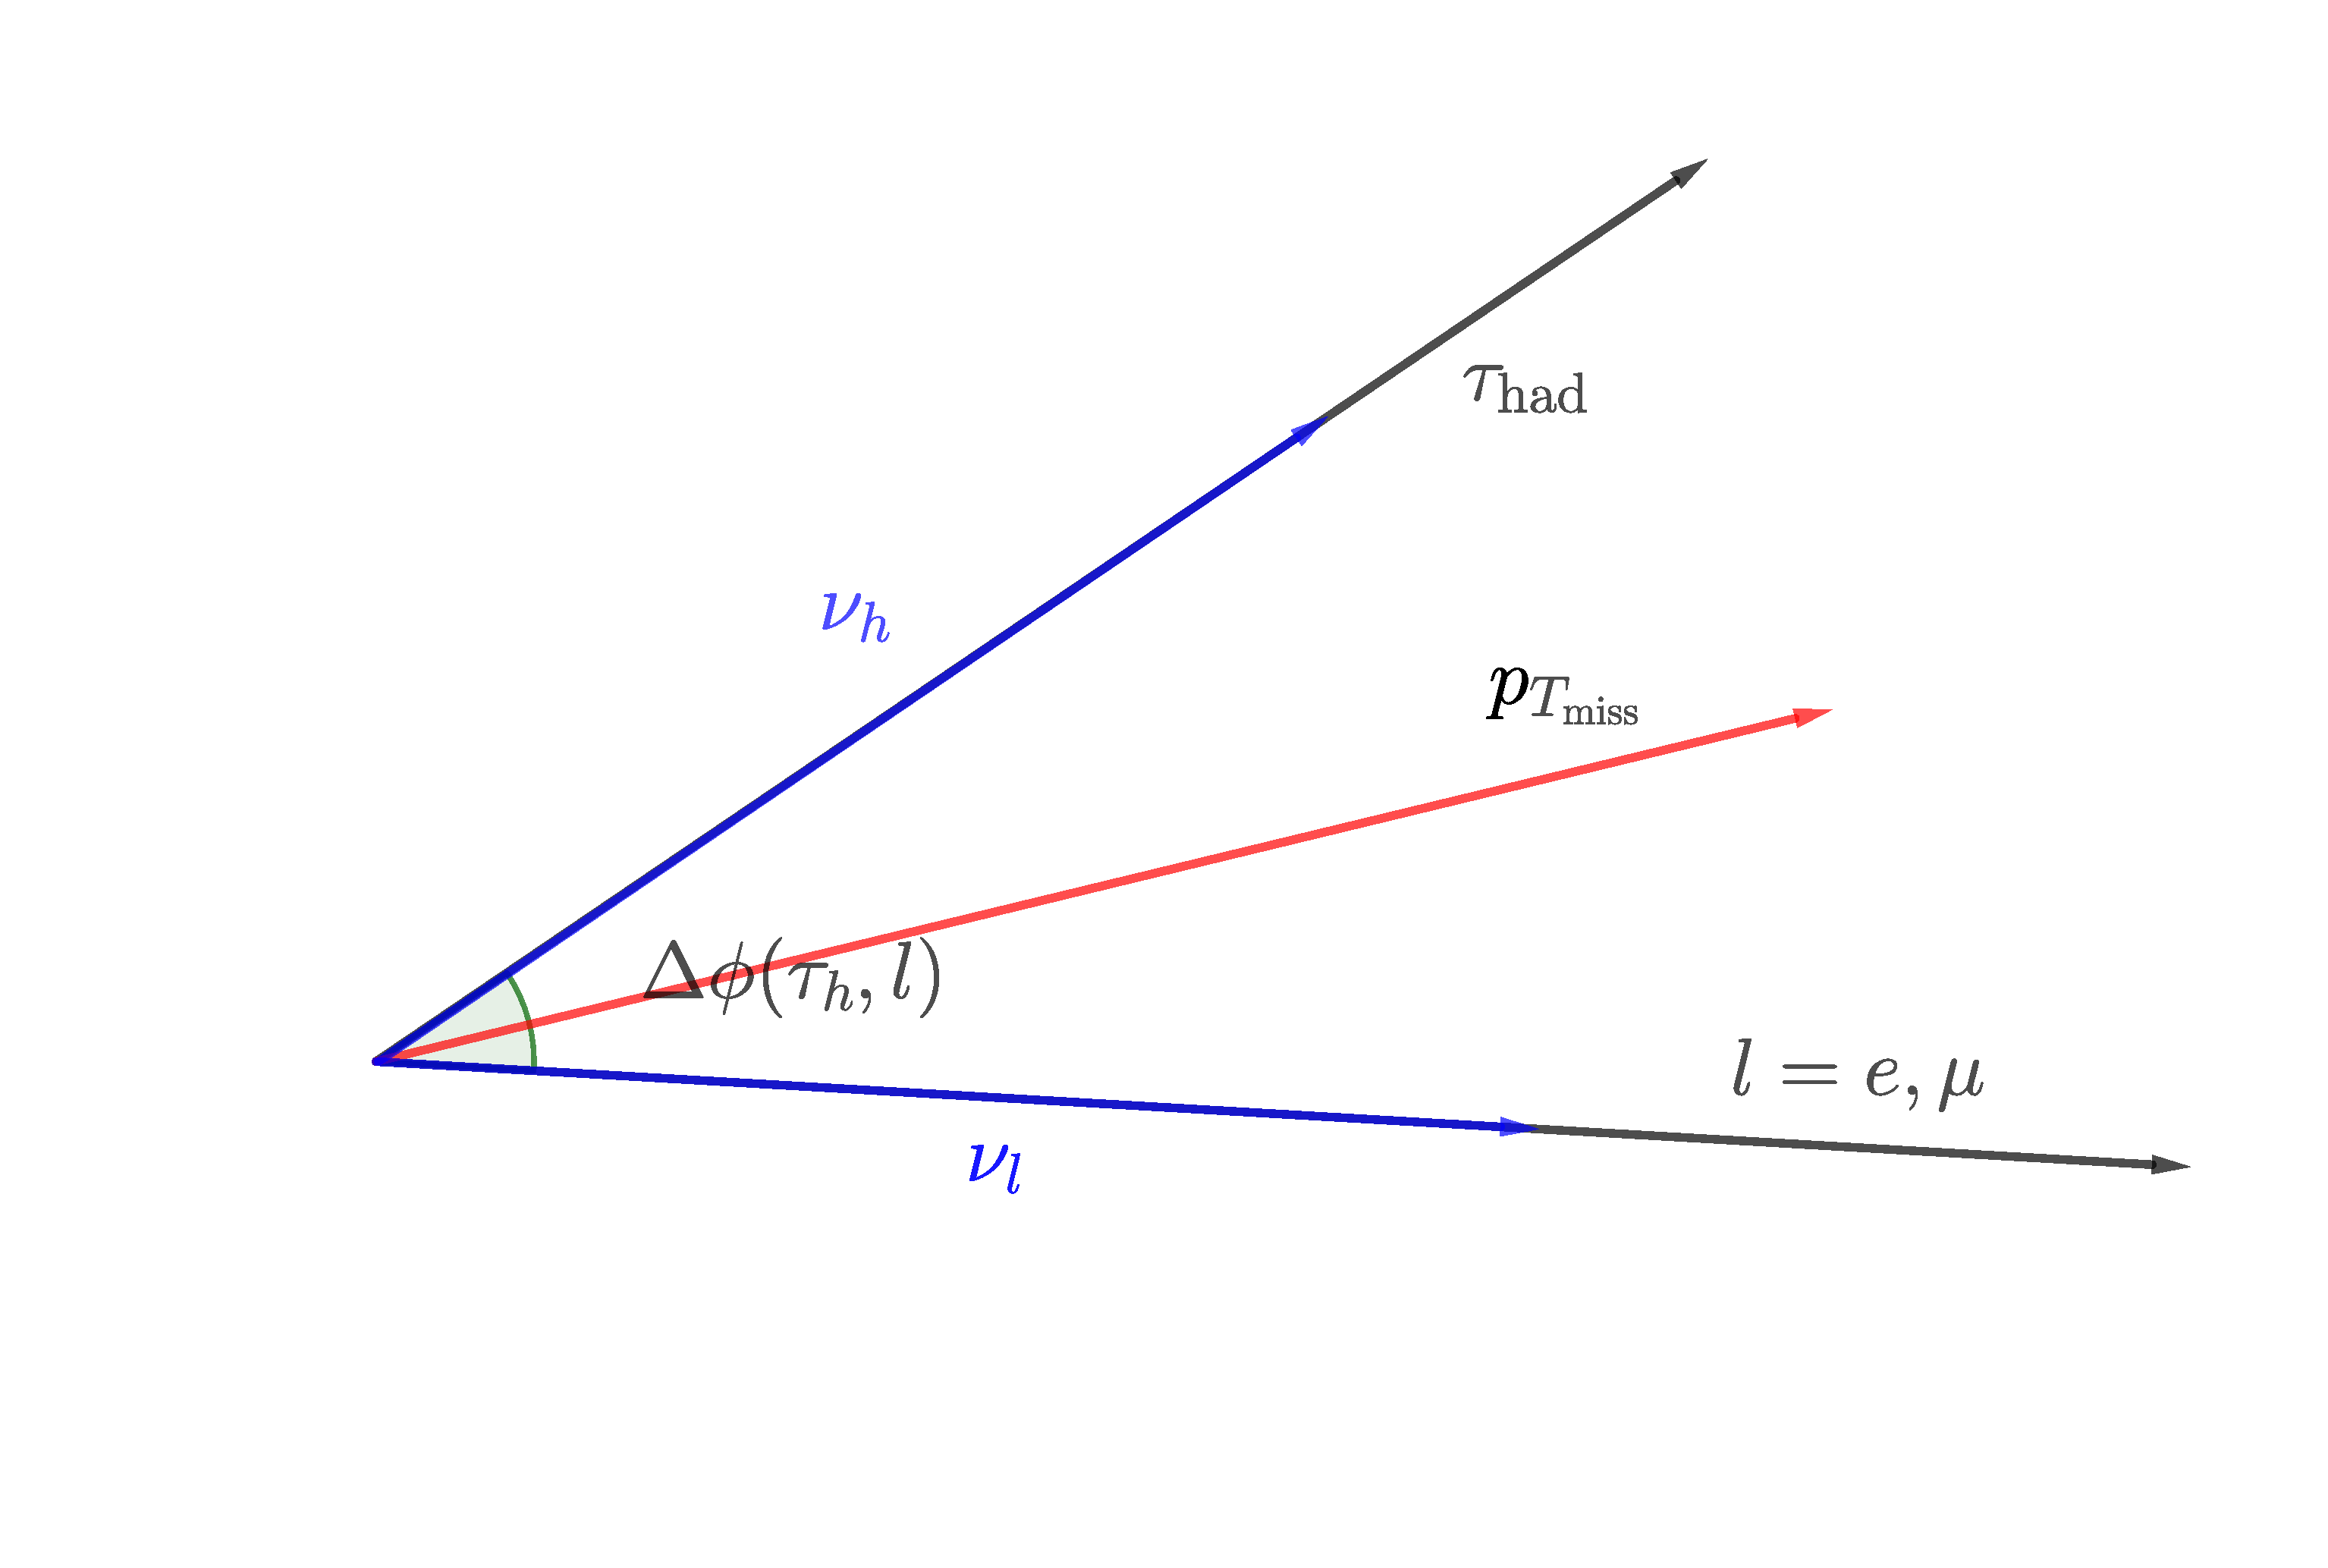
\includegraphics[width=0.49\textwidth]{figures/Fig7a}}}\hfill
	\subfloat[]{\label{Fig7b}{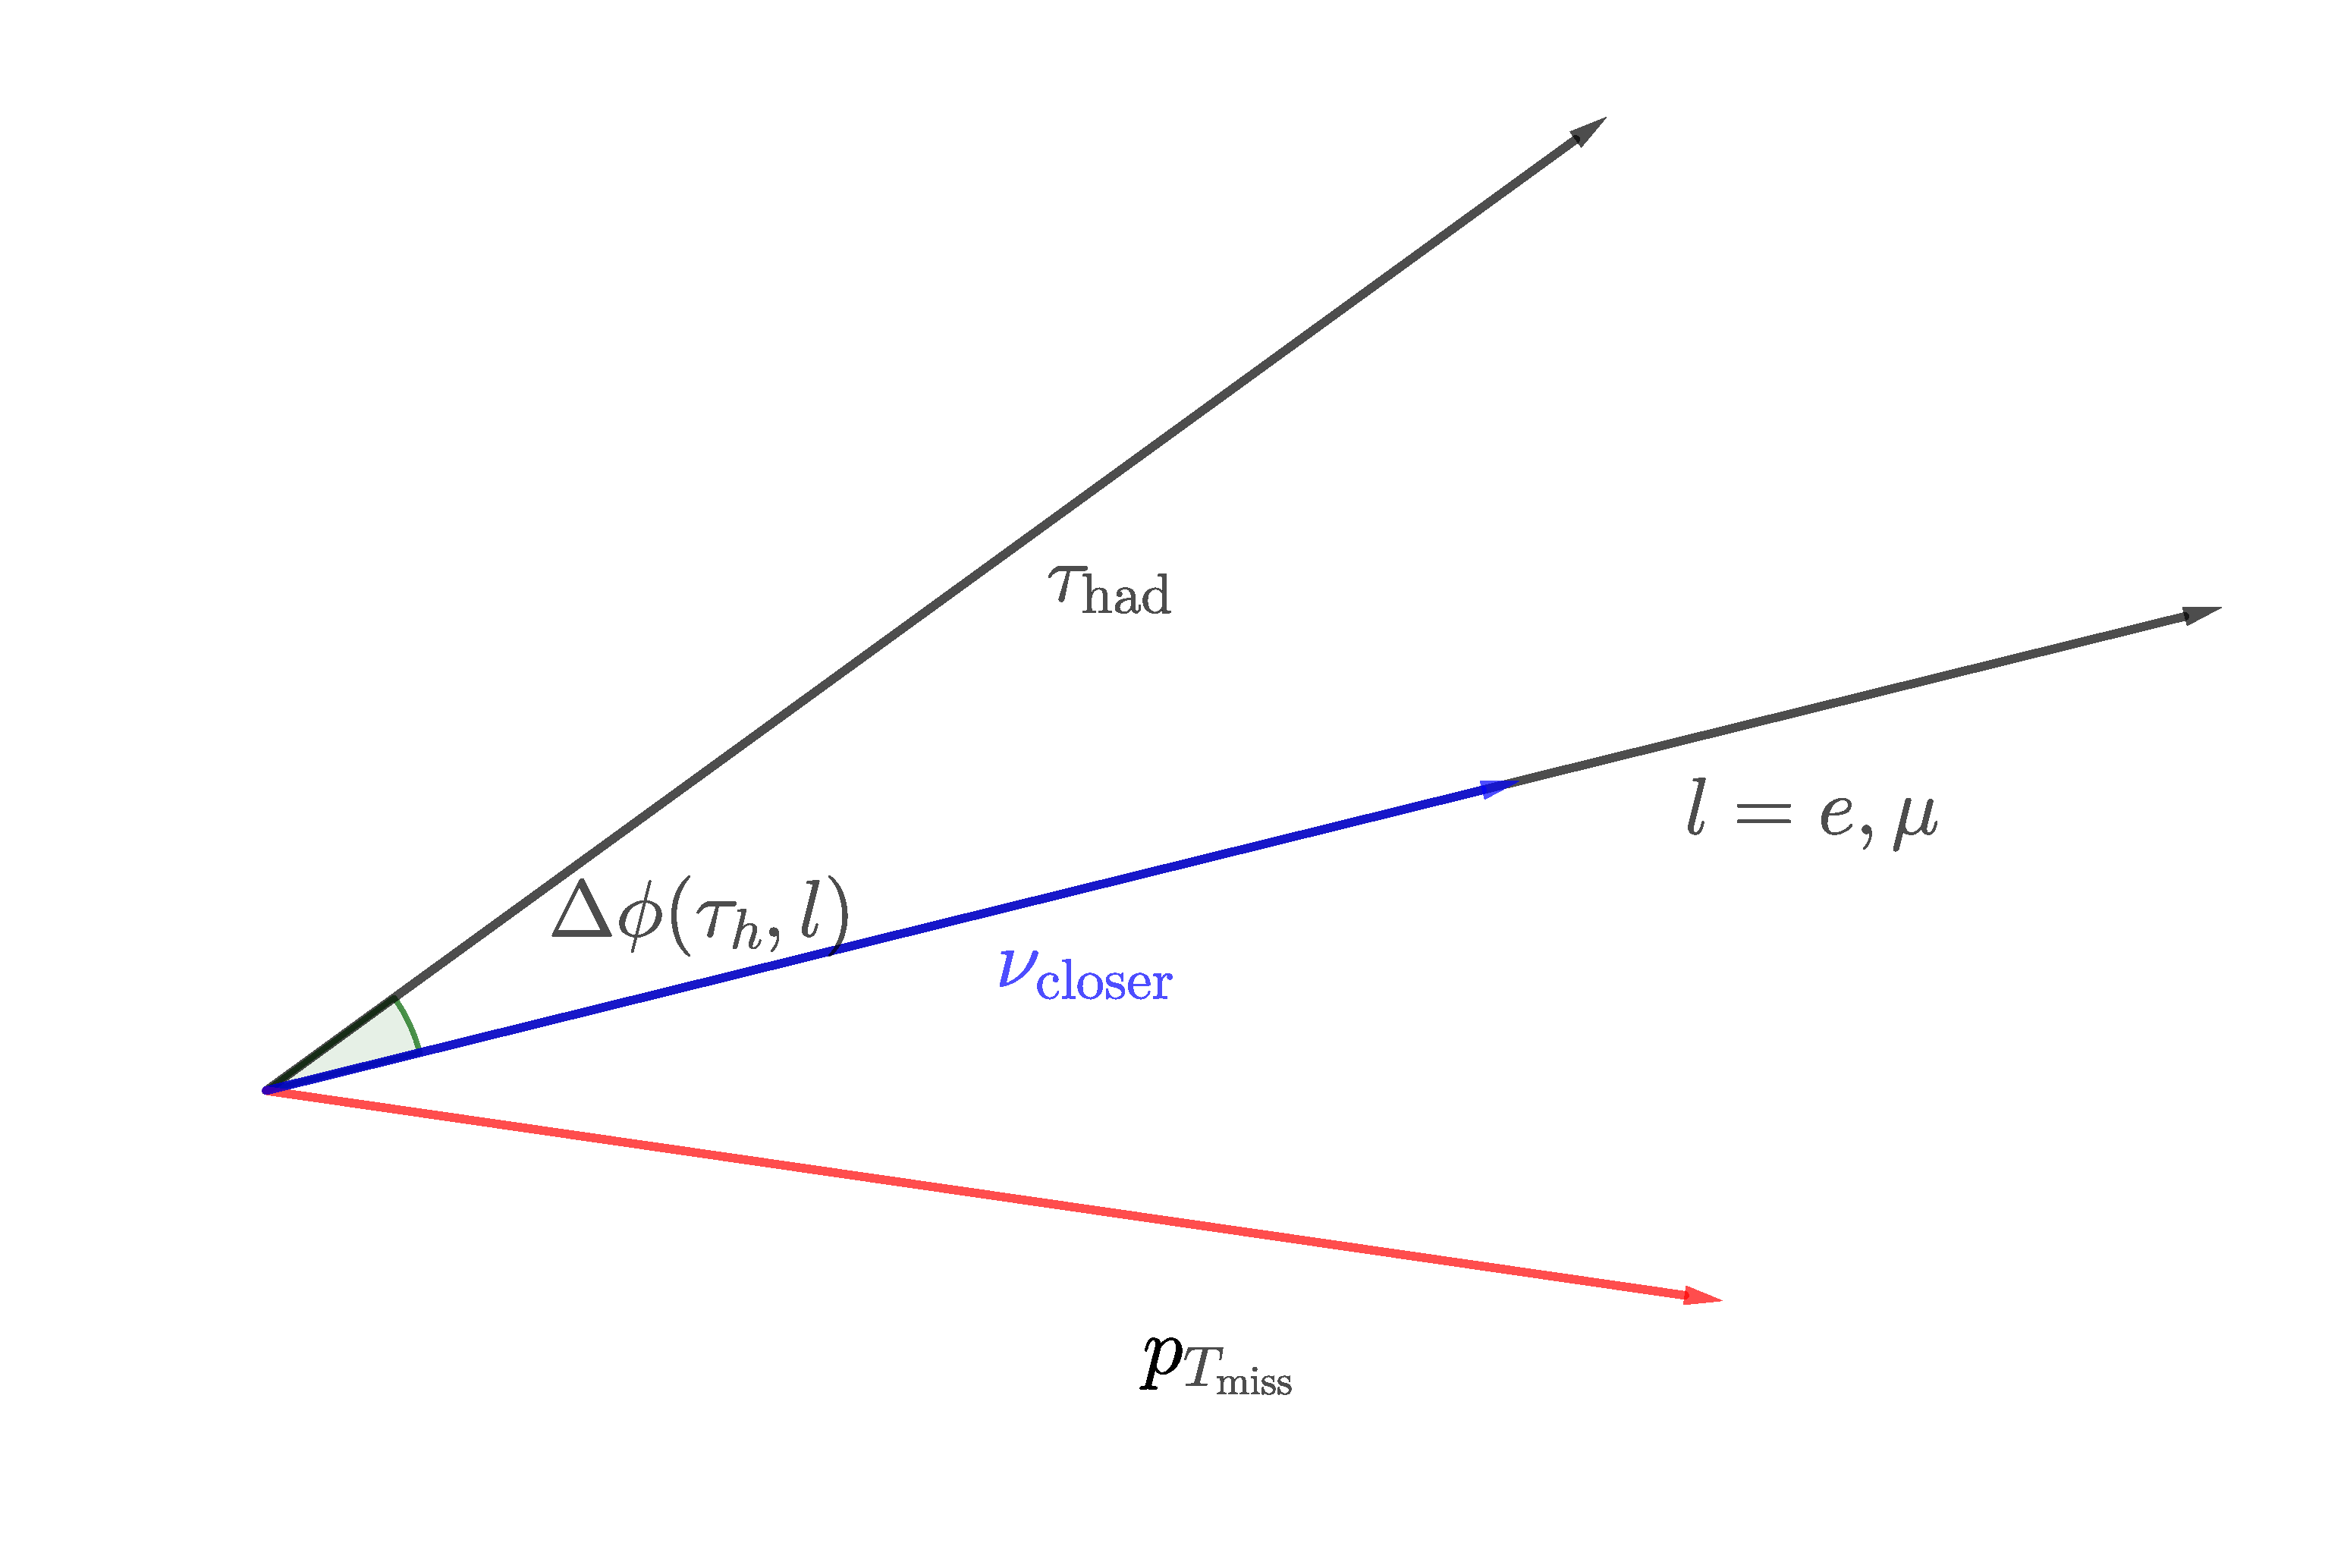
\includegraphics[width=0.49\textwidth]{figures/Fig7b}}}
	\caption{The two different types of topologies that define signal events. On the right, when the missing energy is between the visible objects two neutrinos are assumed to be responsible for all the missing energy. On the left, only one neutrino is assumed to be flying on the direction of the visible object closest to the missing energy.}
	\label{Fig7}
\end{figure}
where $\tau_{closer}$ stands for the visible object closest to the direction of the missing energy.

We define a variable called $\Omega$ in order to classify our events in the different topologies already described. First we define:
\begin{equation}
	\omega=\frac{\Delta\phi(\tau_{\text{close}},\ptmiss)}{\Delta\phi(\tauh,\taul)},
\end{equation}
then,
\begin{itemize}
	\item when $\ptmiss$ is inside the opening angle between the visible objects but closer to $\tauh$:
	\begin{equation}
		\Omega=\omega,
	\end{equation}
	\item when $\ptmiss$ is still inside, but closer to $\taul$:
	\begin{equation}
		\Omega=1-\omega.
	\end{equation}
	\item If $\ptmiss$ is outside and closer to $\tauh$:
	\begin{equation}
		\Omega=-\omega,
	\end{equation}
	\item and finally, if $\ptmiss$ is outside and closer to $\taul$:
	\begin{equation}
		\Omega=\omega+1.
	\end{equation}
\end{itemize}
Thus, $\Omega$ is a continuous variable that give us information on the topology of the event. When $\ptmiss$ is inside the visible system it has values in the interval [0,1]. Exactly 0 when $\ptmiss$ is in the $\tauh$ direction and 1 when is on the $\taul$ direction. $\Omega$ has negative values when $\ptmiss$ is outside and closer to the $\tauh$ candidate and has positive and values greater than 1 when is outside and closer to the $\taul$. A diagram describing the $\Omega$ values is shown in Fig.\ref{Fig8}.
\begin{figure}[h]
	\centering
	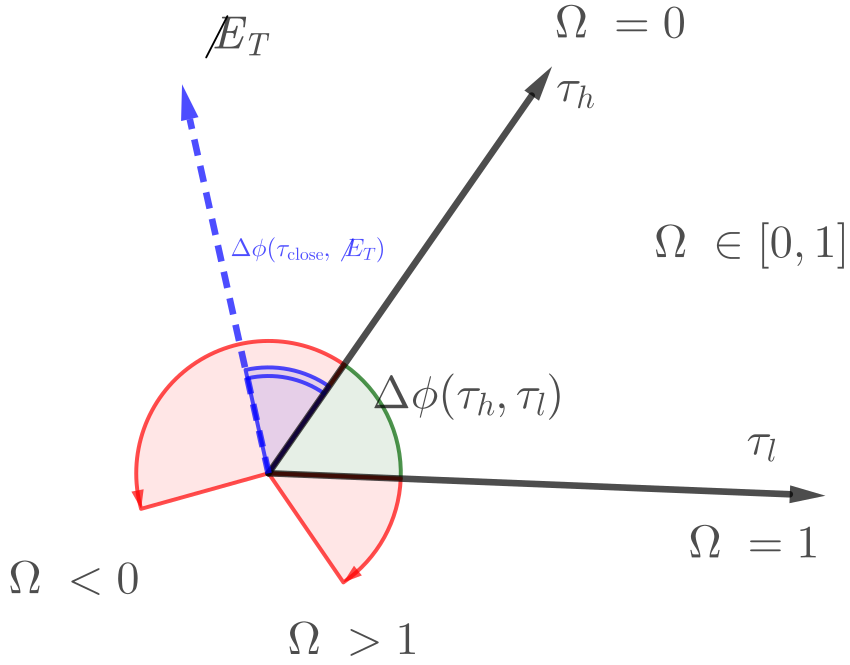
\includegraphics[width=0.5\textwidth]{figures/Fig8}
	\caption{Graphical representation of the different values of $\Omega$ depending on the region where the $\ptmiss$ is located in the event.}
	\label{Fig8}
\end{figure}
As we will see later the event classification into this two different type of topologies will allow us to reconstruct and exploit kinematical variables as the invariant mass of the di-tau system, the Z boson transverse momentum ($Z_{p_T}$) and the angular distribution of the objects in the event.
\section{Monte Carlo and Data Samples}
The data used for this study has been recorded during the Run-II of the LHC. It corresponds to the 2015-2018 data taking period, the total integrated luminosity corresponds to 139.2 $\text{fb}^{-1}$ of proton-proton collisions at a centre-of-mass energy of $\sqrt{s}=13$ TeV.

Monte Carlo (MC) samples are used for signal and background simulation. For $Z\to\tau\tau$ events two MC samples are used, Powheg+Pythia8 and Sherpa. For the rest of the samples Powheg+Pythia8 is used. Table \ref{Table3} shows the MC generators used for each process.

\begin{table}[]
	\centering
	\begin{tabular}{cc}
		\hline
		\multicolumn{1}{|c|}{Process}  & \multicolumn{1}{c|}{Event Generator} \\ \hline
		$Z\to\tau\tau$                 & Powheg+Pythia8 and Sherpa            \\
		$Z\to ee$                      & Powheg+Pythia8                       \\
		$Z\to\mu\mu$                   & Powheg+Pythia8                       \\
		$W\to l\nu_l$				   & Powheg+Pythia8                       \\
		$t\bar{t}$                     & Powheg+Pythia8                       \\
		Single $t$                     & Powheg+Pythia8                       \\
		Diboson                        & Powheg+Pythia8                       \\ \hline
	\end{tabular}
	\caption{List of MC event generators used.}
	\label{Table3}
\end{table}
\section{Event Selection}\label{chap4sec3}
In order to select $Z\to\tauh\taul$ events, our basic selection includes events with exactly one $\tauh$ candidate and one lepton, a muon or an electron. The $\tauh$ and lepton pair need to have opposite charge. As we said, the presence of the lepton will be used as our tag, thus, a lepton trigger is required to be fired with an online requirement on the $p_{T}(\mu)\geq 20$ ($p_{T}(e)\geq 24$) GeV for 2015 data taking period. For 2016-2018 the requirement is $p_{T}(\mu,e)\geq 26$ GeV. The muons are required to pass a \textit{medium} ID requirement and the electron has to pass a \textit{tight} ID filter. Additionally, both muons and electrons have to pass an offline $p_T$ requirement to be greater than 27 GeV. Finally, the opening angle between the two visible objects $\Delta\phi(\tauh,l)\leq 2\pi/3$.

Events containing b-jets are vetoed in order to reject $t\bar{t}$ events. Also an isolation criterion is required to be passed by the leptons: for the muon (electron), the scalar sum of the $p_T$ of the tracks within a cone of $\Delta R=0.3 (0.2)$ of the muon (electron) must be less than 0.06 times the muon (electron) $p_T$. Additionally, for the electron, the sum of the calorimeter cluster energy in a cone of size $\Delta R=0.2$ must be 0.06 times the electron $p_T$. As we said in section \ref{chap4sec1}, we expect signal events to peak around $\Omega=1$, thus we select events where $\Omega\in (0,1.4)$. Fig.\ref{Fig9} shows the $\Omega$ distribution for $Z\to\tauh\mu$ final state.
\begin{figure}[h]
	\centering
	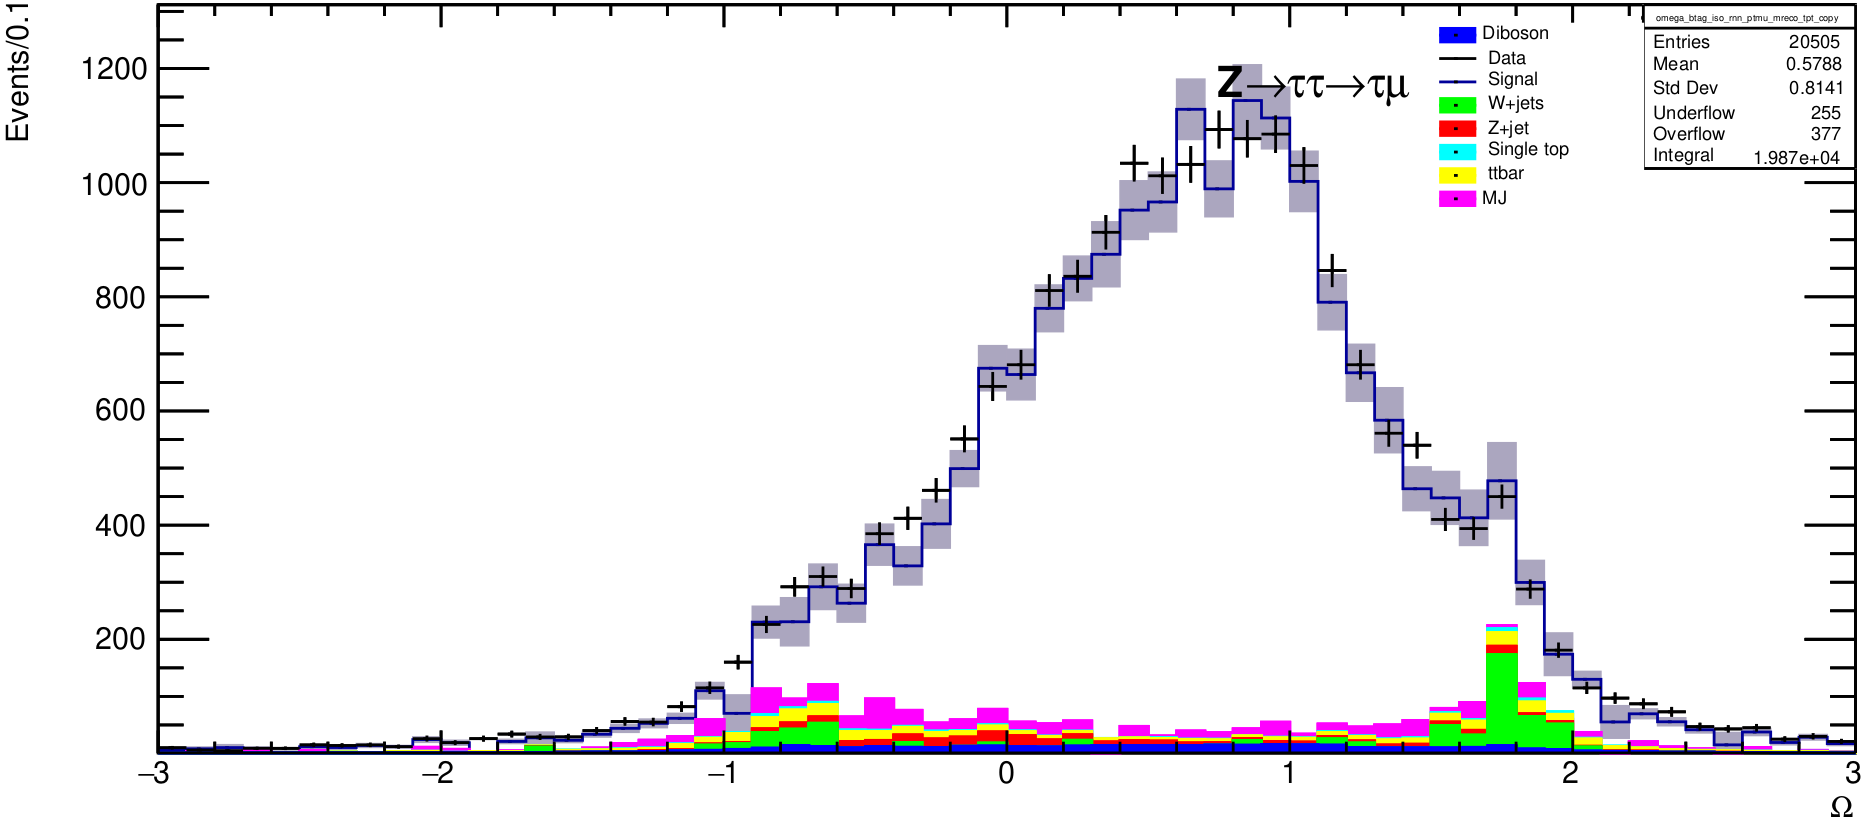
\includegraphics[width=0.7\textwidth]{figures/Fig9}
	\caption{Distribution of $\Omega$ for $Z\to\tauh\mu$ final state. }
	\label{Fig9}
\end{figure}
Adittionally, a cut on the reconstructed invariant mass ($\mreco$) of the event is made, the cut aims to pick events where the invariant mass is around the Z boson mass ($70\leq\mreco\leq 110$ GeV). The invariant mass of the final states is calculated depending on the event topology. For events where $\Omega\in [0,1]$ (\textit{in between events}),  $\mreco^{2}=(q_l+q_{\tauh}+q_{\nu_l}+q_{\nu_{\tauh}})^2$ and when the $\ptmiss$ is outside (\textit{outside events}), $(\mreco-5)^{2}=(q_l+q_{\tauh}+q_\nu)^2$. In the latter case we manually add 5 GeV to maintain our cuts consistent, since in this region the Z mass is underestimated. Fig.\ref{Fig10} shows the distribution of $\mreco$ for the in between and outside $Z\to\tauh\mu$ events. 
\begin{figure}[ht]
	\centering
	\subfloat[]{\label{Fig10a}{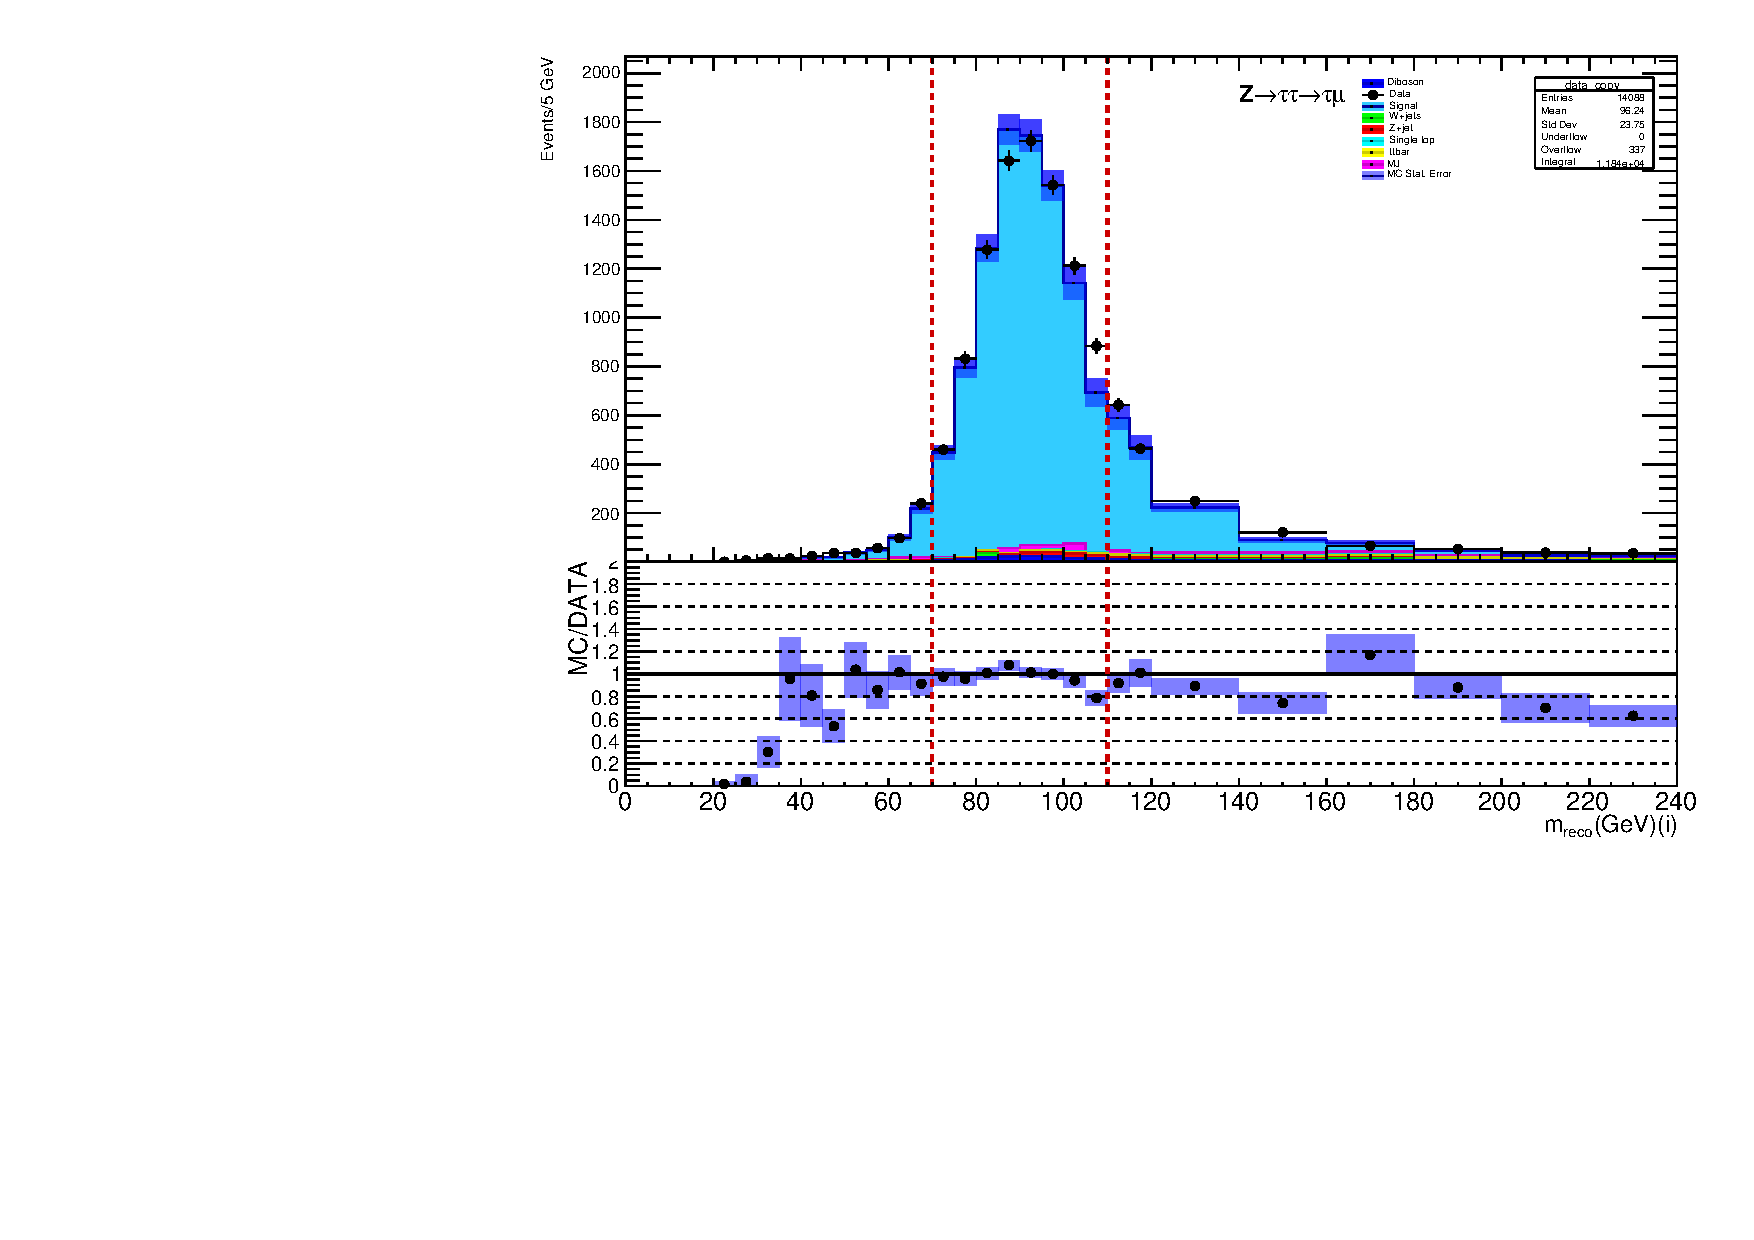
\includegraphics[width=0.50\textwidth]{figures/Fig10a}}}\hfill
	\subfloat[]{\label{Fig10b}{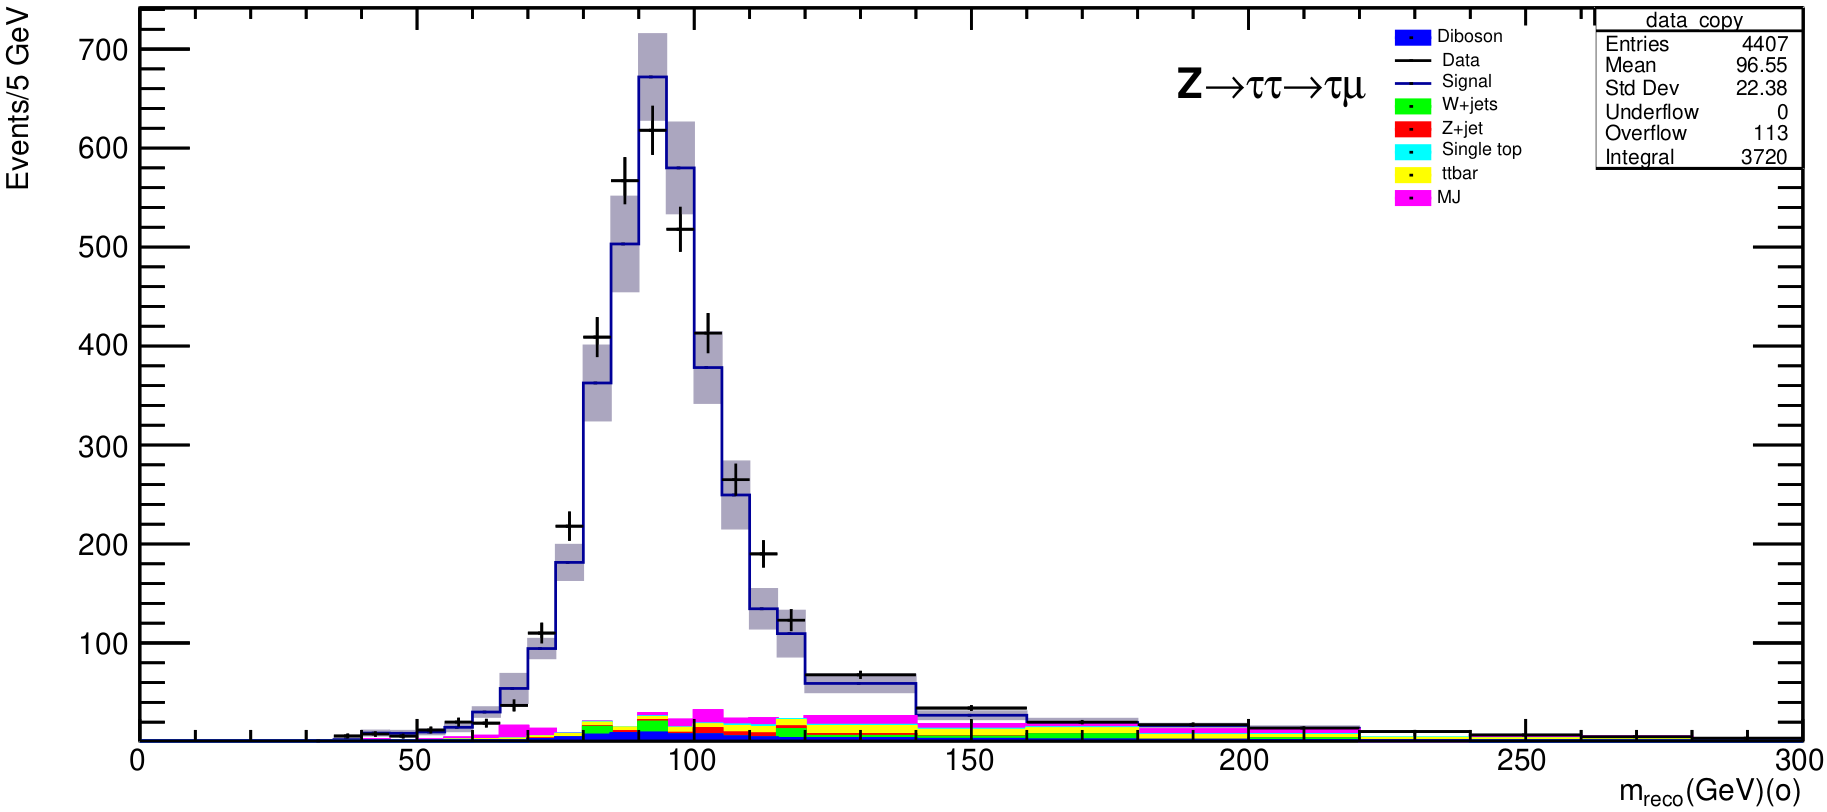
\includegraphics[width=0.50\textwidth]{figures/Fig10b}}}
	\caption{$\mreco$ distribution for the in between region (a) and the outside region (b).}
	\label{Fig10}
\end{figure}

In addition, for the $Z\to\tauh e$ final state, we add two cuts aimed to reject events where the $\tauh$ candidate is faked by an electron. First to reject $Z\to ee$ events, a requirement on the invariant mass of the electron and $\tauh$ candidate is made, $m(e,\tauh)<80$ GeV. Then, we also make use of an ID algorithm trained to discriminate electrons from real $\tauh$. In our case, eBDTScore$\geq 0.06$. The distributions for this variables are shown in Fig.\ref{Fig11}.
\begin{figure}[ht]
	\centering
	\subfloat[]{\label{Fig11a}{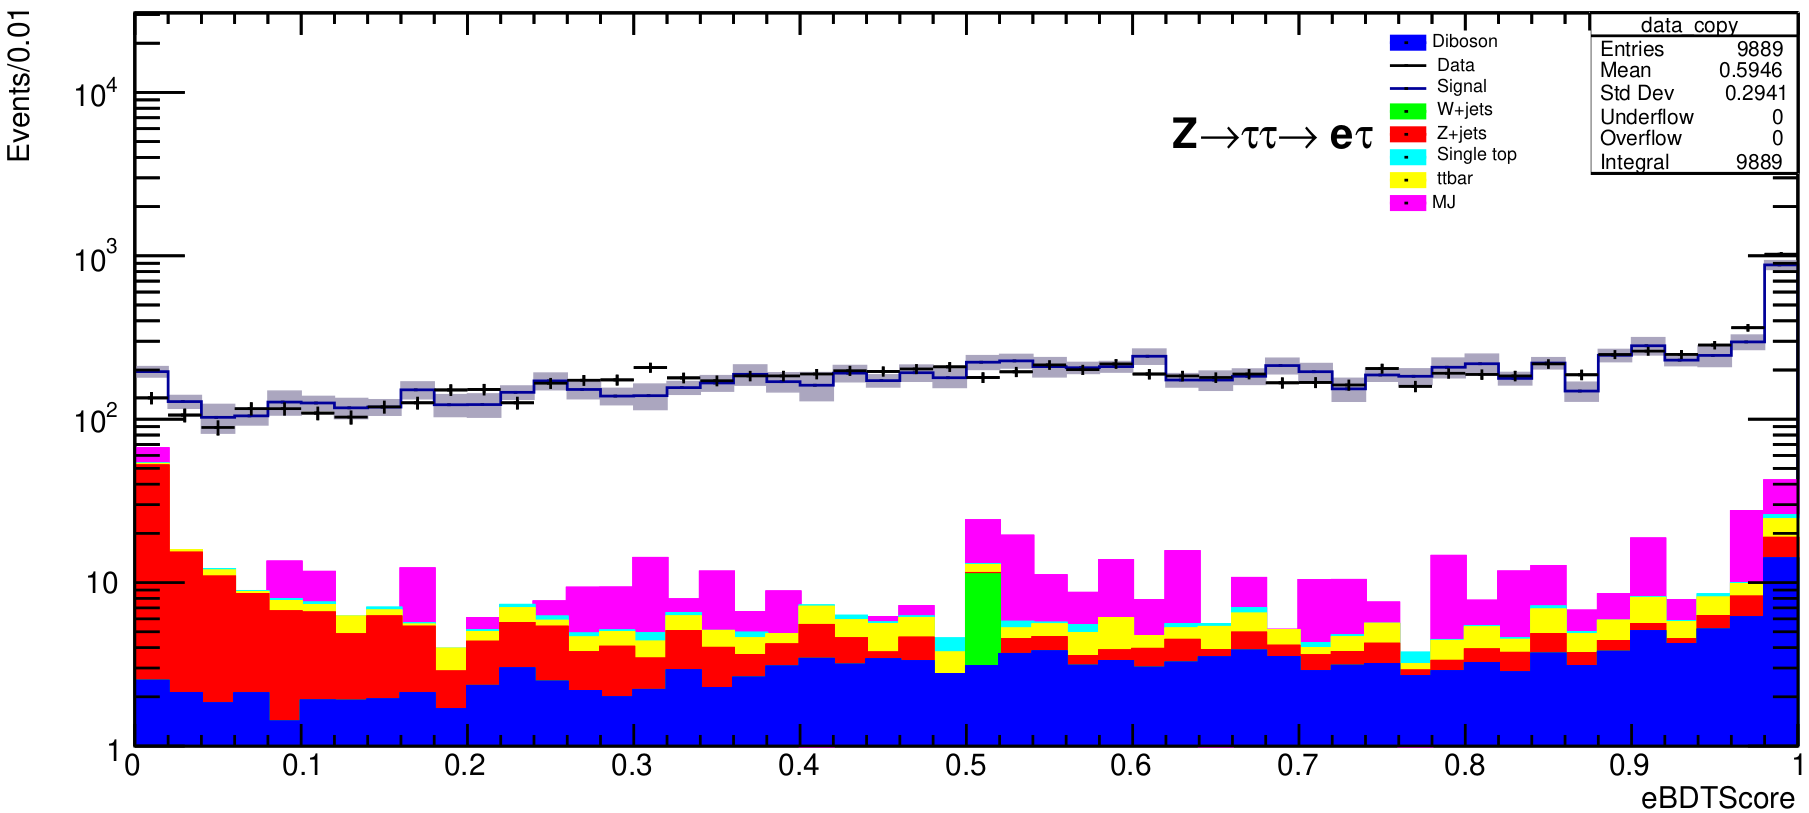
\includegraphics[width=0.50\textwidth]{figures/Fig11a}}}\hfill
	\subfloat[]{\label{Fig11b}{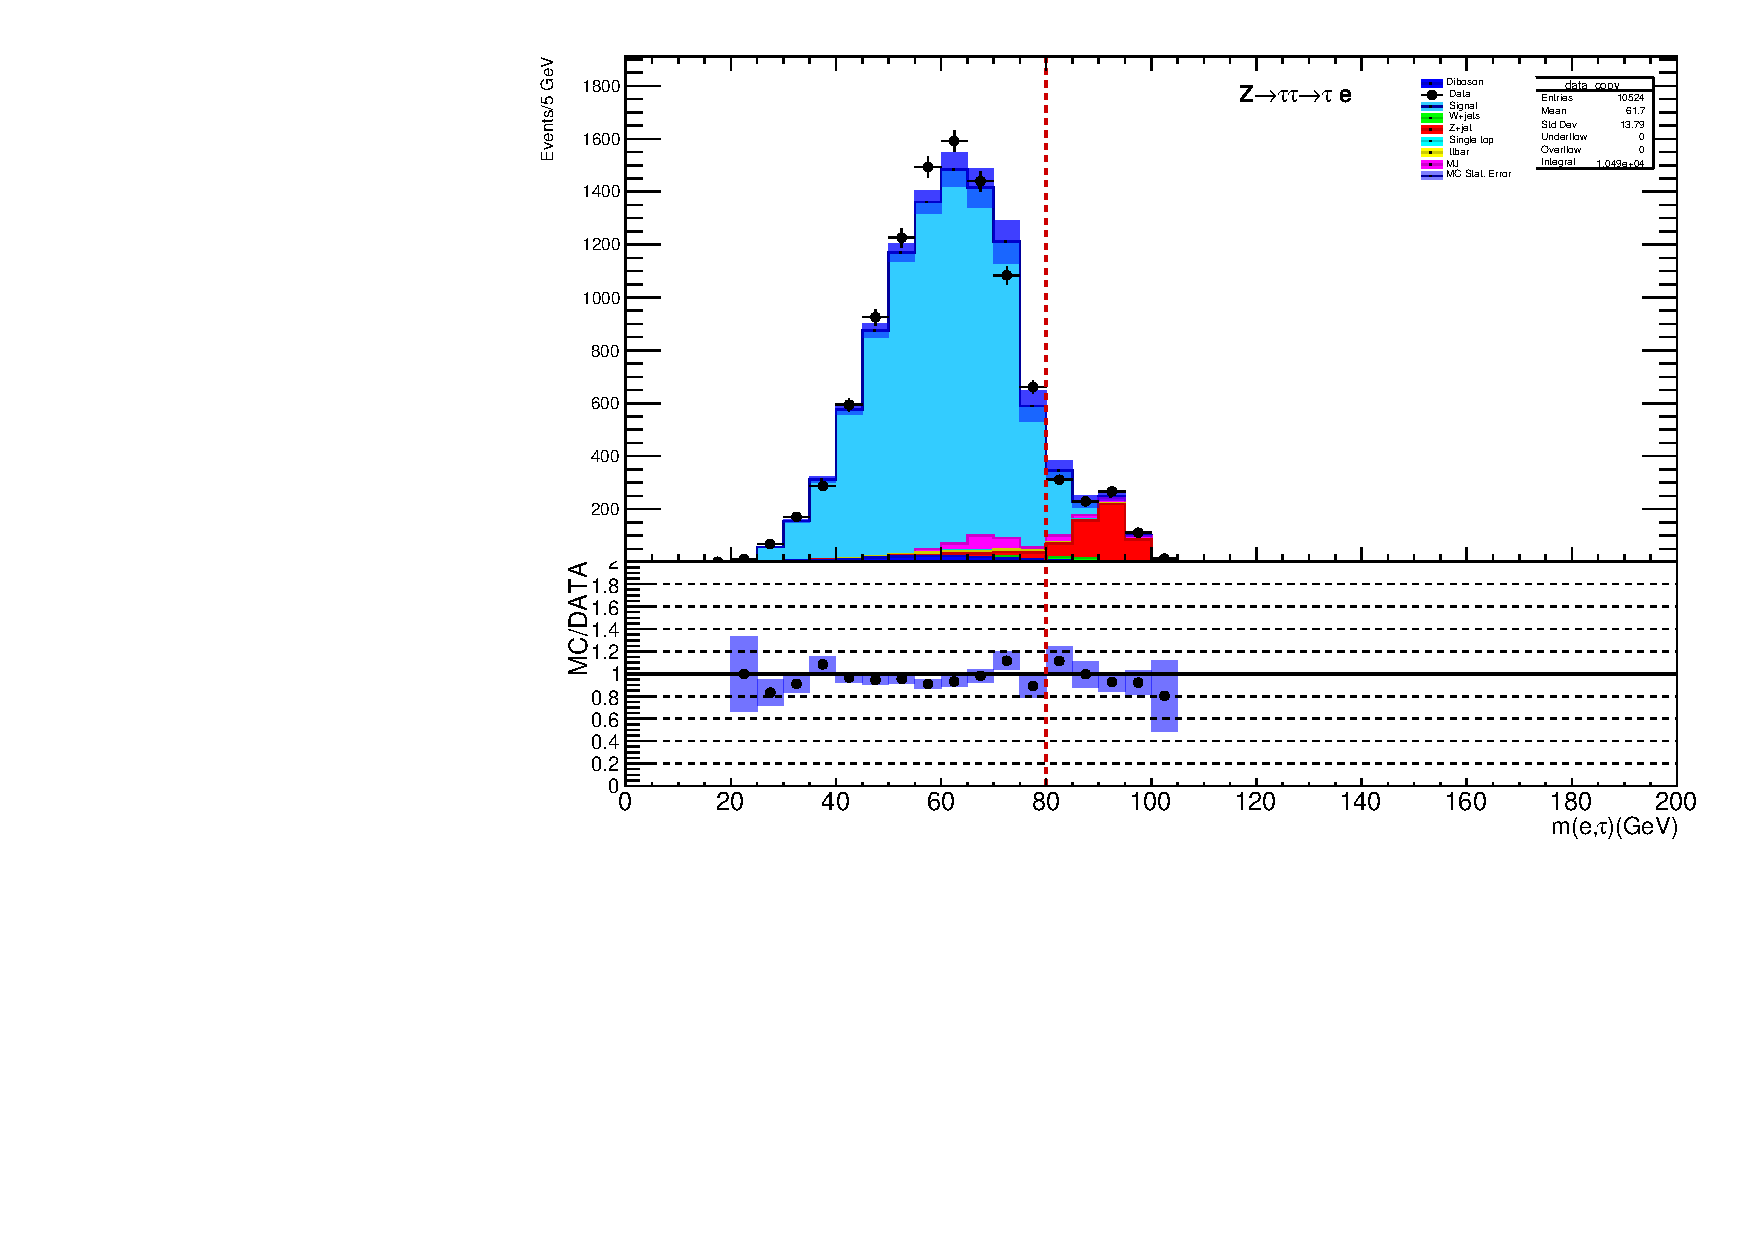
\includegraphics[width=0.50\textwidth]{figures/Fig11b}}}
	\caption{Distribution of the variables used for rejecting $\tauh$ fakes coming from electrons. On the right $m(e,\tauh)$ distribution (a) and on the left the eBDTScore distribution (b).}
	\label{Fig11}
\end{figure}
Finally, in order to measure the tau ID scale factors on the high-$p_T$ region we select events where $p_T(\tauh)\geq 45$ GeV. The $p_T$ distributions for $\tauh$ candidates are shown in Fig.\ref{Fig12} for the in between and outside regions.
\begin{figure}[ht]
	\centering
	\subfloat[]{\label{Fig12a}{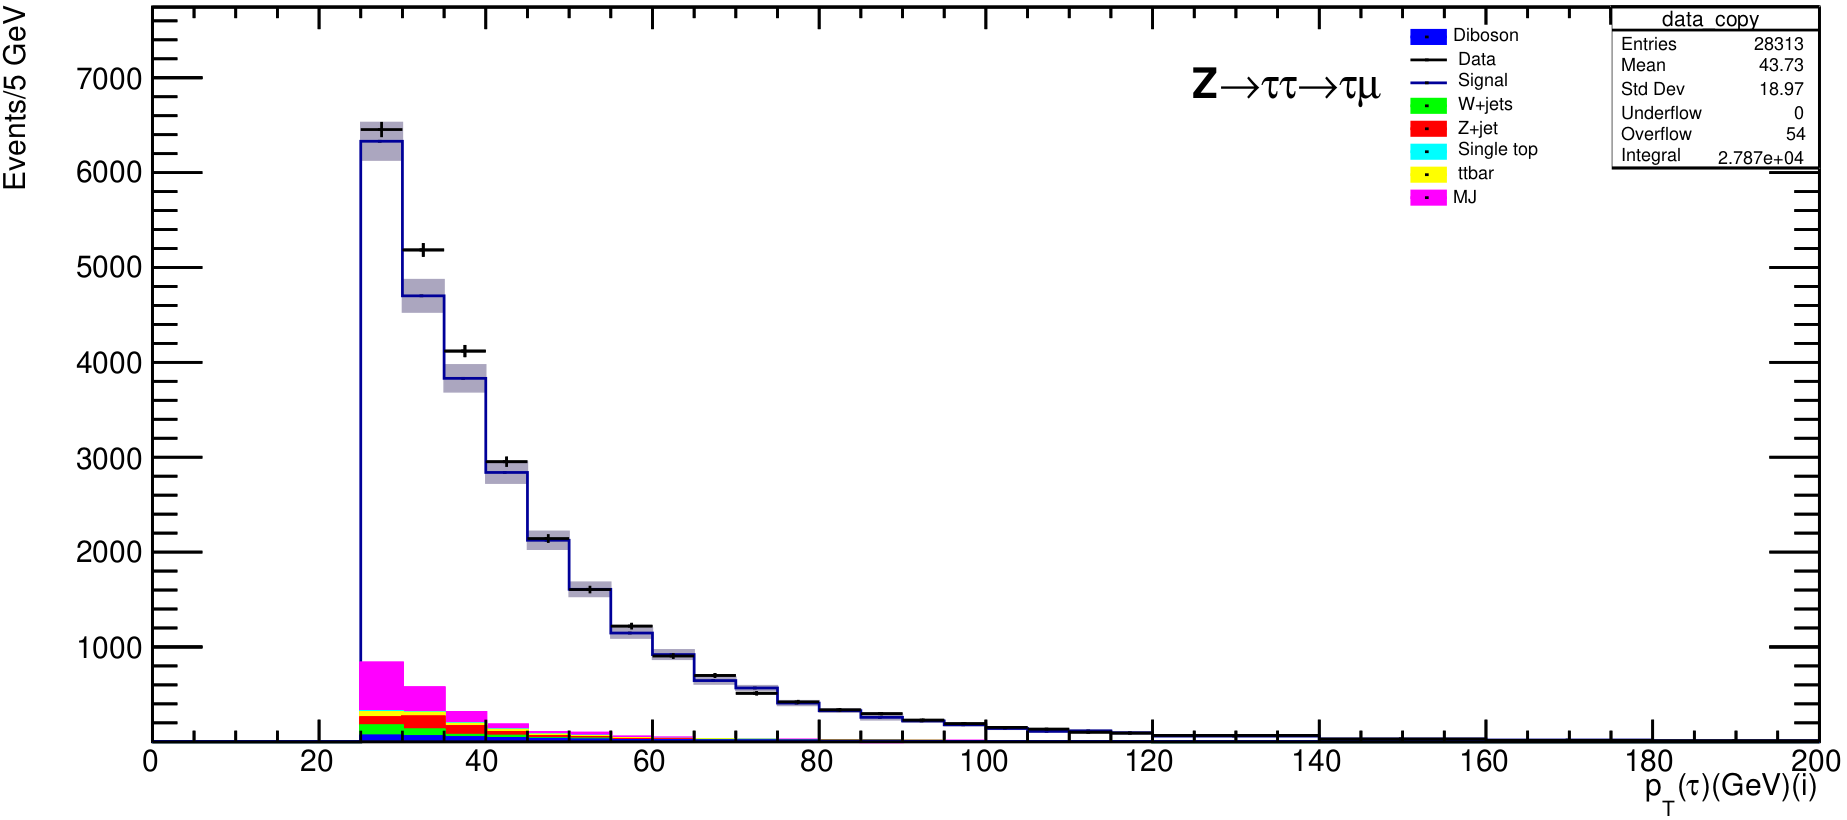
\includegraphics[width=0.50\textwidth]{figures/Fig12a}}}\hfill
	\subfloat[]{\label{Fig12b}{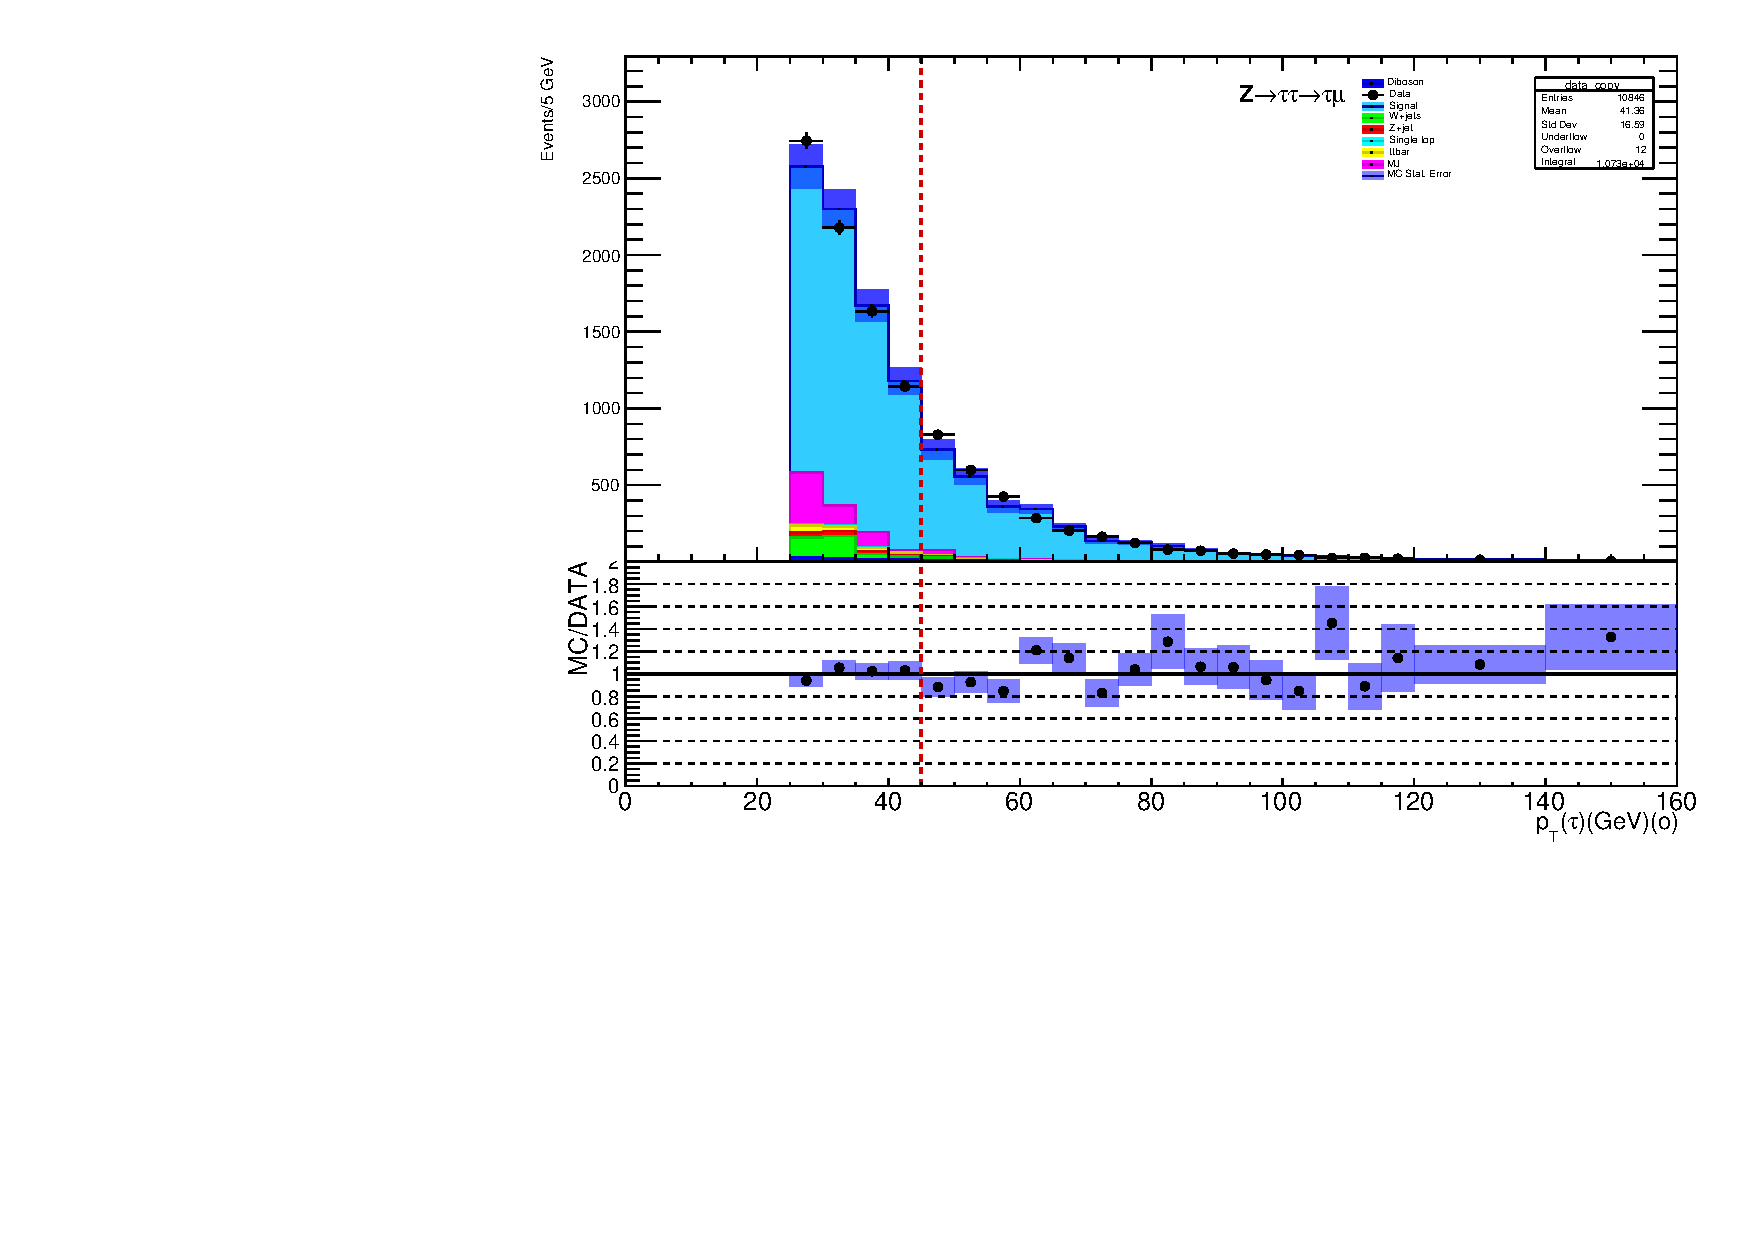
\includegraphics[width=0.50\textwidth]{figures/Fig12b}}}
	\caption{$p_T(\tauh)$ distribution for the in between (a) and outside (b) regions.}
	\label{Fig12}
\end{figure} 
\section{Multi Jet Background Estimation}
As we said previously, $\tauh$ candidates are seeded by jets, thus, QCD events represent a source of background. Nonetheless, we do not have MC simulations for this processes as compared with the EW interactions shown in Table \ref{Table3}. For this reason, we use a \textit{data driven method} to estimate multi jet (MJ) background. For that purpose, we choose a variable that in principle we suppose is uncorrelated with the shape of the MJ background. For our study, this variable is the relative sign between the charges of the $\tauh$ and the lepton. Thus, this defines two regions: the same sign (SS) region where $q(\tauh)=q(l)$ and the opposite sign region where $q(\tauh)=-q(l)$. Our estimate of MJ background for the SS region is obtained subtracting signal and electroweak backgrounds (EWBG) simulated contributions, basically:
\begin{equation}
\text{MJBG}_{\text{SS}}=\text{Data}_{\text{SS}}-\text{Signal}_{\text{SS}}-\text{EWBG}_{\text{SS}},
\end{equation}
 To study the residual charge correlation, we define a control region (CR) where the MJ background is enhanced. This region is defined by events that fail either the lepton isolation criteria or the $\tauh$ ID requirement of tauRNNScore$>0.4\, (0.55)$ for 1-prong (3-prong) $\tauh$ candidates and have the same other kinematic features of the signal region (SR) described in section \ref{chap4sec3}. A diagram showing the four regions just defined is shown in Fig.\ref{Fig13}. Now, if charge correlation is the same in SR and CR, we have:
 \begin{equation}
 \frac{\text{MJBG}_{\text{SROS}}}{\text{MJBG}_{\text{SRSS}}}=\frac{\text{MJBG}_{\text{CROS}}}{\text{MJBG}_{\text{CRSS}}},
 \end{equation}
then,
 \begin{equation}
\text{MJBG}_{\text{SROS}}=\text{MJBG}_{\text{SRSS}}\times \text{RQCD}\,
\label{eq36}
\end{equation}
where $\text{RQCD}\equiv\frac{\text{MJBG}_{\text{CROS}}}{\text{MJBG}_{\text{CRSS}}}$. So, \eqref{eq36} gives the estimation of MJ background on the signal region (SROS).
\begin{figure}[h]
	\centering
	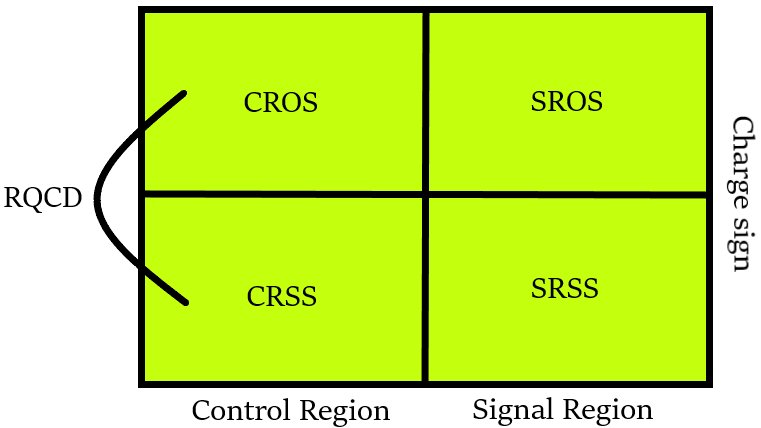
\includegraphics[width=0.5\textwidth]{figures/Fig13}
	\caption{Diagram showing the regions defined to estimate MJ background contribution in the SROS region. This data-driven method is also known as ABCD method.}
	\label{Fig13}
\end{figure}
 
    \chapter{Results}\label{chap5}
In this section we present the preliminary results of the performance of the $\tauh$ identification algorithm using $\int\mathcal{L} dt=139.2$ fb$^{-1}$ of data recorded between 2015 and 2018.
The correction factors are applied to simulation in order to match the efficiency observed in data. These correction factors are defined as the ratio between the efficiency measured in data and in simulation.
\begin{equation}
C_{\text{ID}}=\frac{\mathcal{E}_{\text{Data}}}{\mathcal{E}_{\text{MC}}}.
\end{equation}
For this work, we present a preview of the value of the correction factors for \textit{Tight} ID working point for $\tauh$ candidates with $\pt$ above 45 GeV. Since this report is about a work in progress and we have not studied yet the effect of the systematic uncertainties on our results, we will take another approach on estimating the correction factors.

\section{Systematic uncertainties}
The values for the systematic uncertainties used to report the value of the correction factors are presented in Table \ref{Tab5}. These numbers have been provided by Terry Wyatt and Sam Dysch, based on their previous experience working on analysis that make use of $Z\to\tauh l$ events on a similar phase space.
\begin{table}[]
	\centering
	\begin{tabular}{cc}
		\hline
		\multicolumn{1}{|c|}{Source}        & \multicolumn{1}{c|}{Sys. Uncertainty (\%)} \\ \hline
		Electron ID efficiency              & 0.8                                        \\
		Muon ID Efficiency                  & 0.2                                        \\
		Electron $\pt$ scale and resolution & 0.4                                        \\
		Muon $\pt$ scale and resolution     & 0.3                                        \\
		Tau $\pt$ scale                     & 1.9                                        \\
		Electron trigger efficiency         & 0.1                                        \\
		Muon trigger efficiency             & 0.4                                        \\ 
		Integrated luminosity               & 1.7                                        \\ \hline
	\end{tabular}
	\caption{Systematic uncertainties used in this study.}
	\label{Tab5}
\end{table}
\section{$\mu\tau$ Final state}
We define the simulation correction factor as
\begin{equation}
	C_{\text{Tight-ID}}=\frac{N_{\text{Data}}}{N_{\text{MC}}}.
\end{equation}
Where N is the total number of events that pass our selection. The value obtained for the final state that contains one muon and a $\tauh$ candidate is

All the distributions of the relevant cuts for selecting our signal events after applying all the other cuts are shown in Fig.\ref{Fig17} (Appendix A).
\section{$e\tau$ Final state}
The value obtained for $C_{\text{Tight-ID}}$ in the final state that contains one electron and a $\tauh$ candidate is

All the distributions of the relevant cuts for selecting our signal events after applying all the other cuts are shown in Fig.\ref{Fig18} (Appendix A).
\section{Discussion}
As this study makes use of events highly boosted on the transverse plane the Z$(\pt)$ modelling is very important. In the first stages of our analysis we used Powheg+Pythia8 to simulate $Z\to\tauh l$ events. Fig.\ref{Fig23} shows the Z$(\pt)$ and $\Delta\phi(\tauh,l)$ for the muon-tau final state for in between events. As it can be seen the tendency in the MC is to underestimate the data for high-Z$(\pt)$ values. These results have been previously reported by ATLAS studies \cite{Aad:2019wmn}, and Fig.\ref{Fig20} shows the Z$(\pt)$ modelling made by different generators. This has motivated us to use Sherpa to simulate our signal events. The Z$(\pt)$ results for this generator are shown in Fig.\ref{Fig19} and there is improvement for high-$\pt$ values over Powheg+Pythia8. The complete set of plots showing the Z$(\pt)$ distribution for both e-tau and mu-tau final states for the two different type of topologies are shown in Fig.\ref{Fig21} and Fig.\ref{Fig22}.
\begin{figure}[ht]
	\centering
	\subfloat[]{\label{Fig23a}{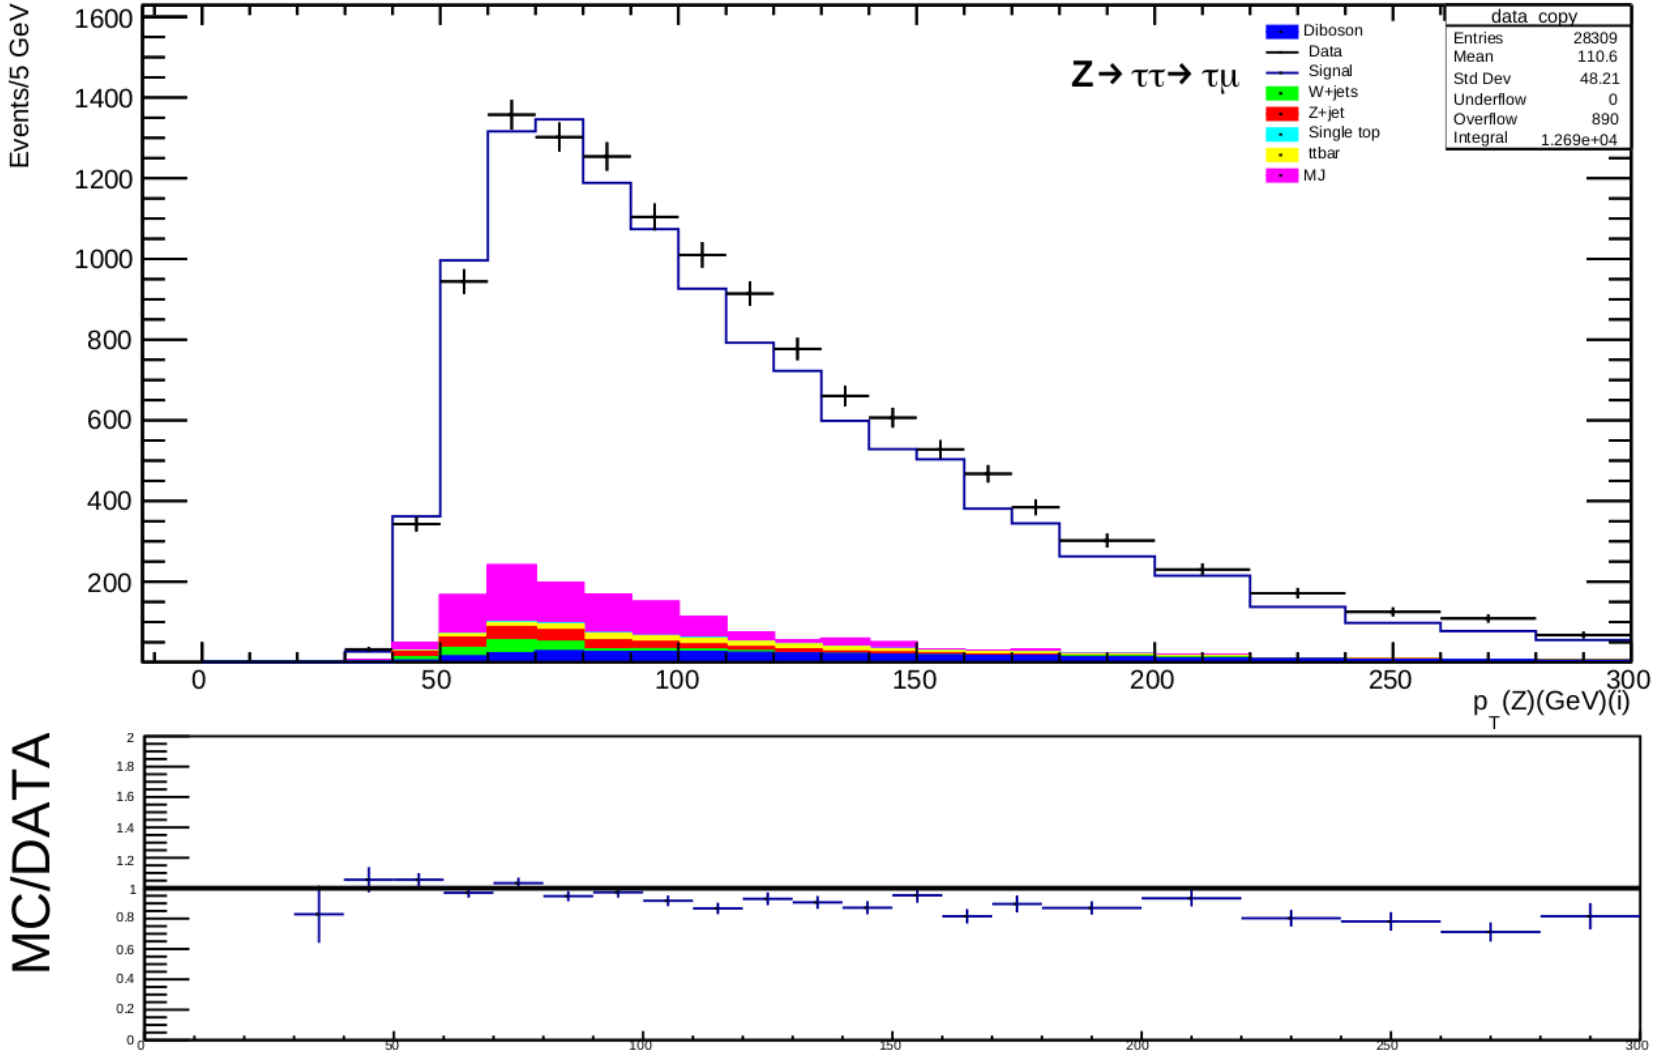
\includegraphics[width=0.50\textwidth]{figures/Fig23a}}}\hfill
	\subfloat[]{\label{Fig23b}{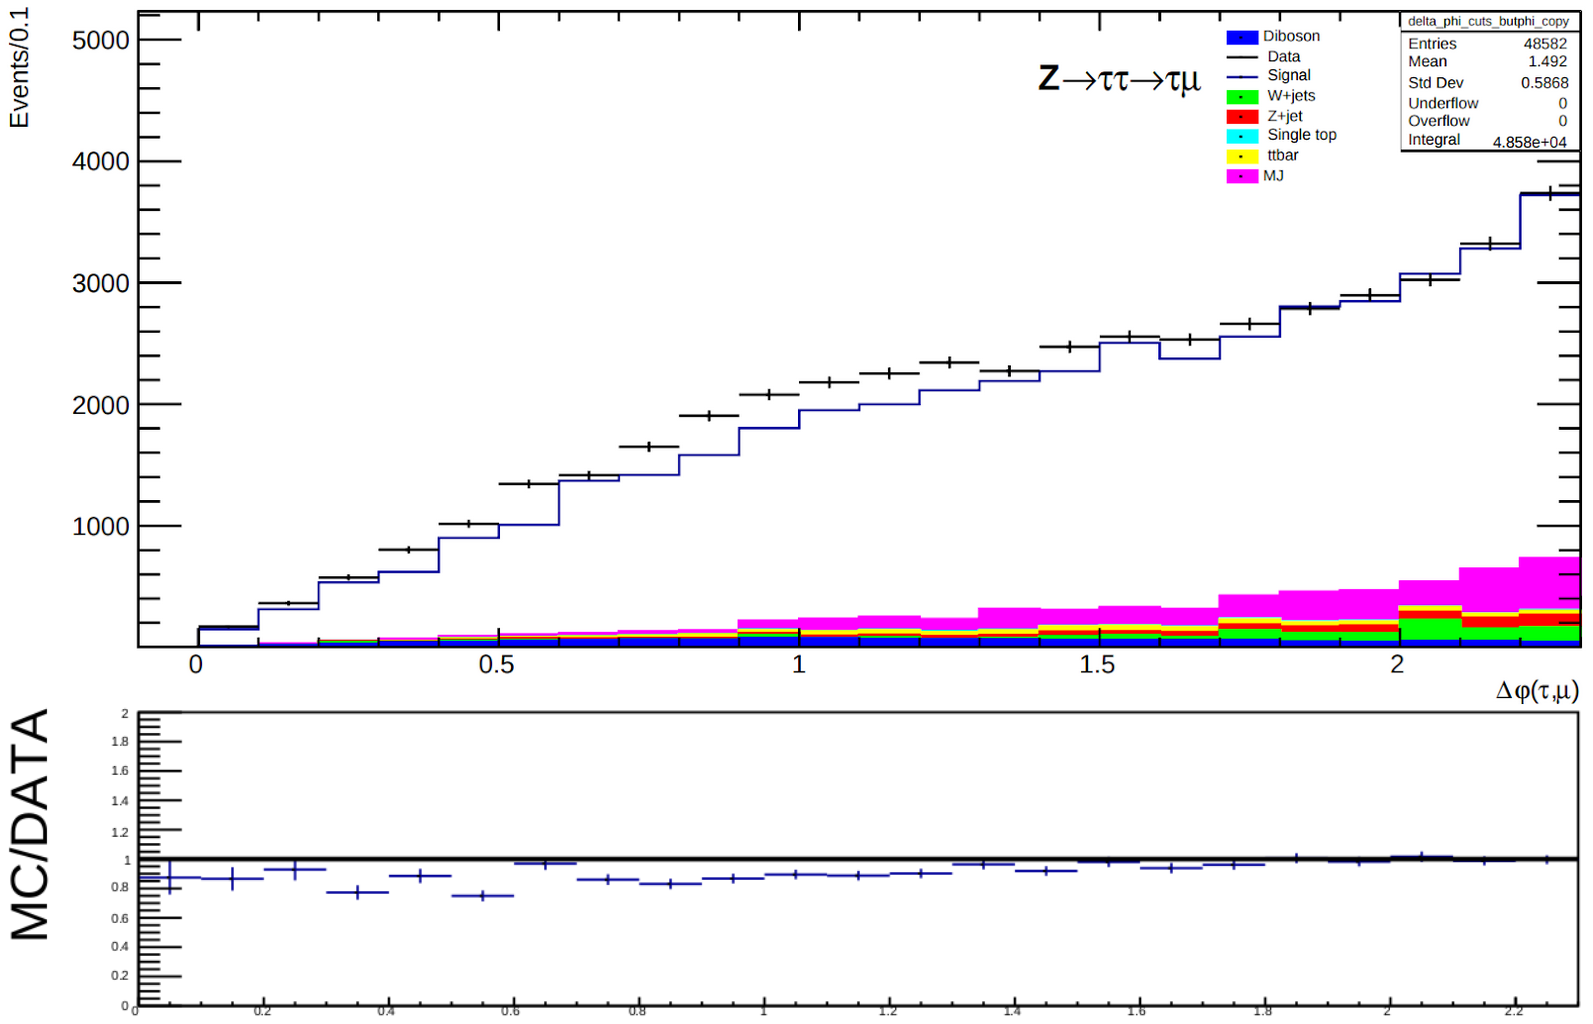
\includegraphics[width=0.50\textwidth]{figures/Fig23b}}}
	\caption{Distribution of Z$(\pt)$ for in between events (a) and $\Delta\phi(\tauh,l)$ (b) using Powheg+Pythia8. All the other cuts have been applied apart from the one being plotted.}
	\label{Fig23}
\end{figure}
\begin{figure}[ht]
	\centering
	\subfloat[]{\label{Fig19a}{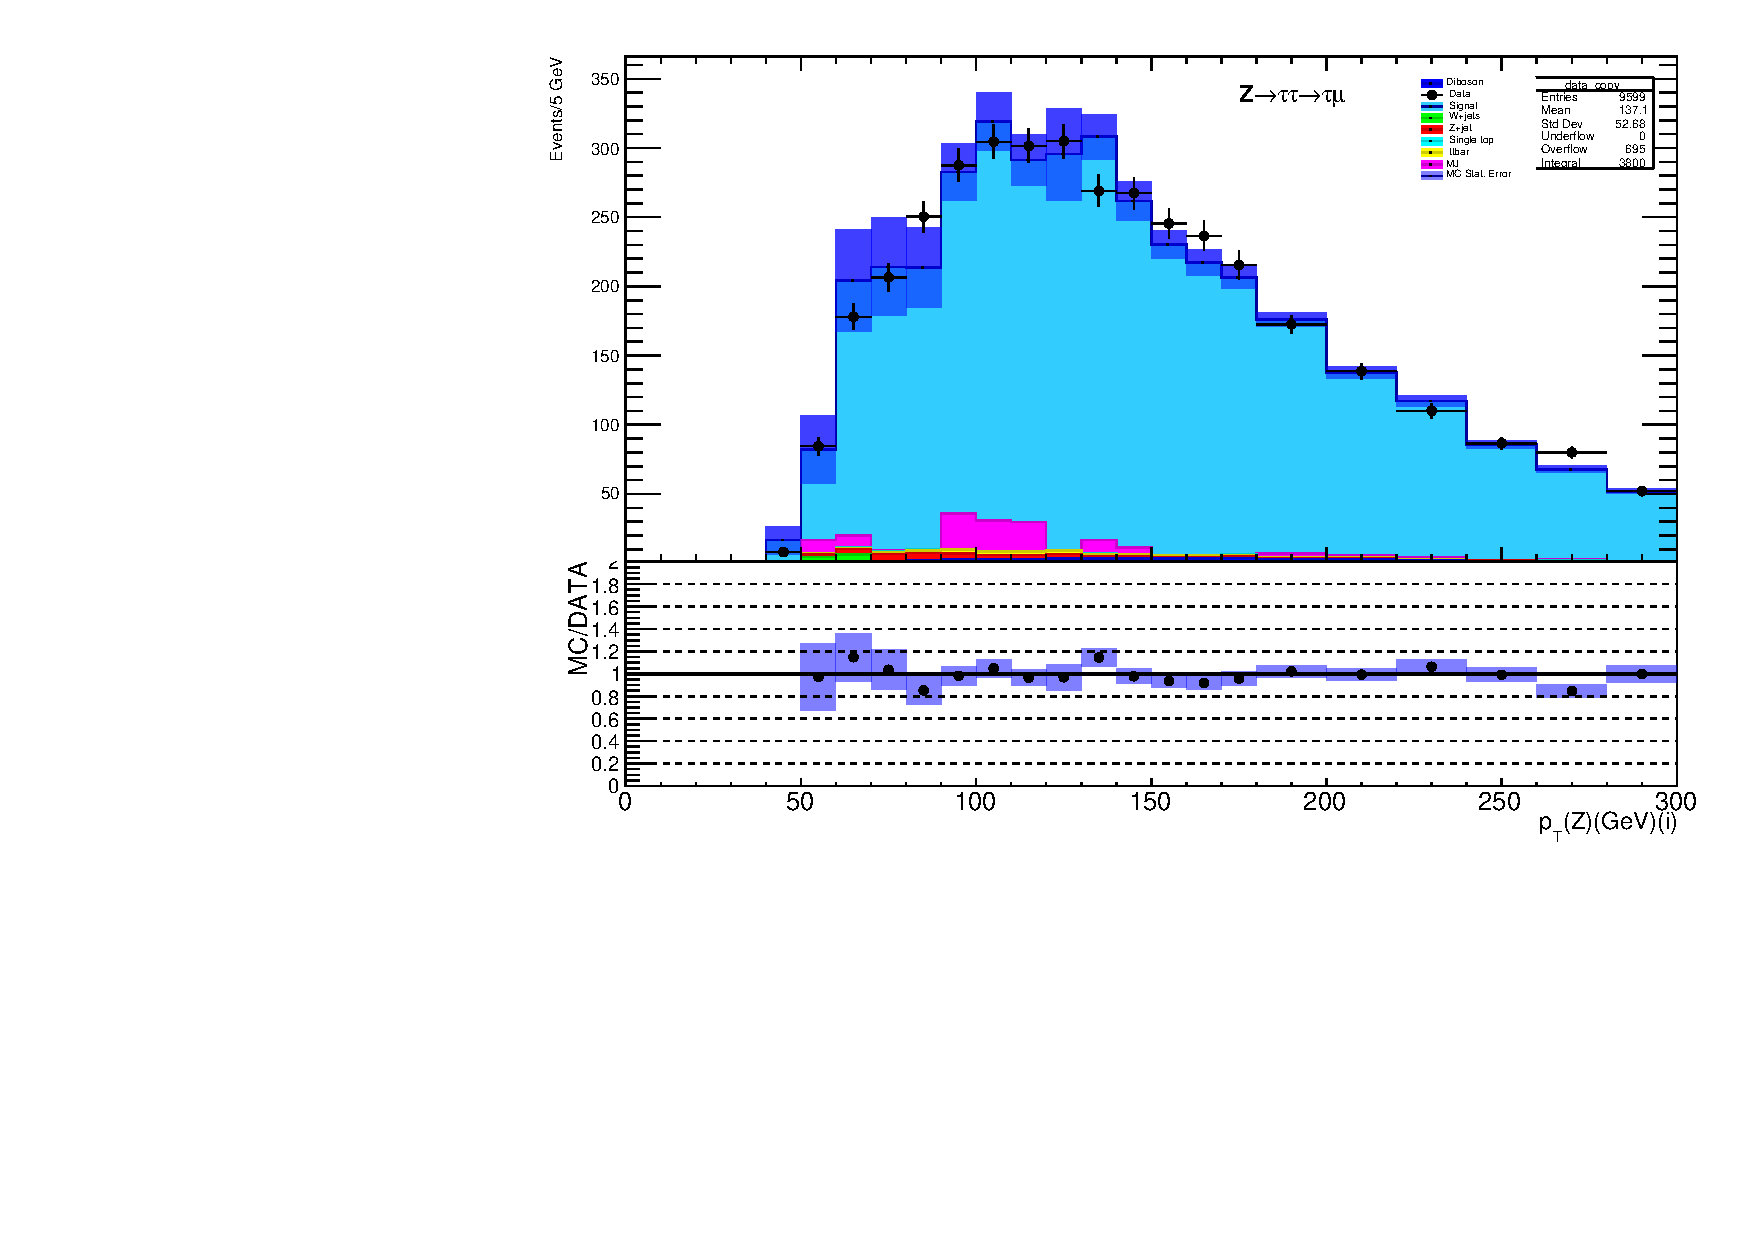
\includegraphics[width=0.50\textwidth]{figures/Fig19a}}}\hfill
	\subfloat[]{\label{Fig19b}{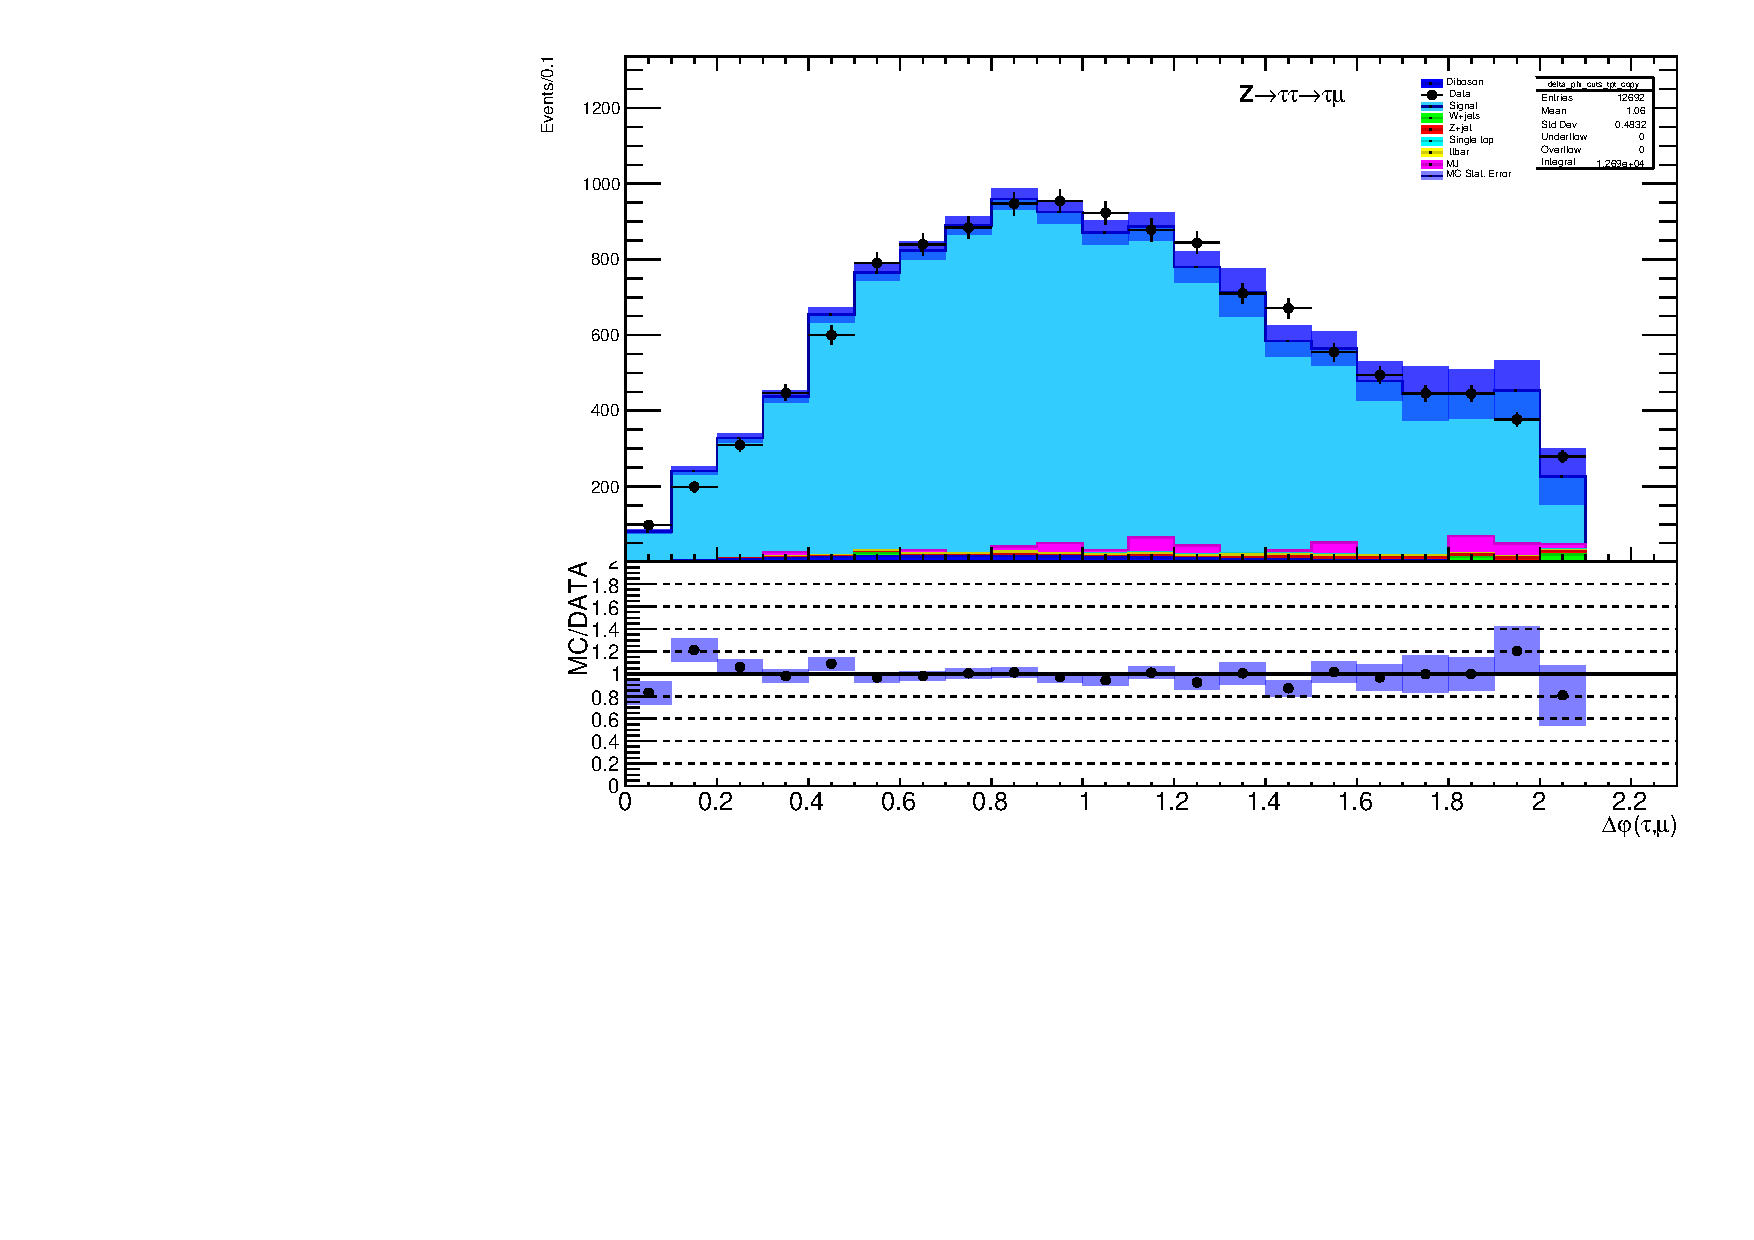
\includegraphics[width=0.50\textwidth]{figures/Fig19b}}}
	\caption{Distribution of Z$(\pt)$ for in between events (a) and $\Delta\phi(\tauh,l)$ (b) using Sherpa. All the other cuts have been applied apart from the one being plotted.}
	\label{Fig19}
\end{figure}
\begin{figure}[h]
	\centering
	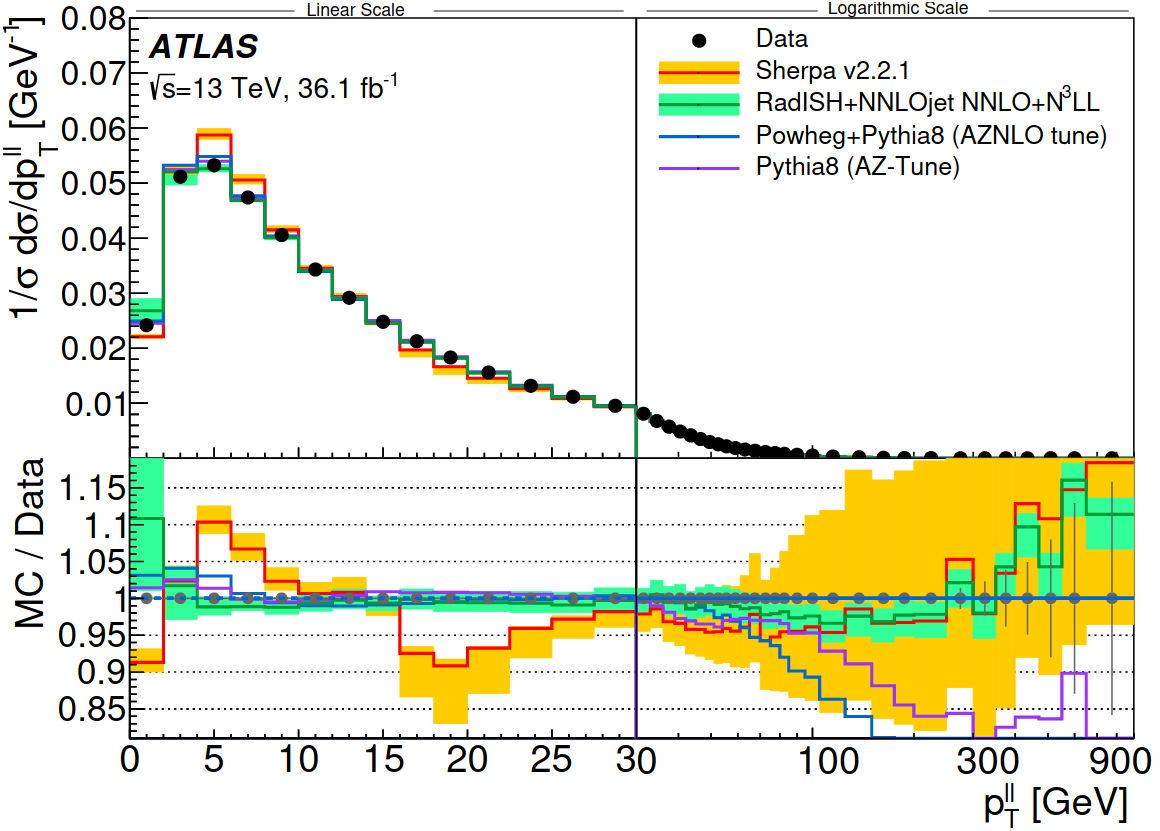
\includegraphics[width=0.5\textwidth]{figures/Fig20}
	\caption{Diagram showing the regions defined to estimate MJ background contribution in the SROS region. This data-driven method is also known as ABCD method.}
	\label{Fig20}
\end{figure}

Another challenging 
    \chapter{Conclusions and prospects}\label{chap6}

    \appendix
\chapter{Appendices}
\section{$Z\to\tauh\mu$ final state distributions}
\begin{figure}[ht]
	\centering
	\subfloat[]{\label{Fig17a}{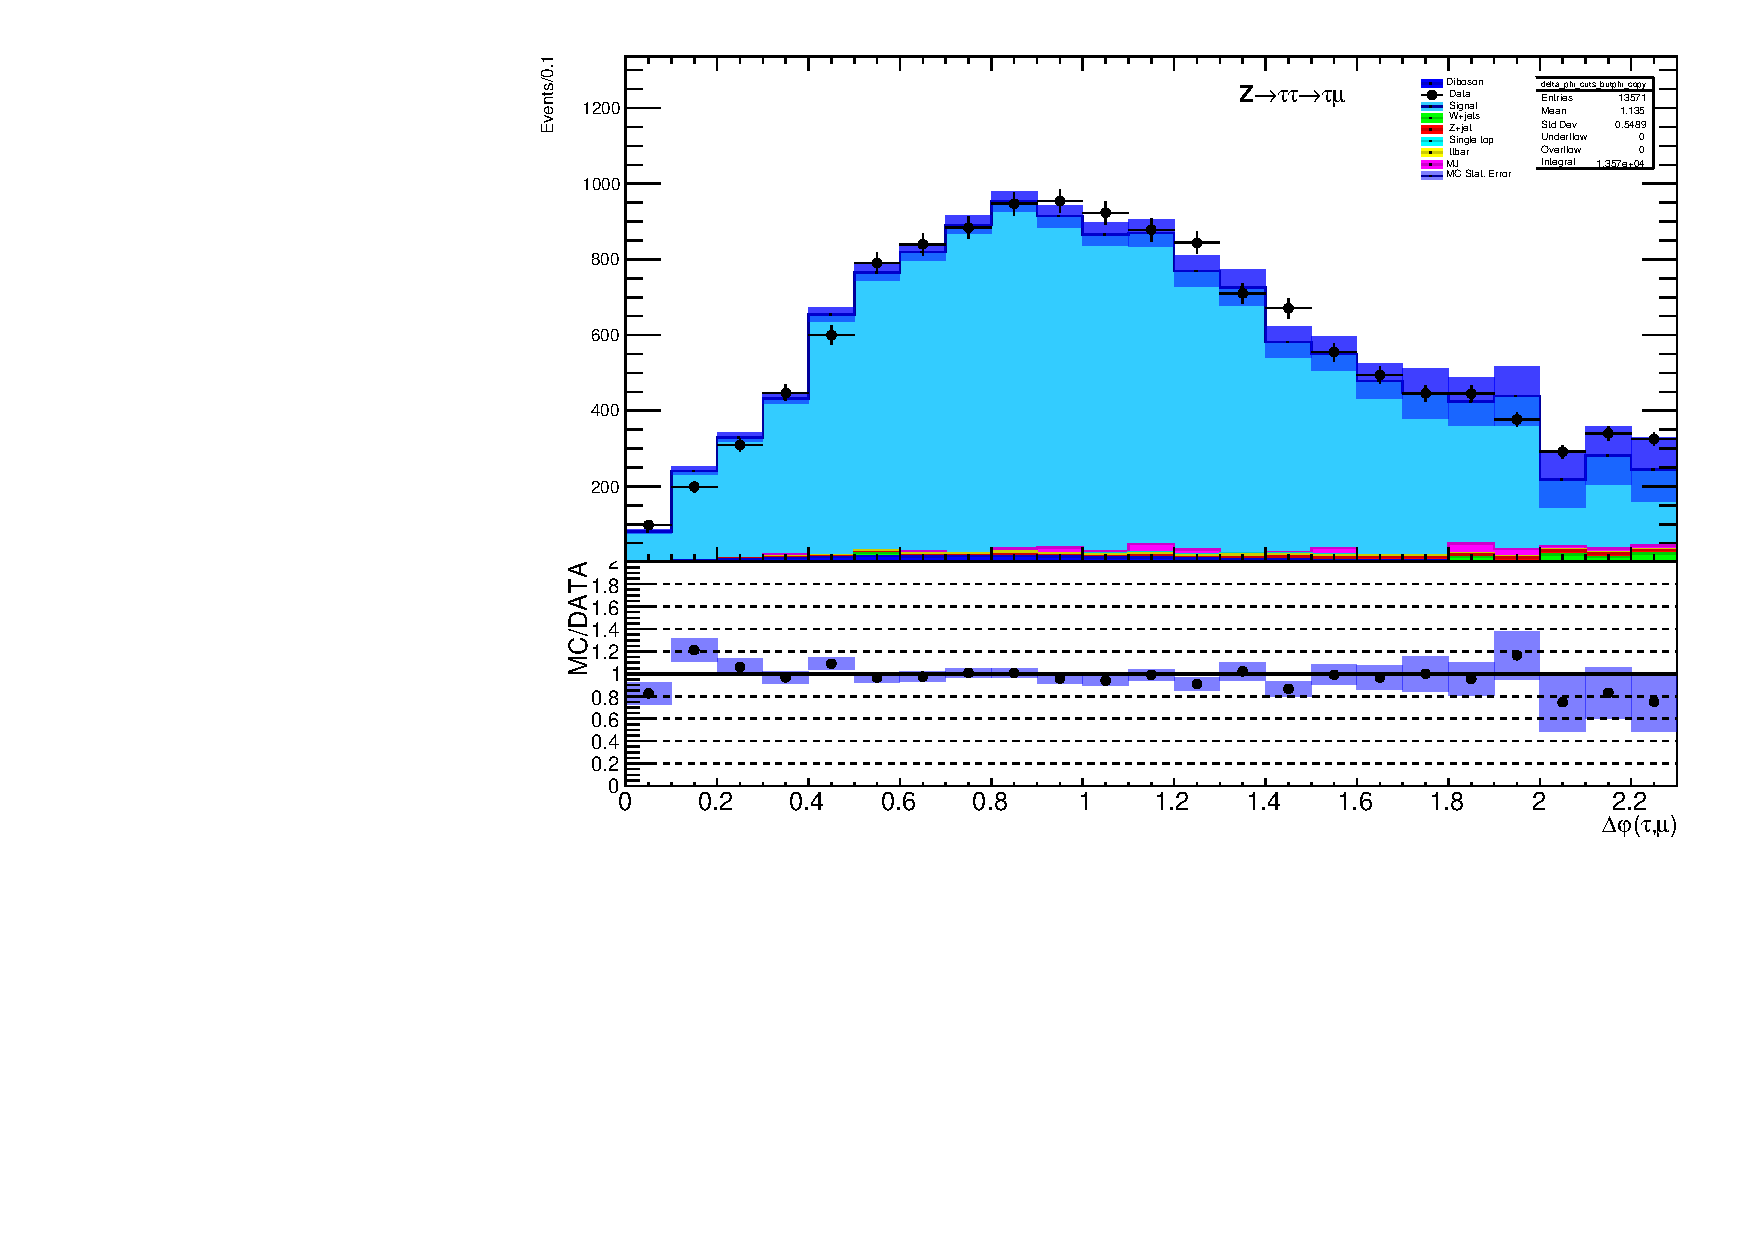
\includegraphics[width=0.50\textwidth]{figures/Fig17a}}}\hfill
	\subfloat[]{\label{Fig17b}{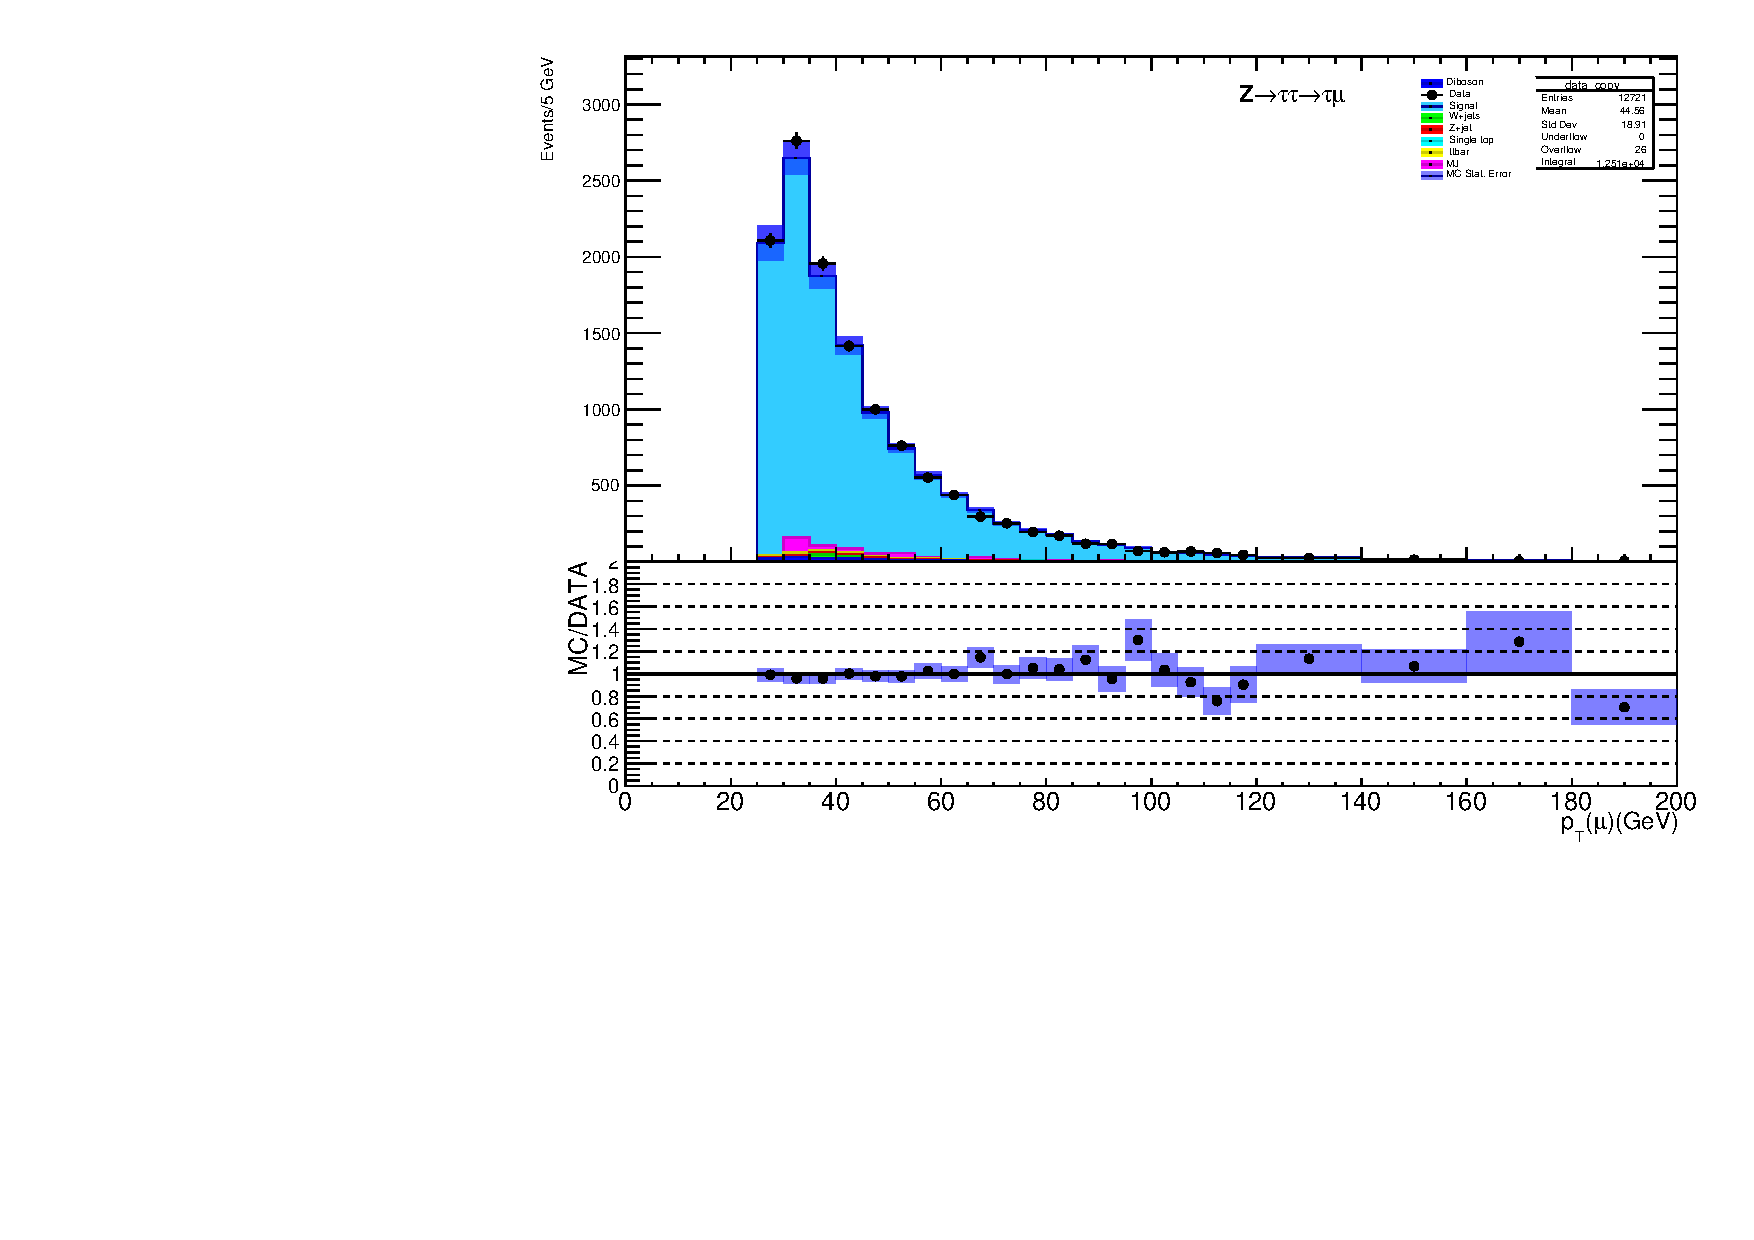
\includegraphics[width=0.50\textwidth]{figures/Fig17b}}}\hfill
	\subfloat[]{\label{Fig17c}{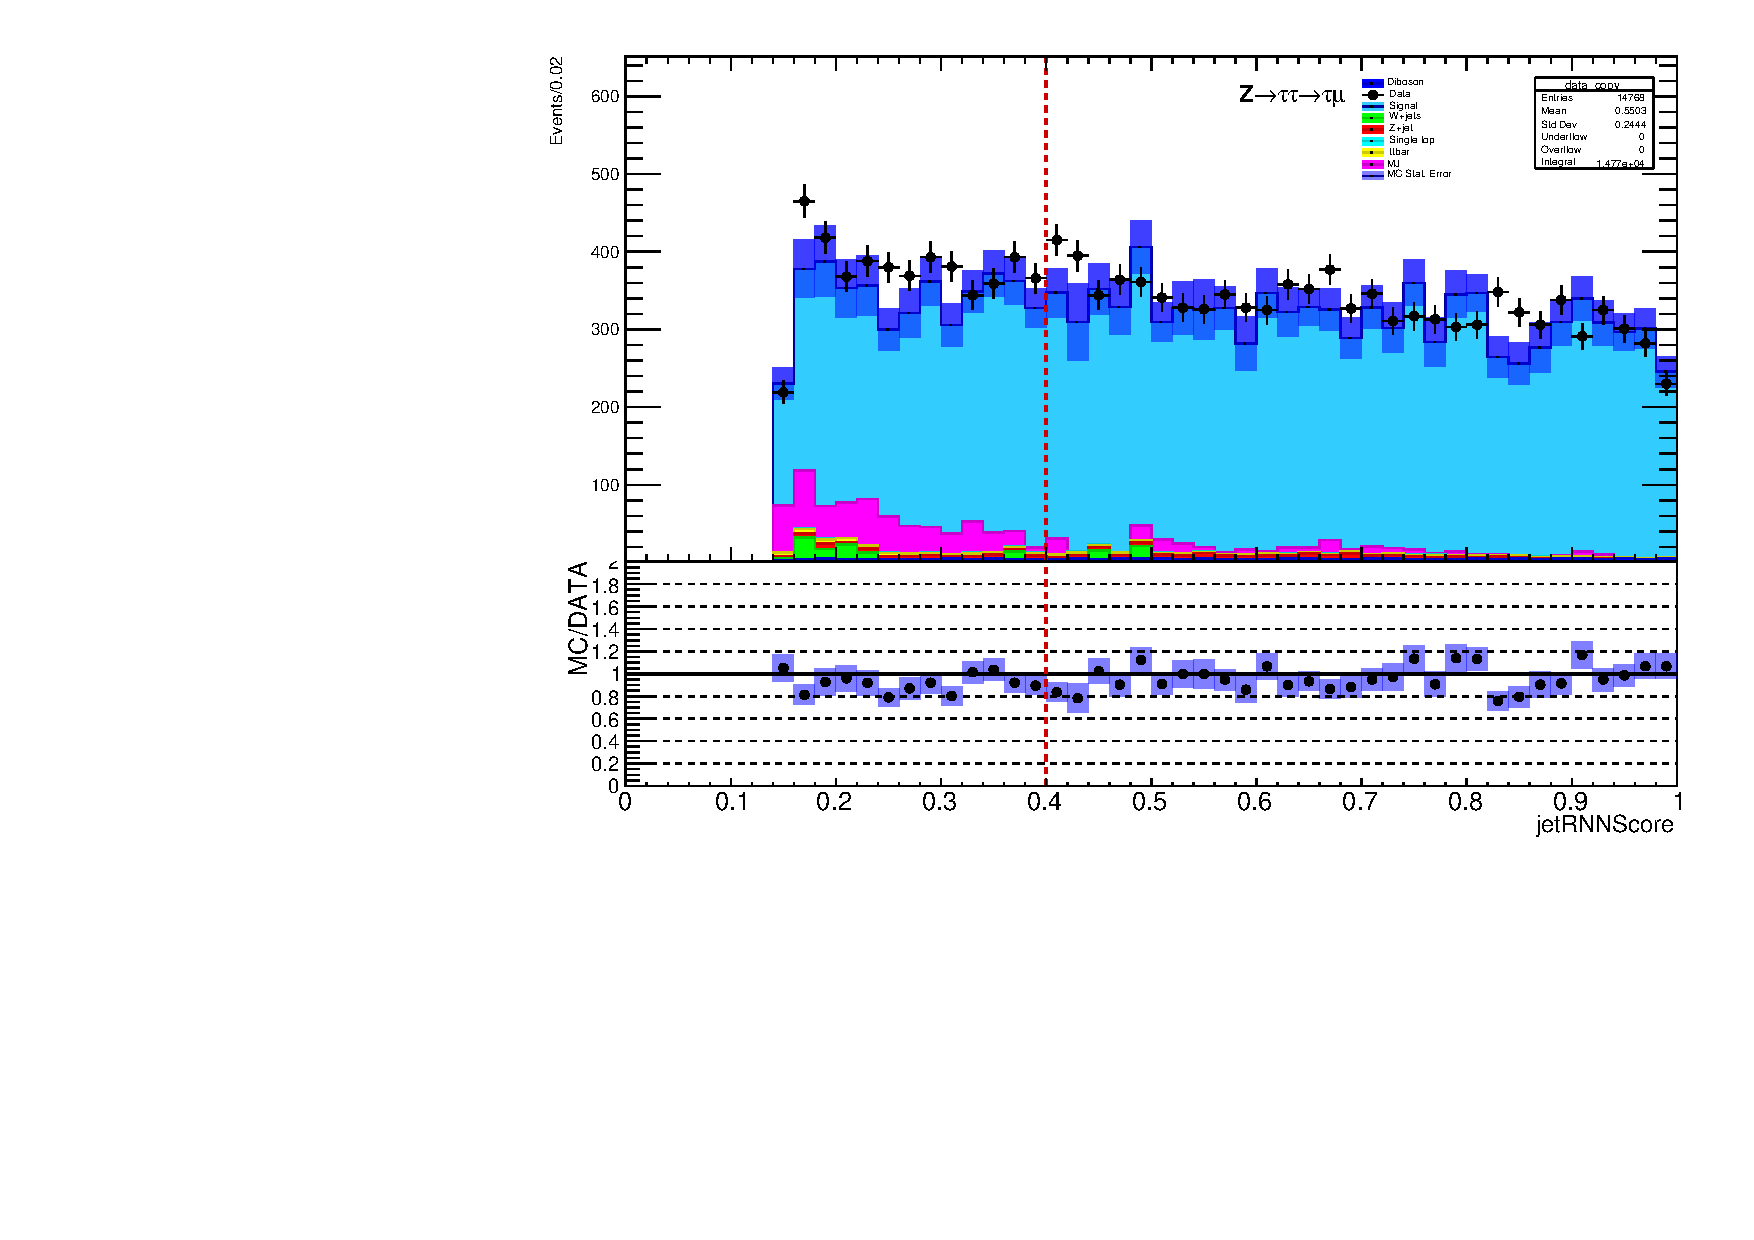
\includegraphics[width=0.50\textwidth]{figures/Fig17c}}}\hfill
	\subfloat[]{\label{Fig17d}{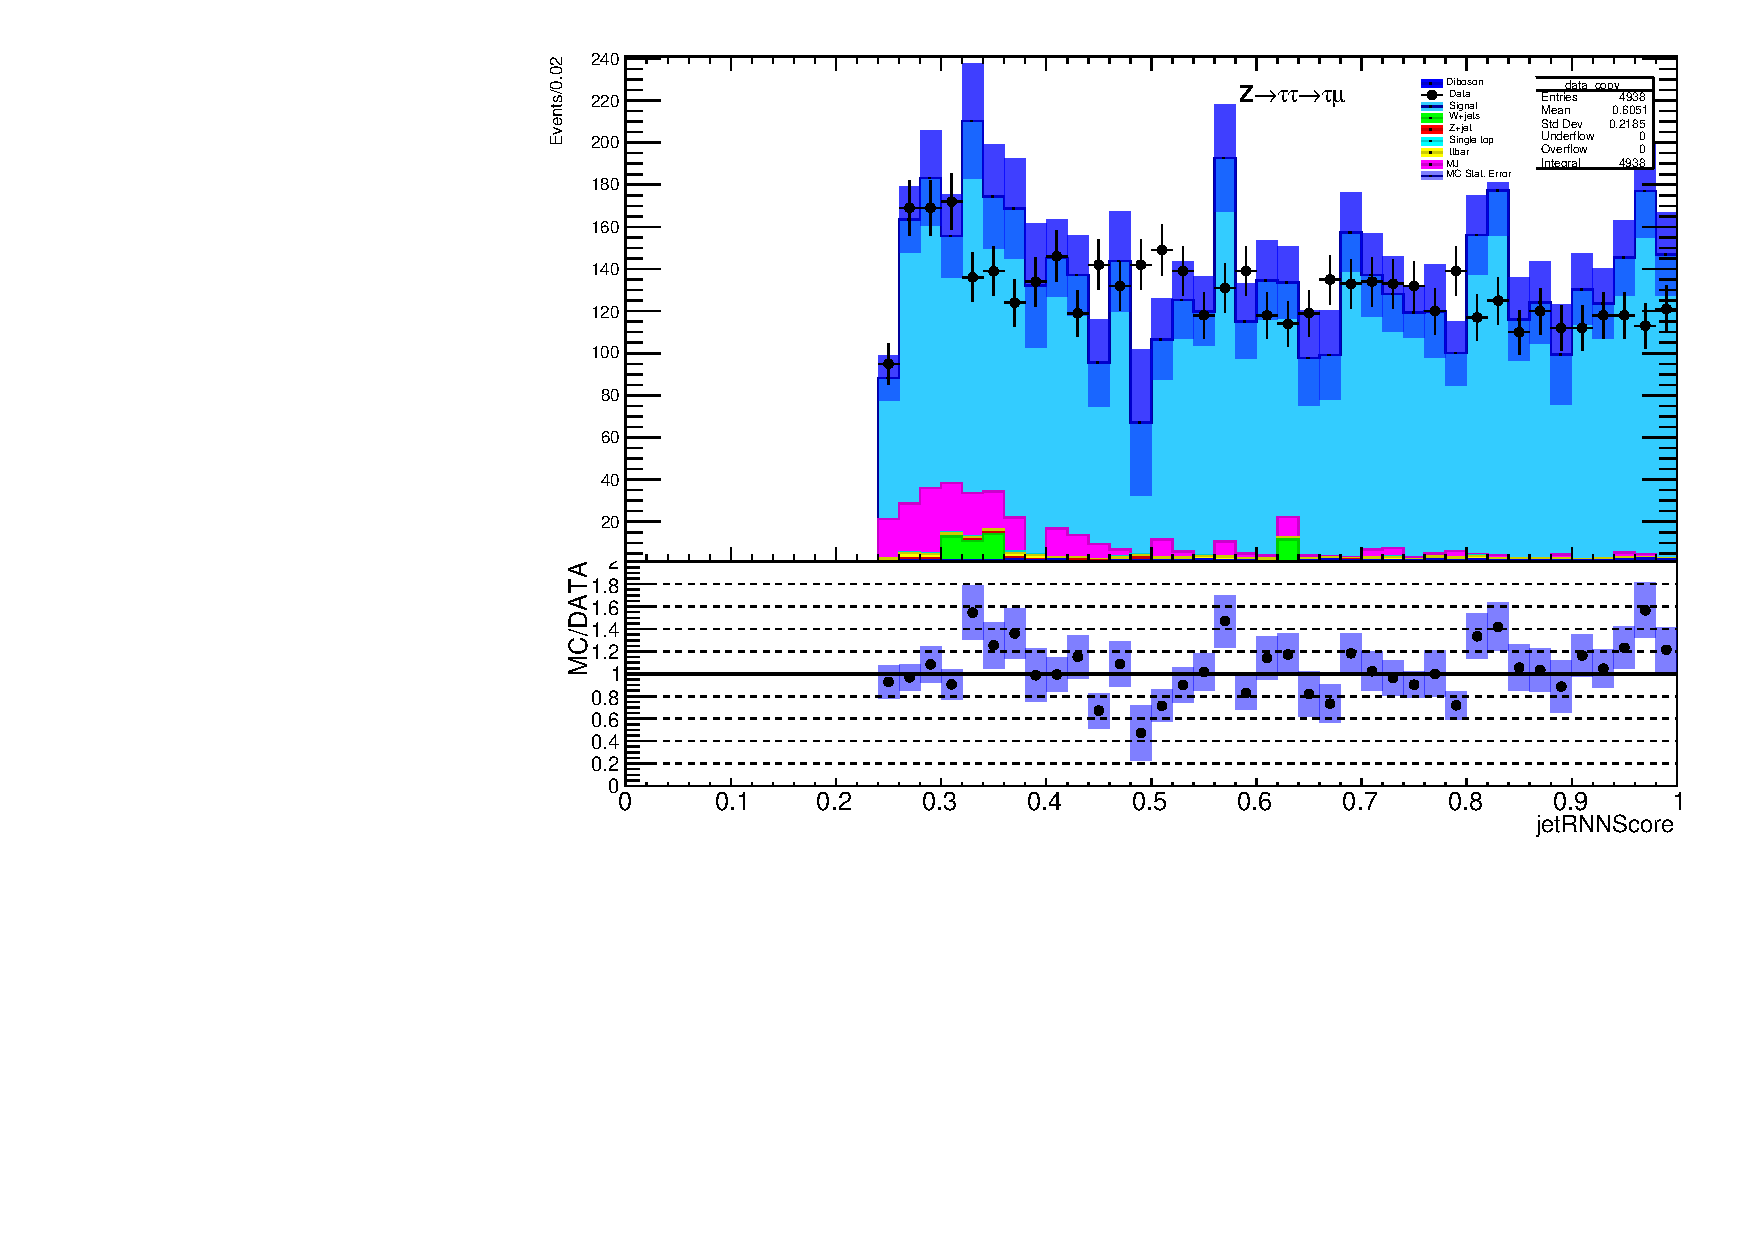
\includegraphics[width=0.50\textwidth]{figures/Fig17d}}}\hfill
	\subfloat[]{\label{Fig17e}{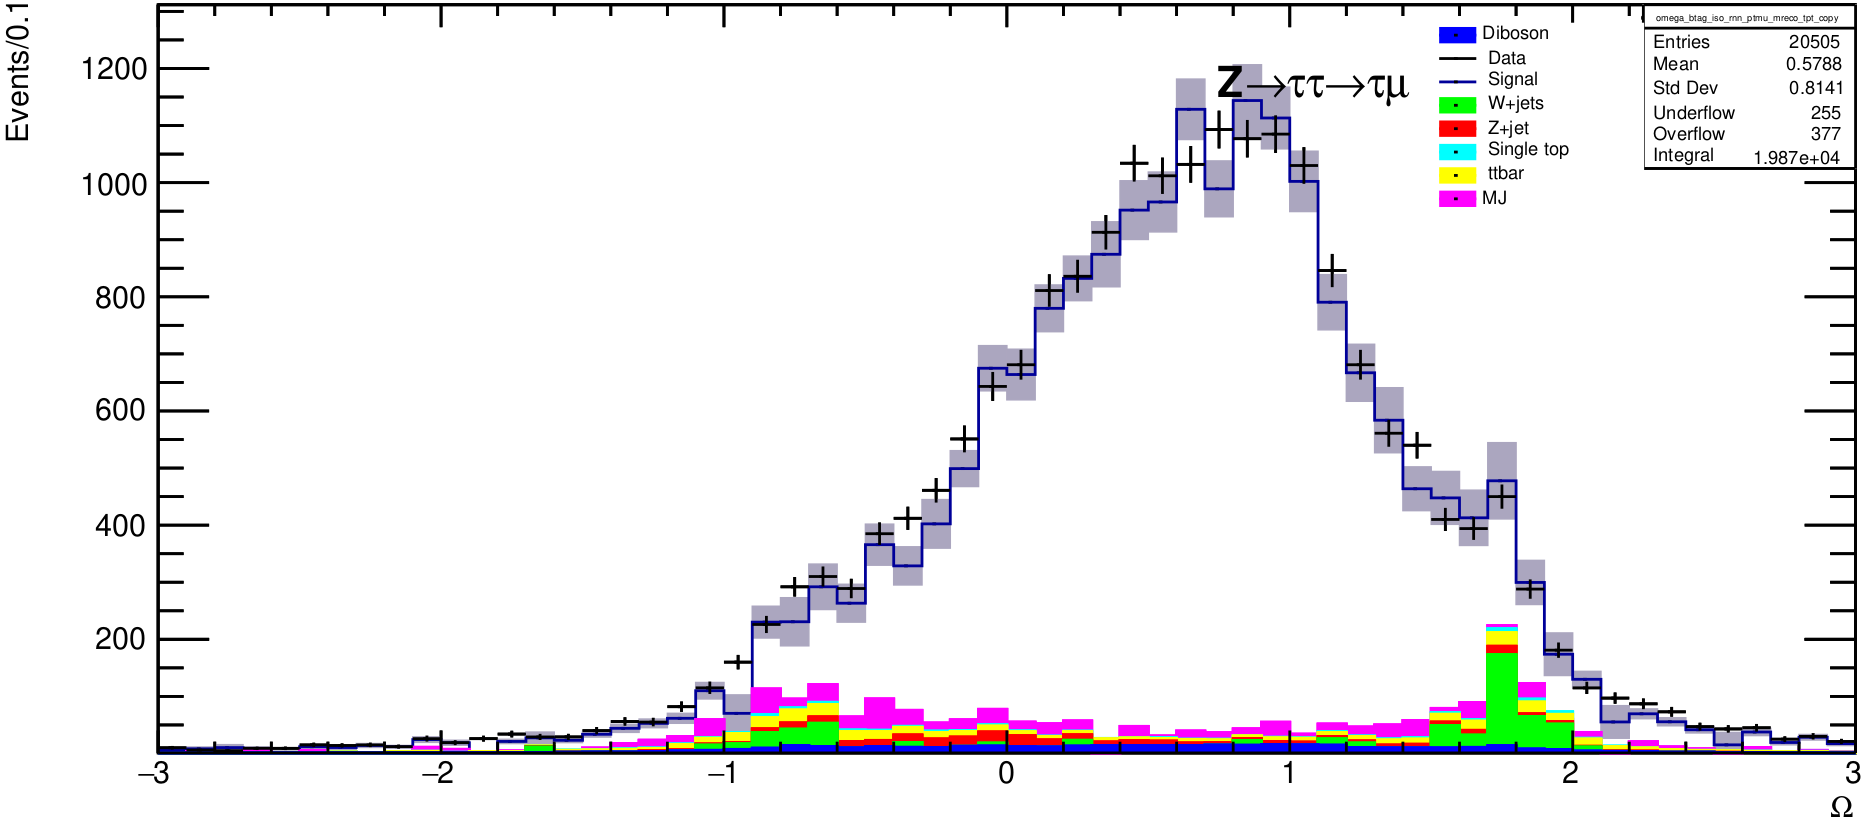
\includegraphics[width=0.50\textwidth]{figures/Fig9}}}\hfill
	\subfloat[]{\label{Fig17f}{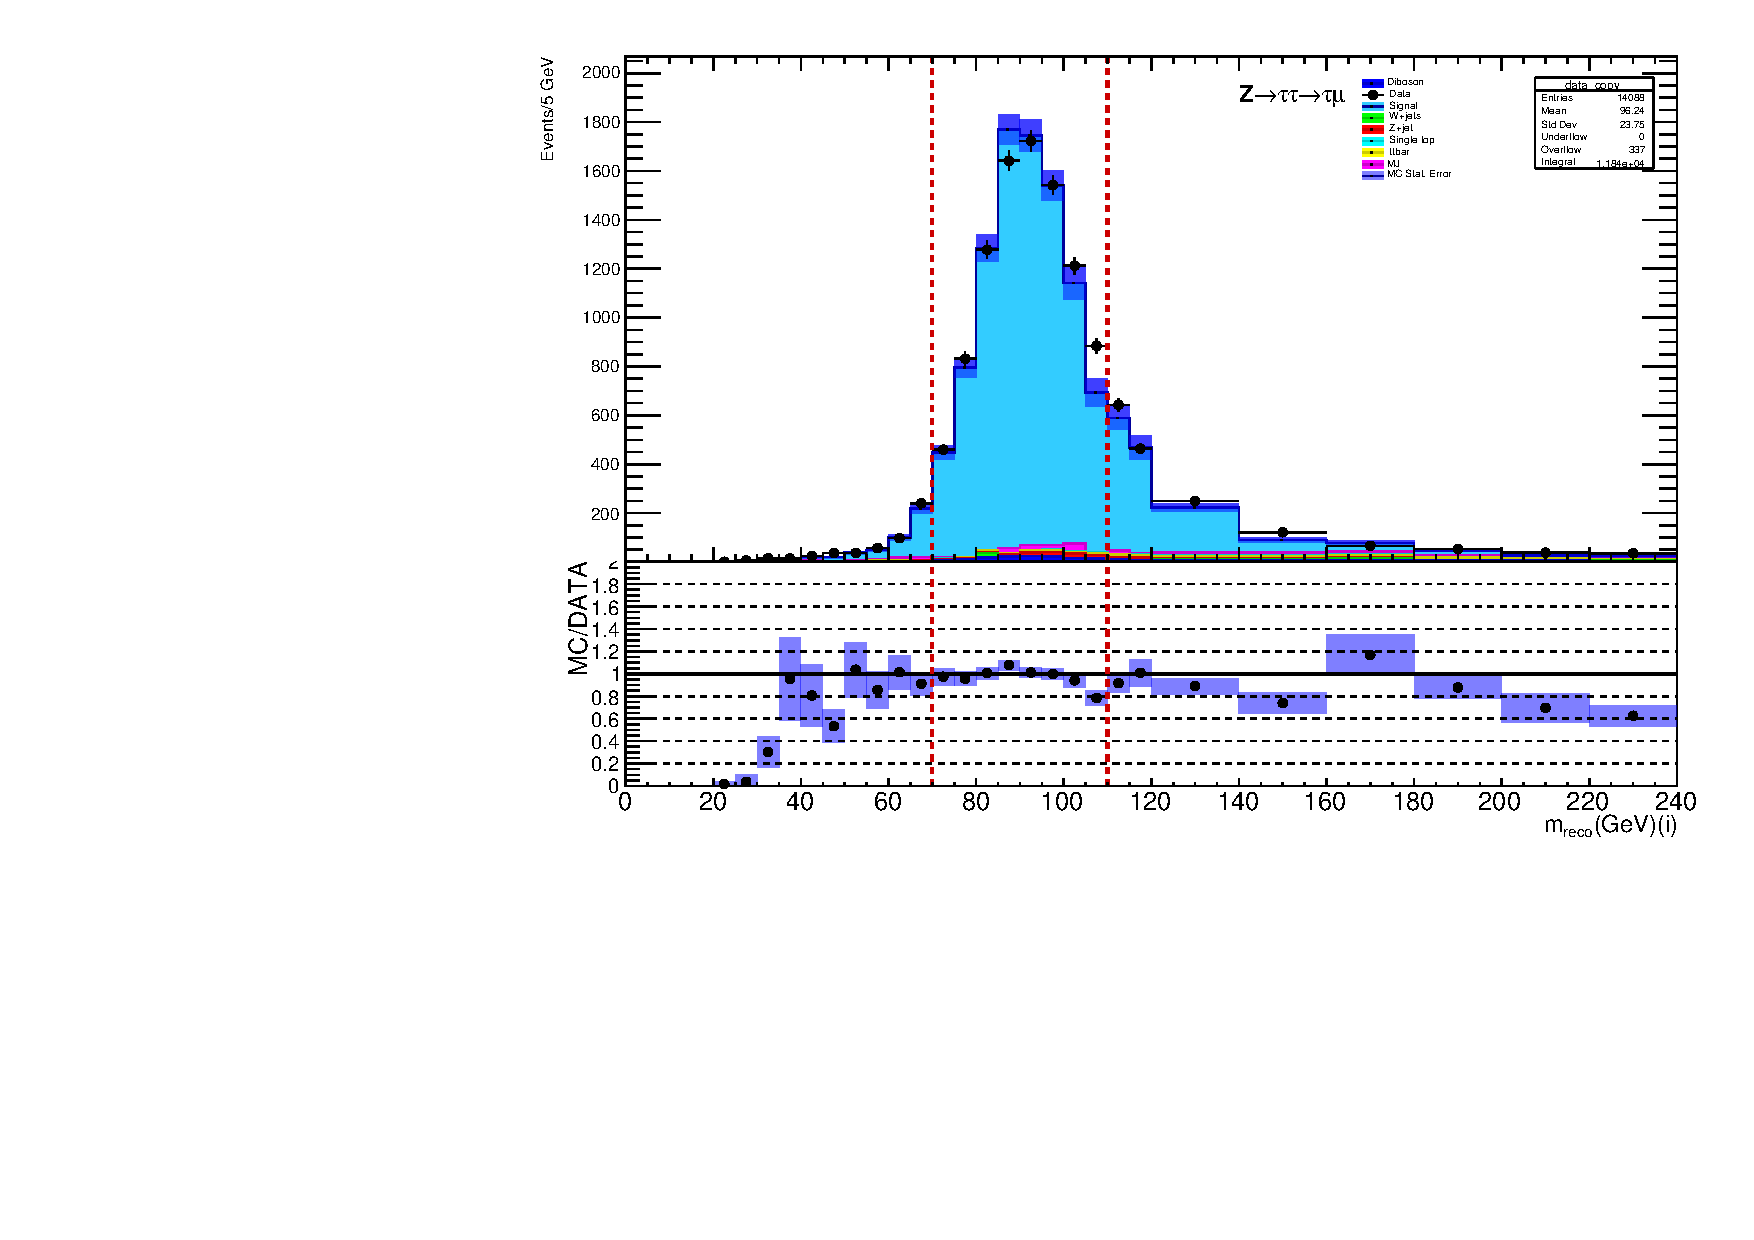
\includegraphics[width=0.50\textwidth]{figures/Fig17f}}}\hfill
	\subfloat[]{\label{Fig17g}{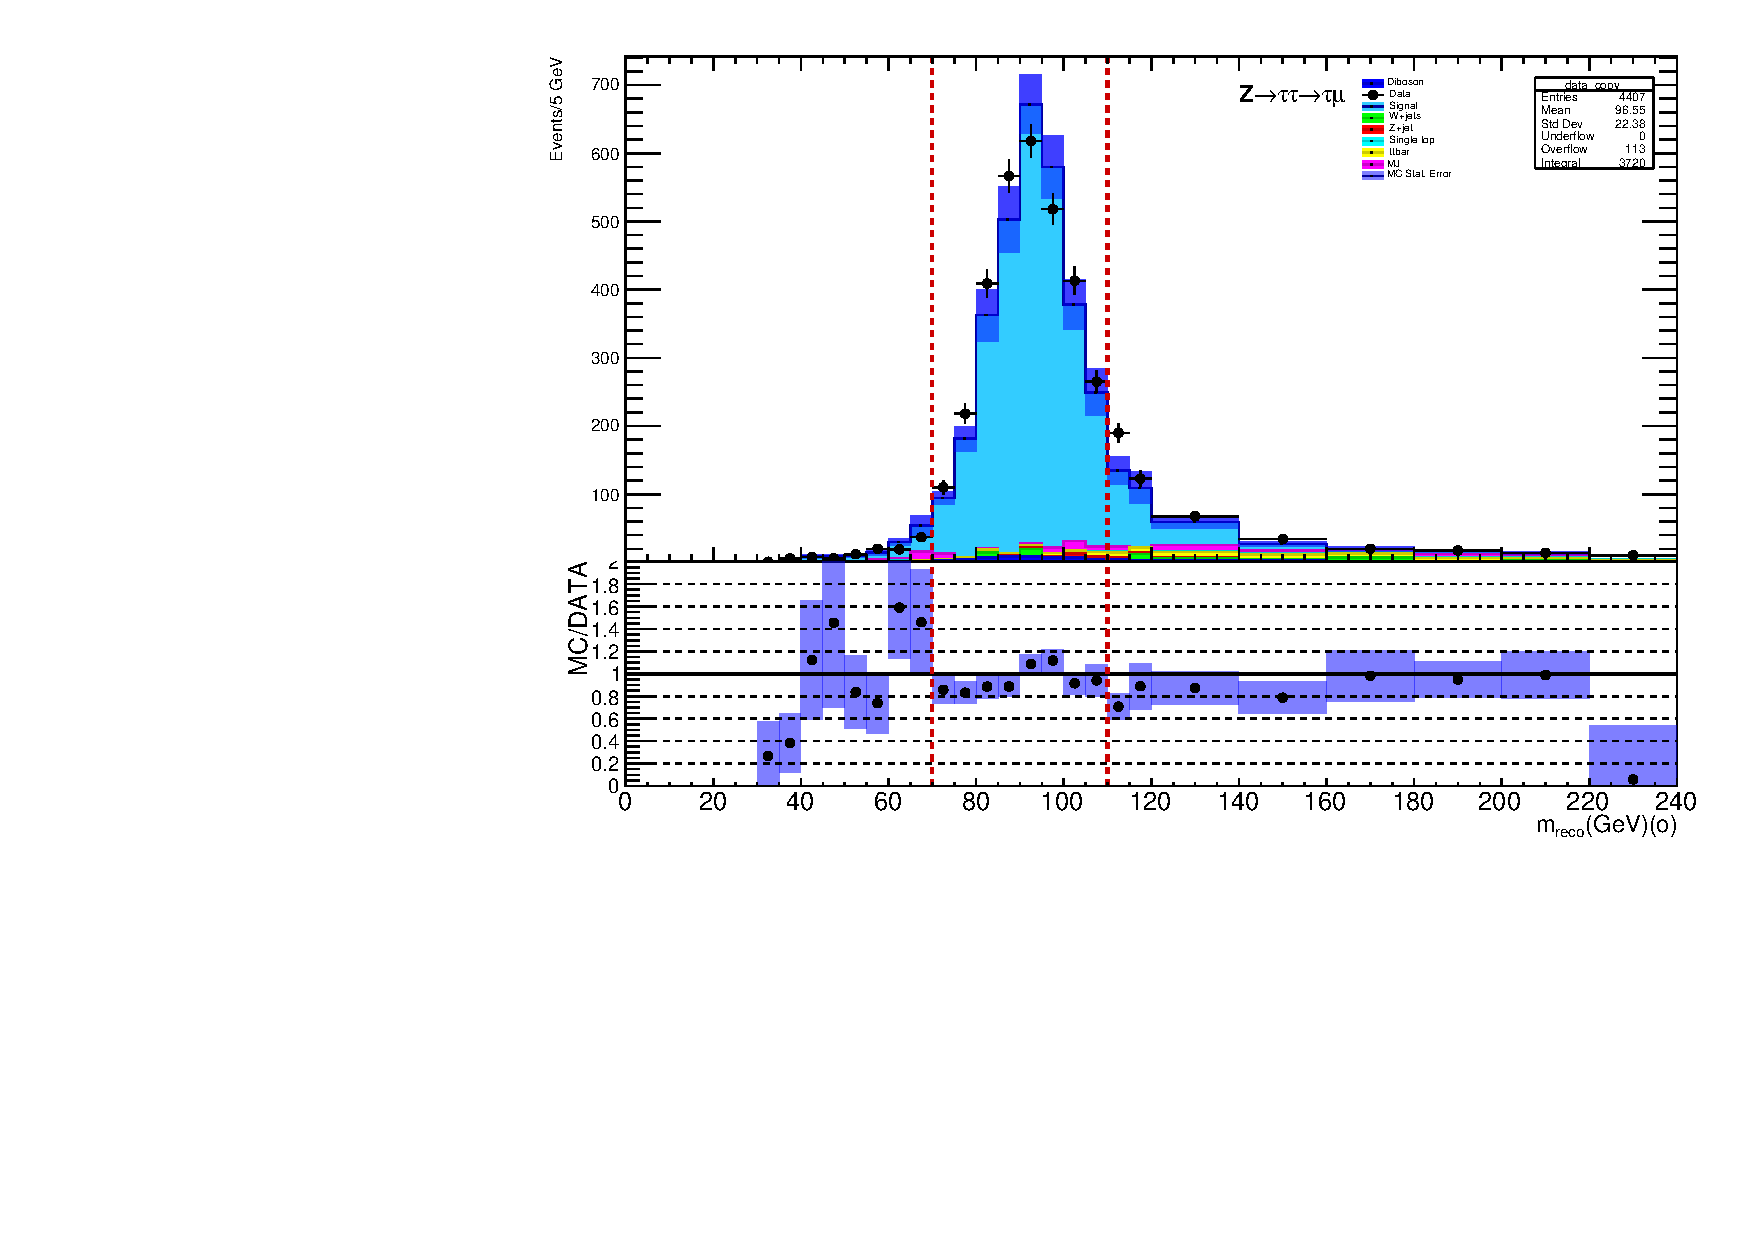
\includegraphics[width=0.50\textwidth]{figures/Fig17g}}}\hfill
	\subfloat[]{\label{Fig17h}{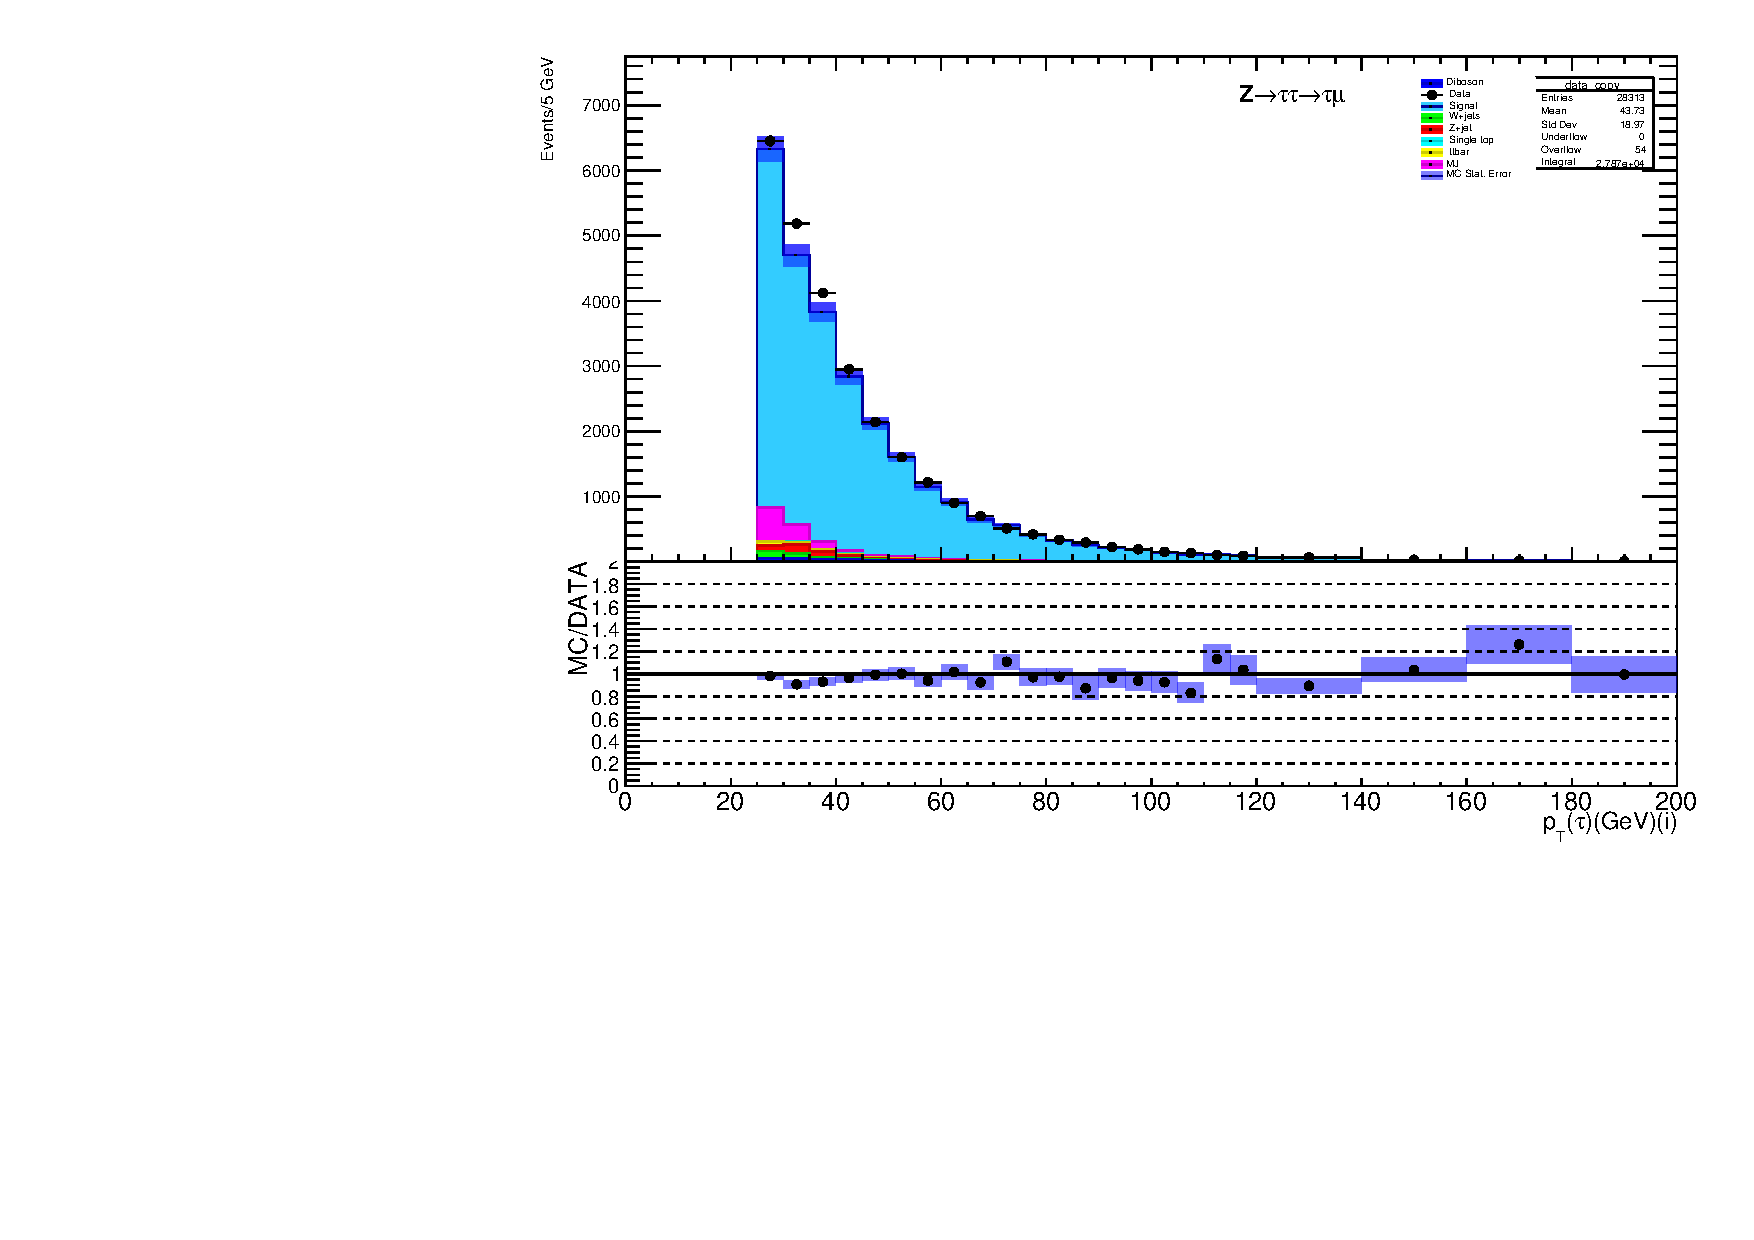
\includegraphics[width=0.50\textwidth]{figures/Fig17h}}}
	\label{Fig17}
\end{figure}
\begin{figure}[ht]\ContinuedFloat
	\centering
	\subfloat[]{\label{Fig17i}{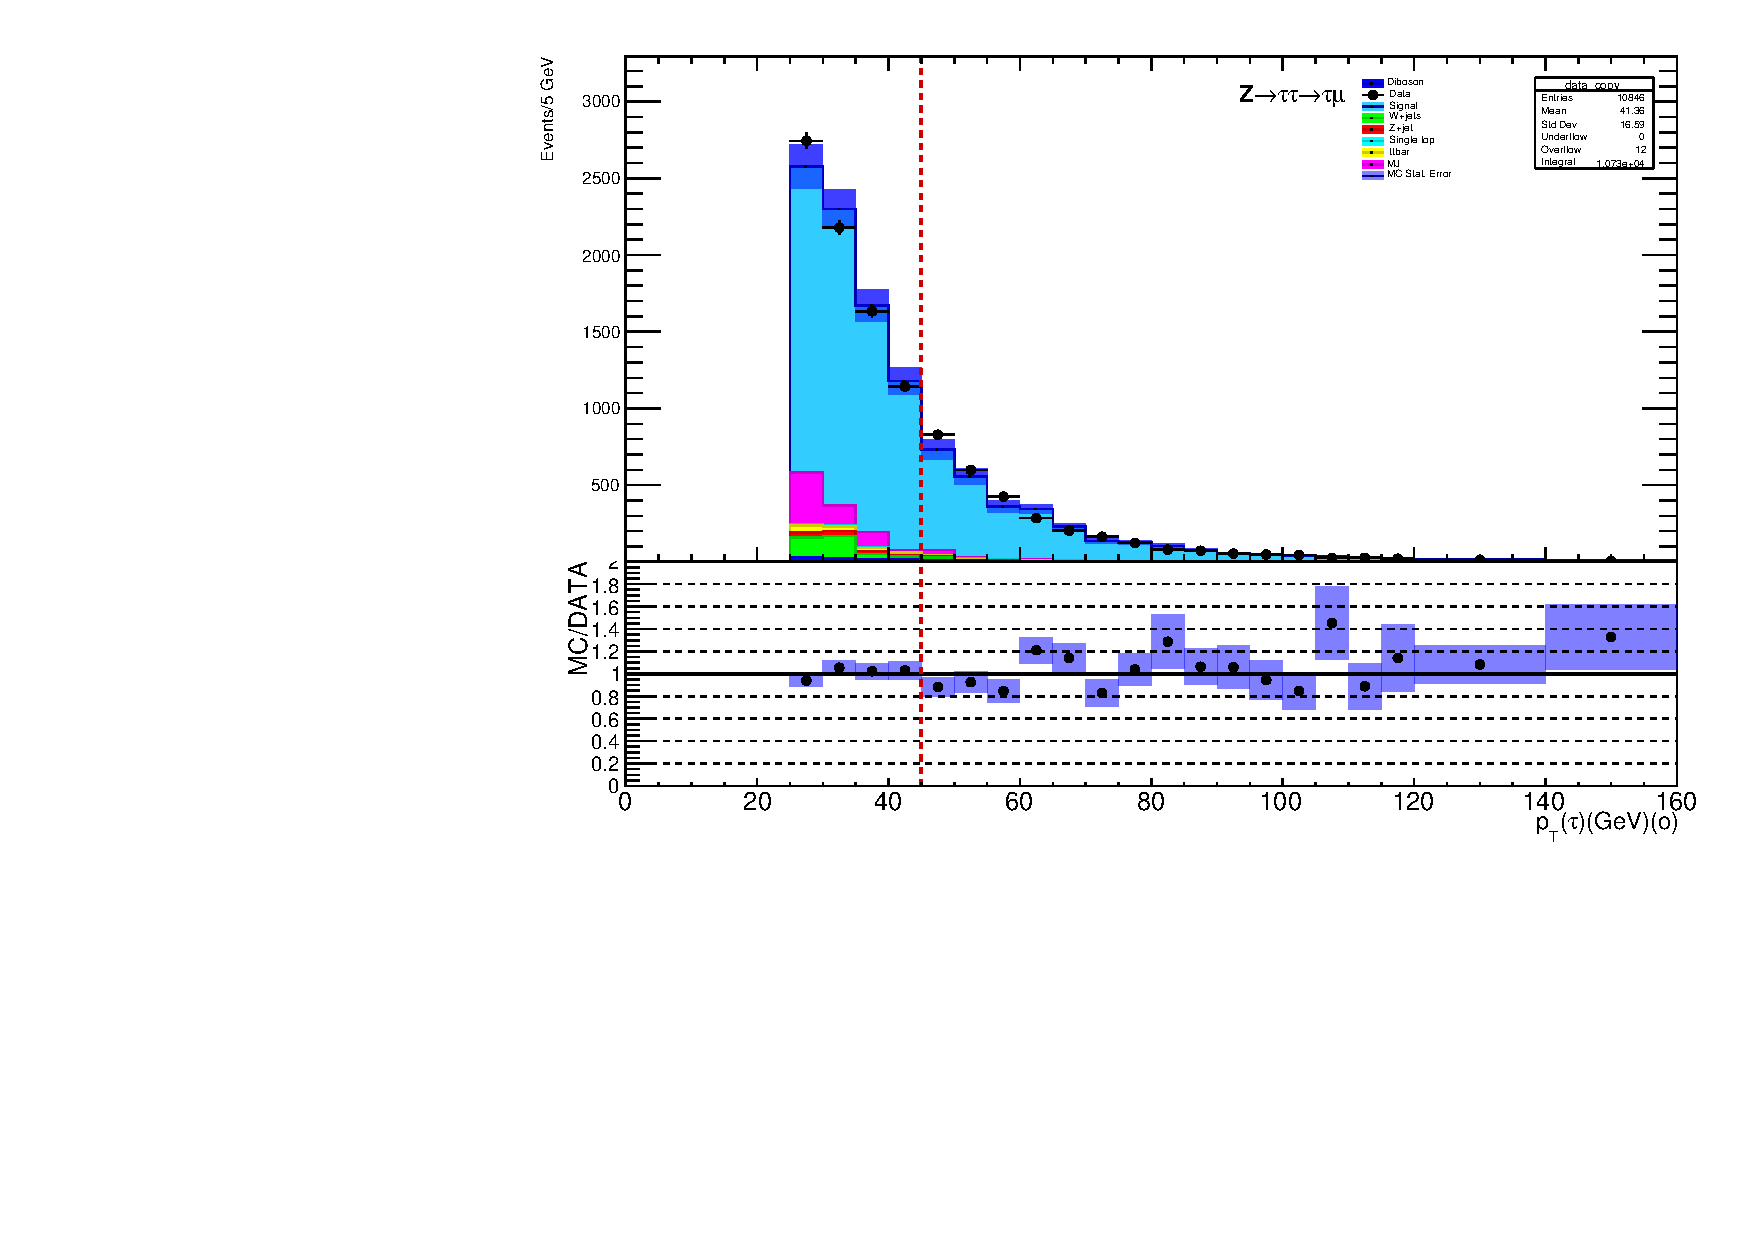
\includegraphics[width=0.50\textwidth]{figures/Fig17i}}}
	\caption{$\mreco$ distribution for the in between region (a) and the outside region (b). All the other cuts have been applied apart from the one being plotted.}
	\label{Fig17}
\end{figure}%
\newpage
\section{$Z\to\tauh e$ final state distributions}

\begin{figure}[ht]
	\centering
	\subfloat[]{\label{Fig18a}{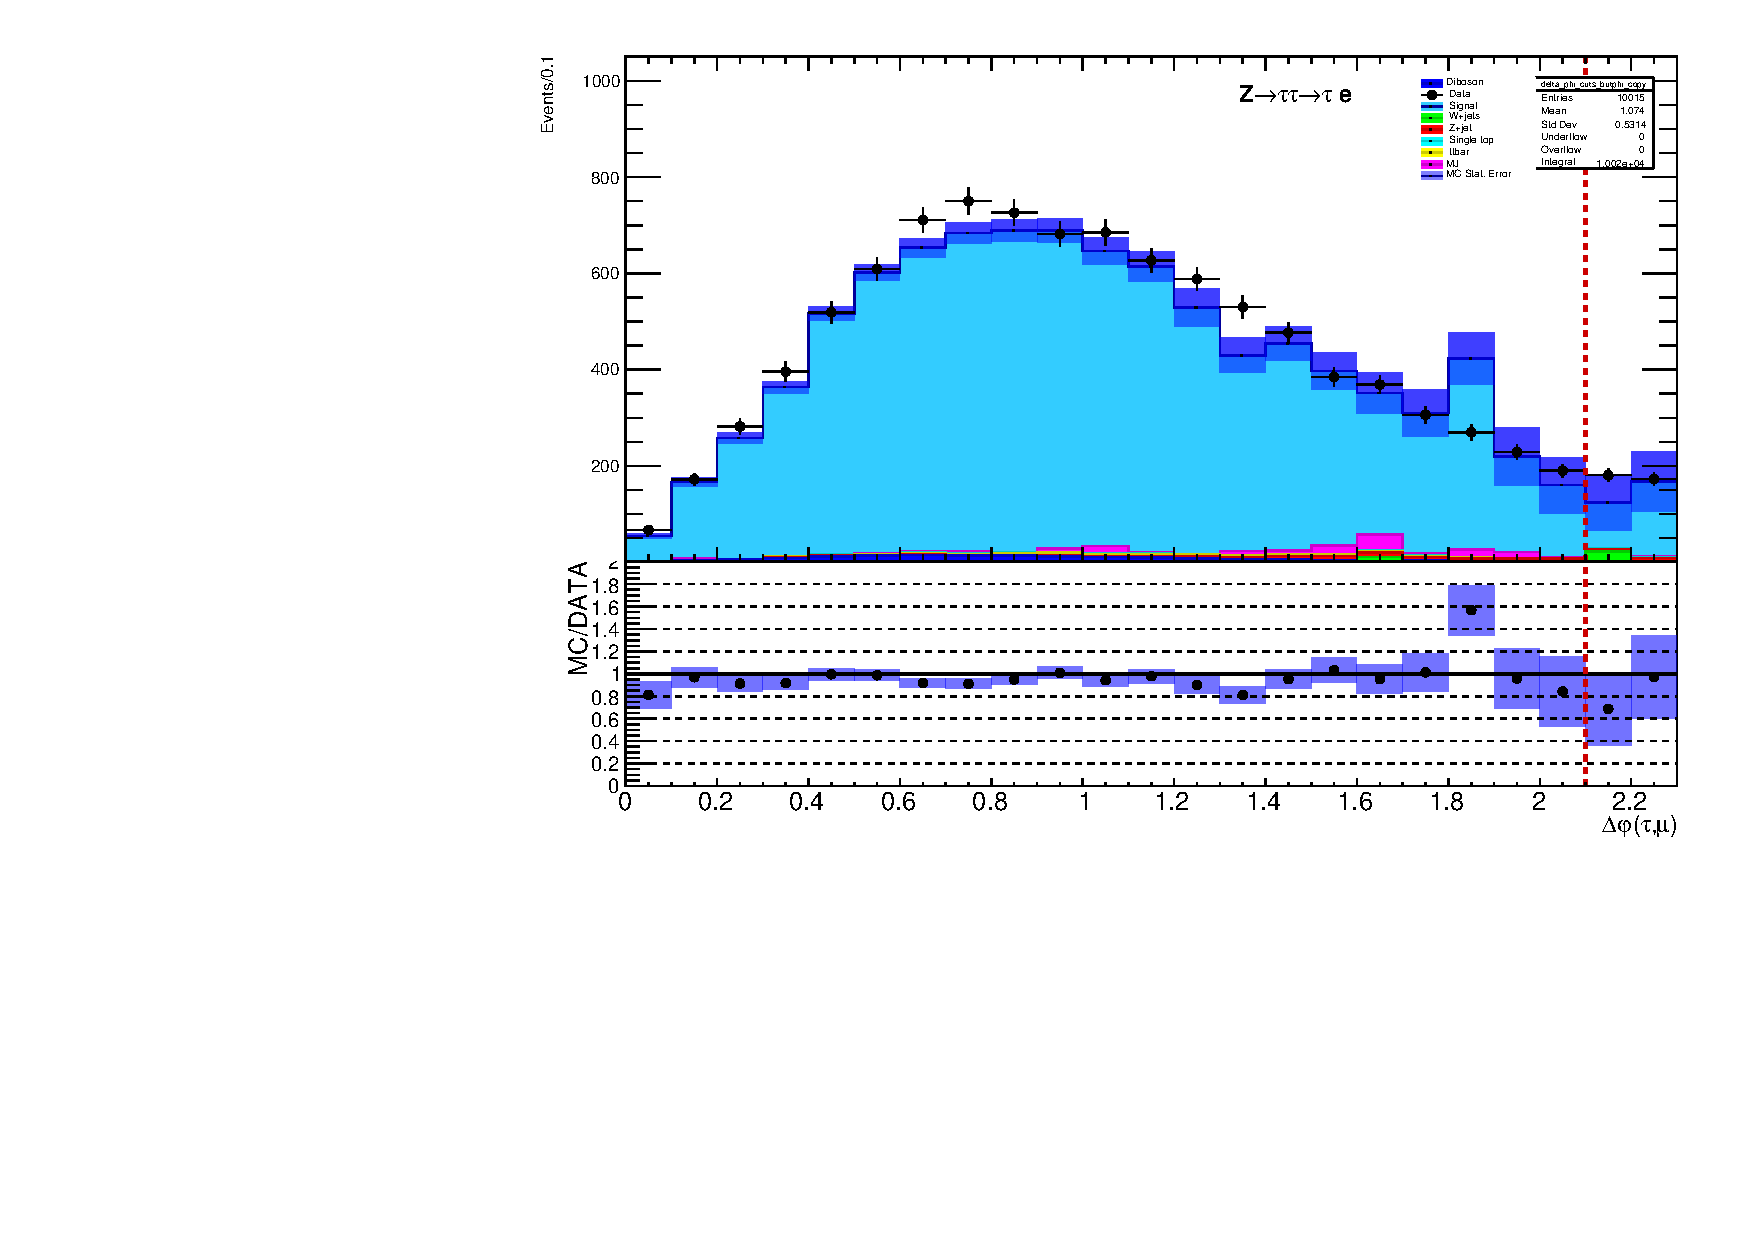
\includegraphics[width=0.50\textwidth]{figures/Fig18a}}}\hfill
	\subfloat[]{\label{Fig18b}{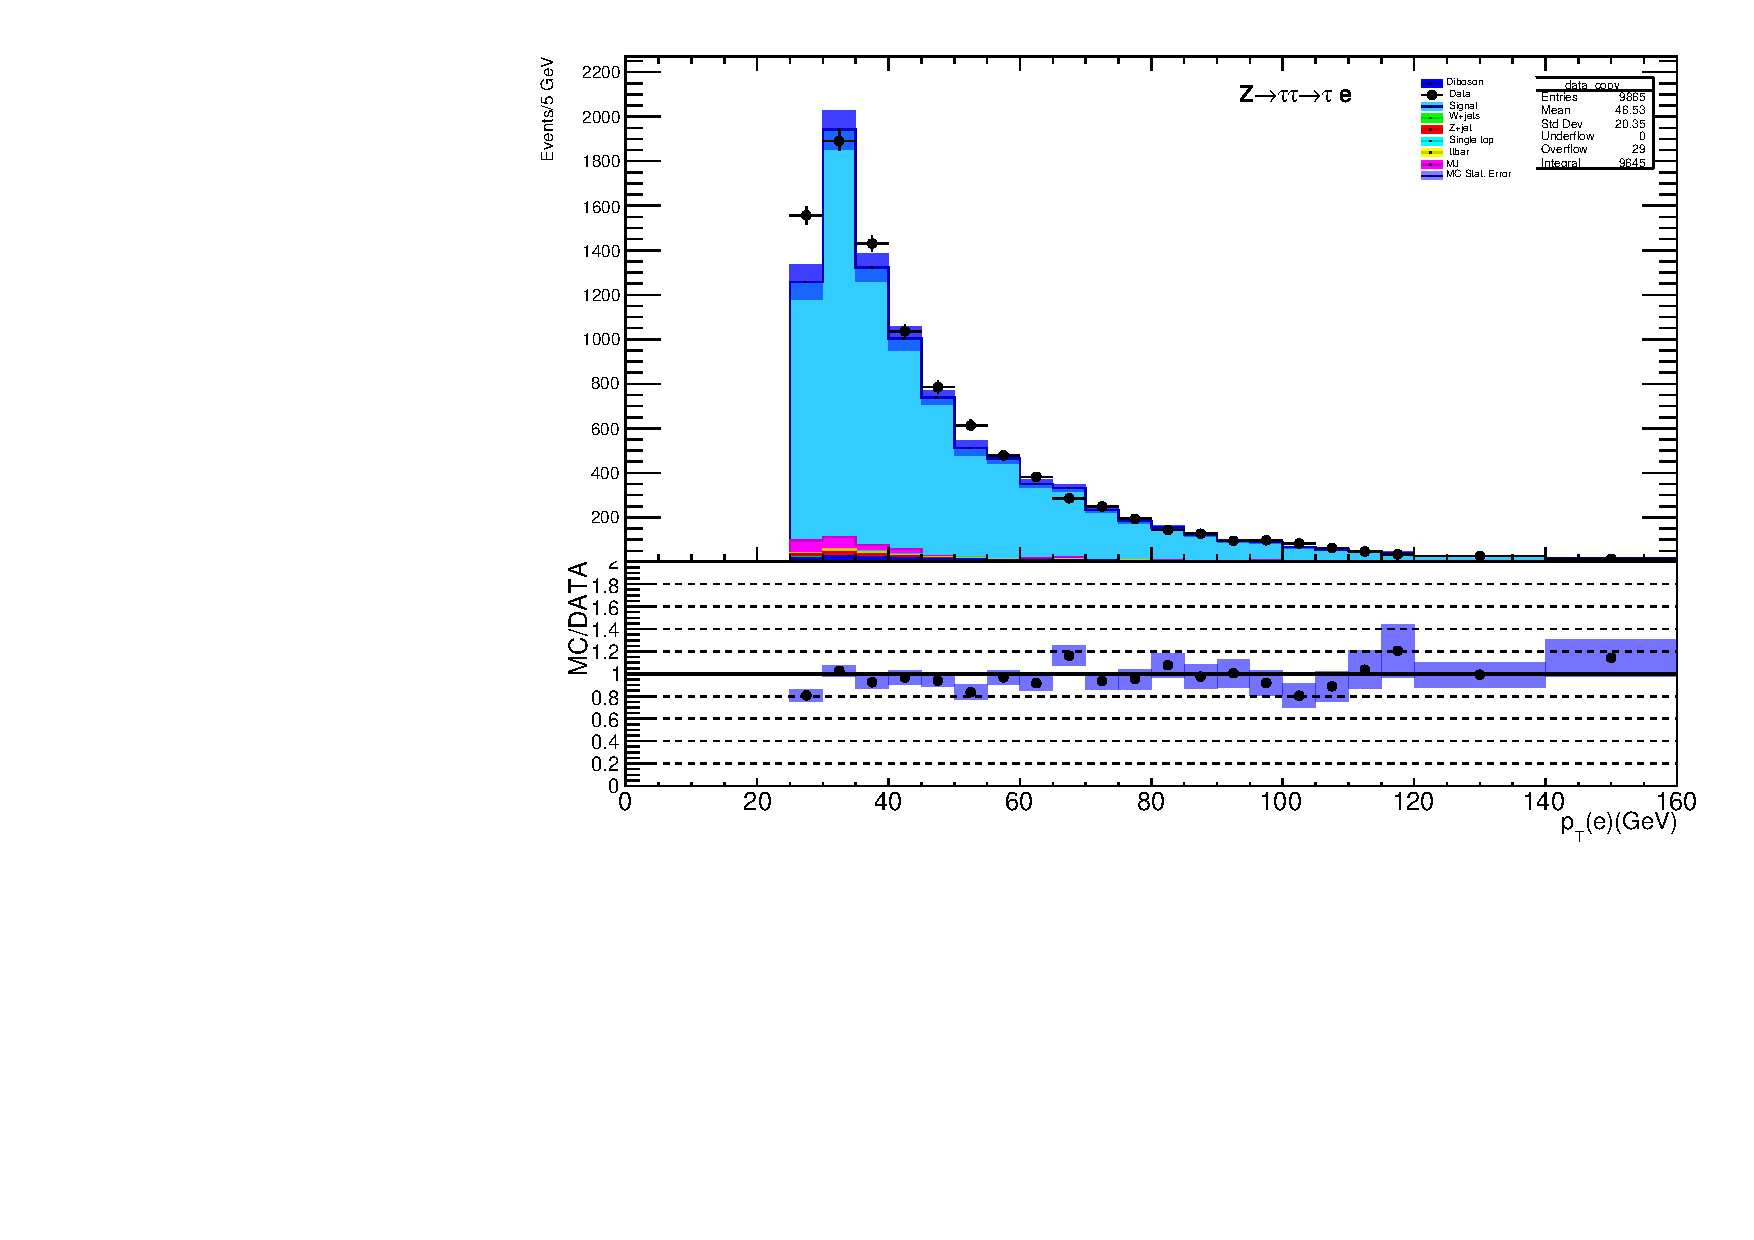
\includegraphics[width=0.50\textwidth]{figures/Fig18b}}}\hfill
	\subfloat[]{\label{Fig18c}{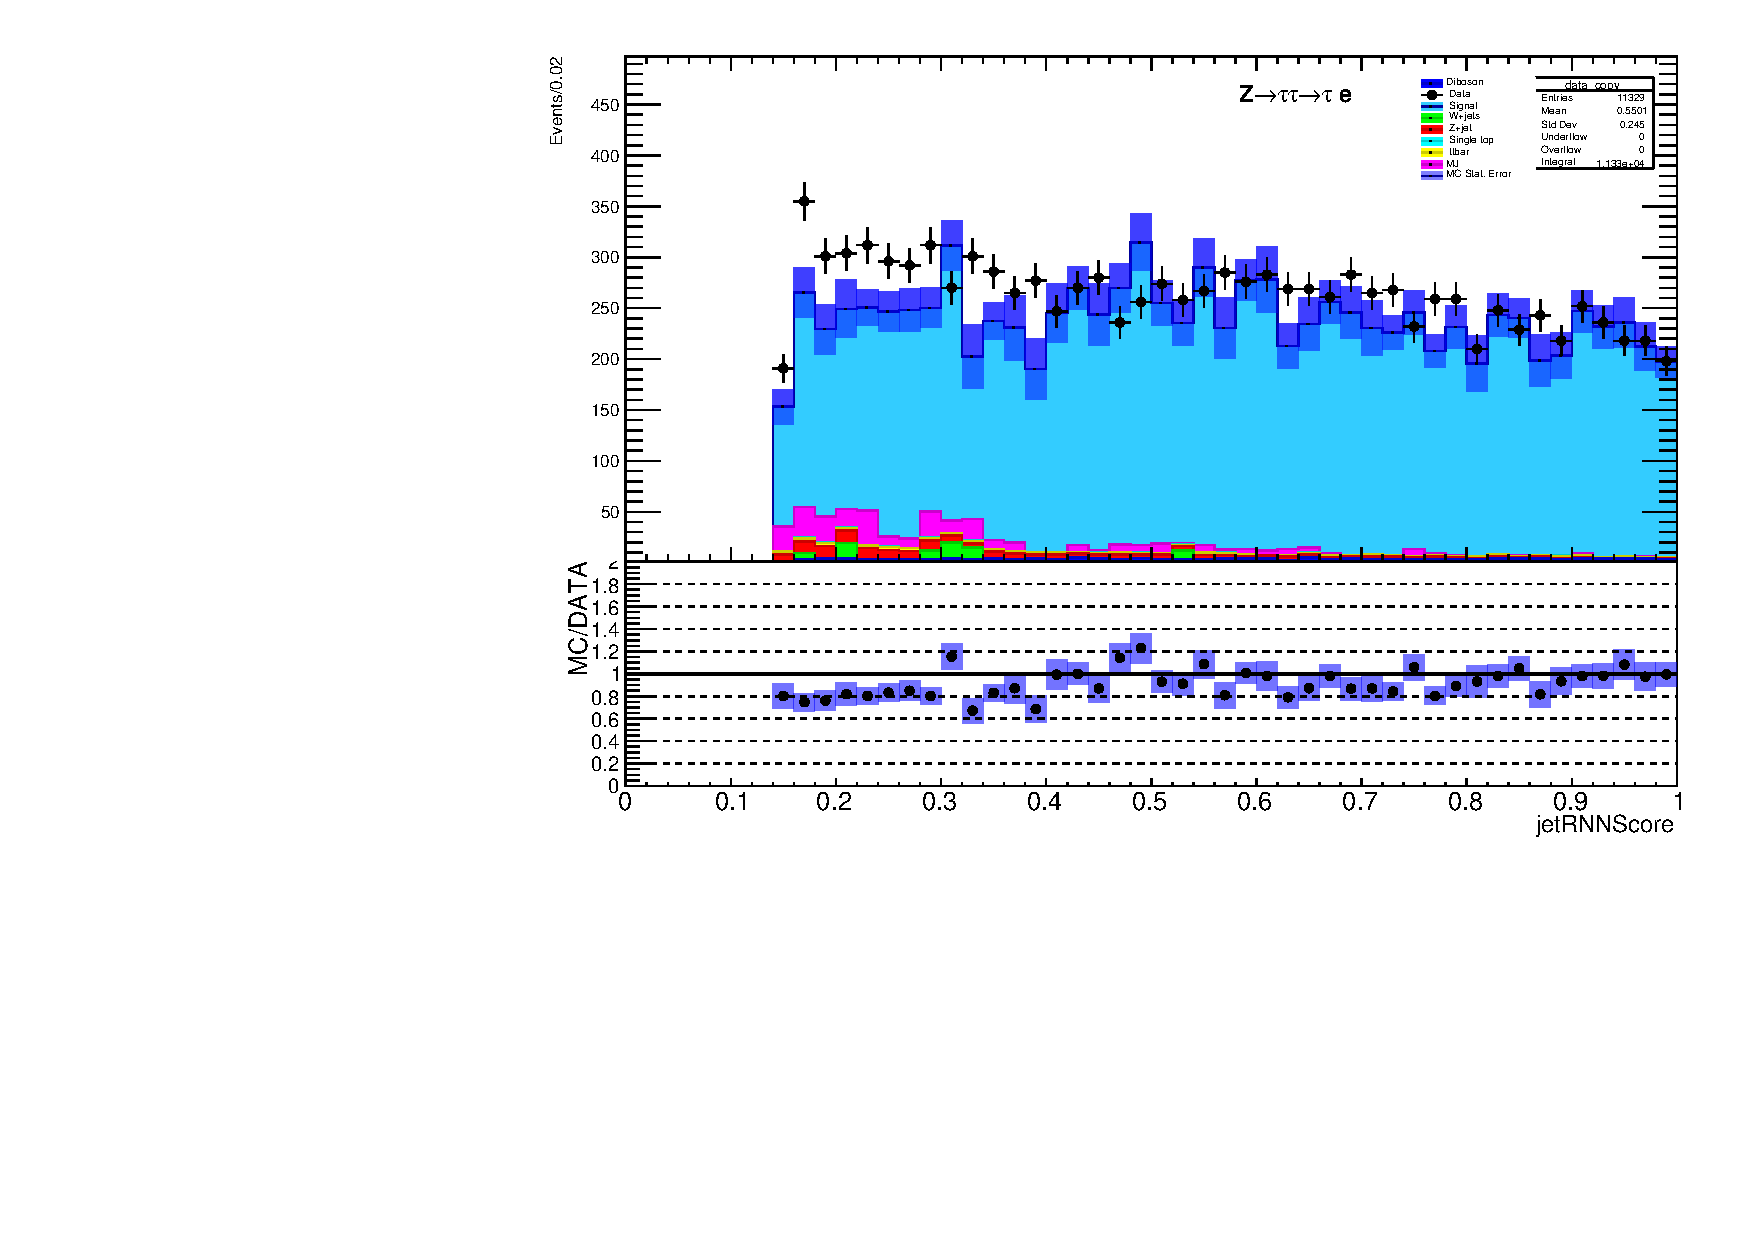
\includegraphics[width=0.50\textwidth]{figures/Fig18c}}}\hfill
	\subfloat[]{\label{Fig18d}{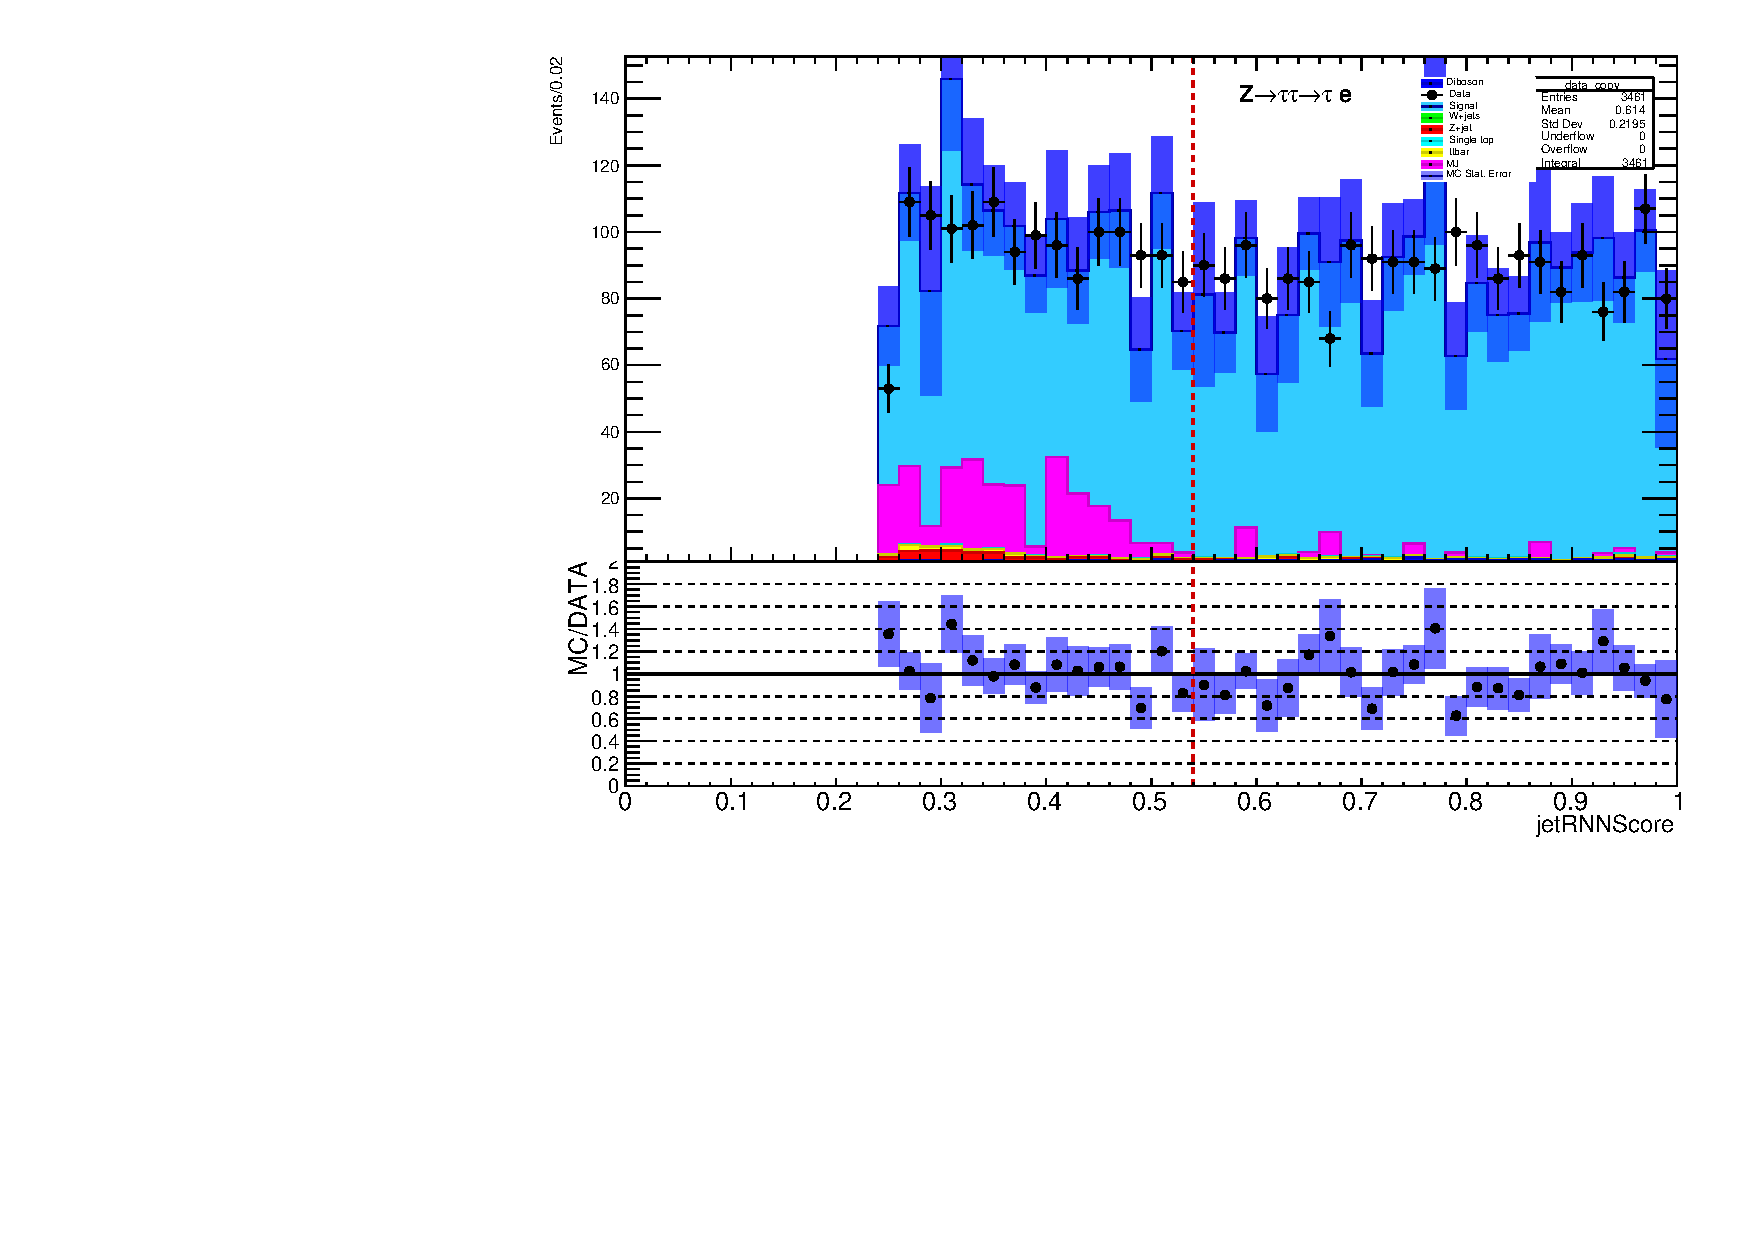
\includegraphics[width=0.50\textwidth]{figures/Fig18d}}}\hfill
	\subfloat[]{\label{Fig18e}{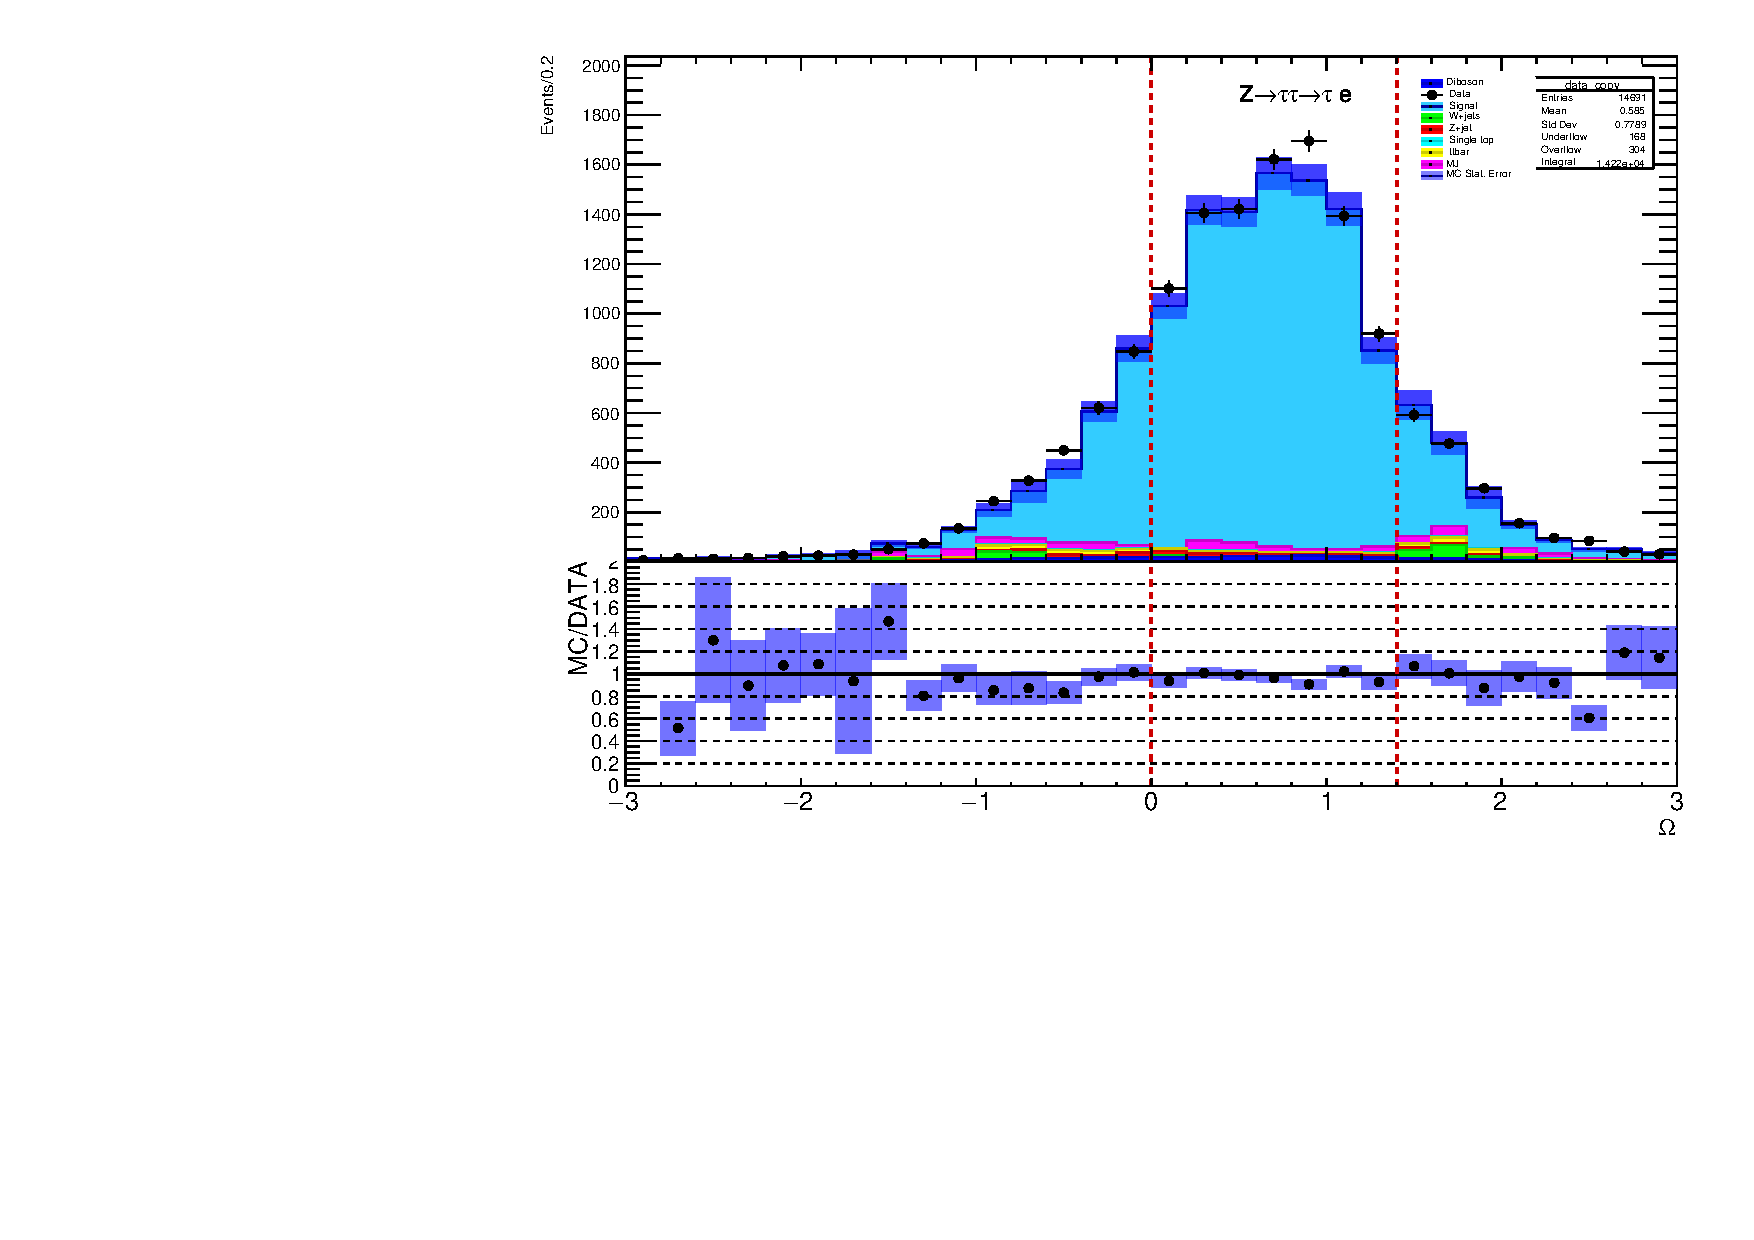
\includegraphics[width=0.50\textwidth]{figures/Fig18e}}}\hfill
	\subfloat[]{\label{Fig18f}{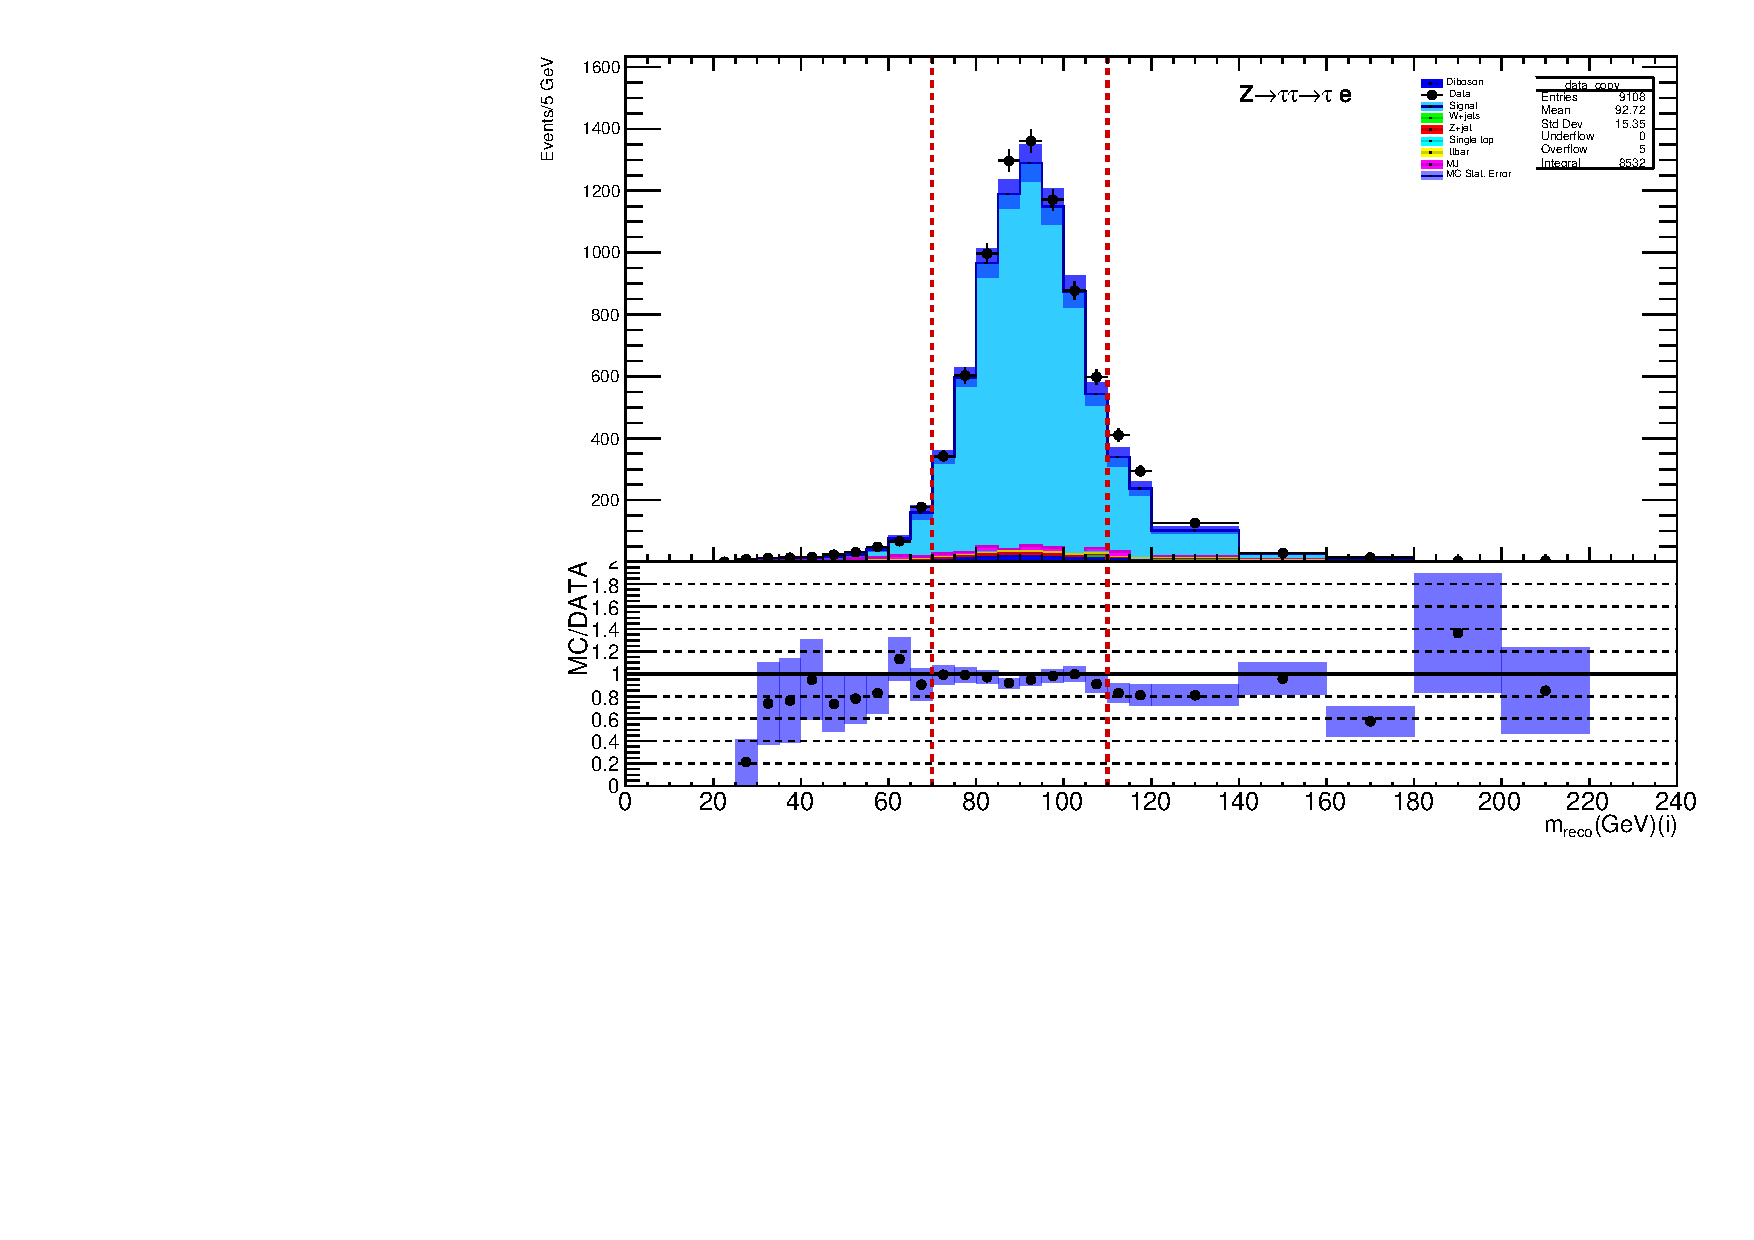
\includegraphics[width=0.50\textwidth]{figures/Fig18f}}}\hfill
	\subfloat[]{\label{Fig18g}{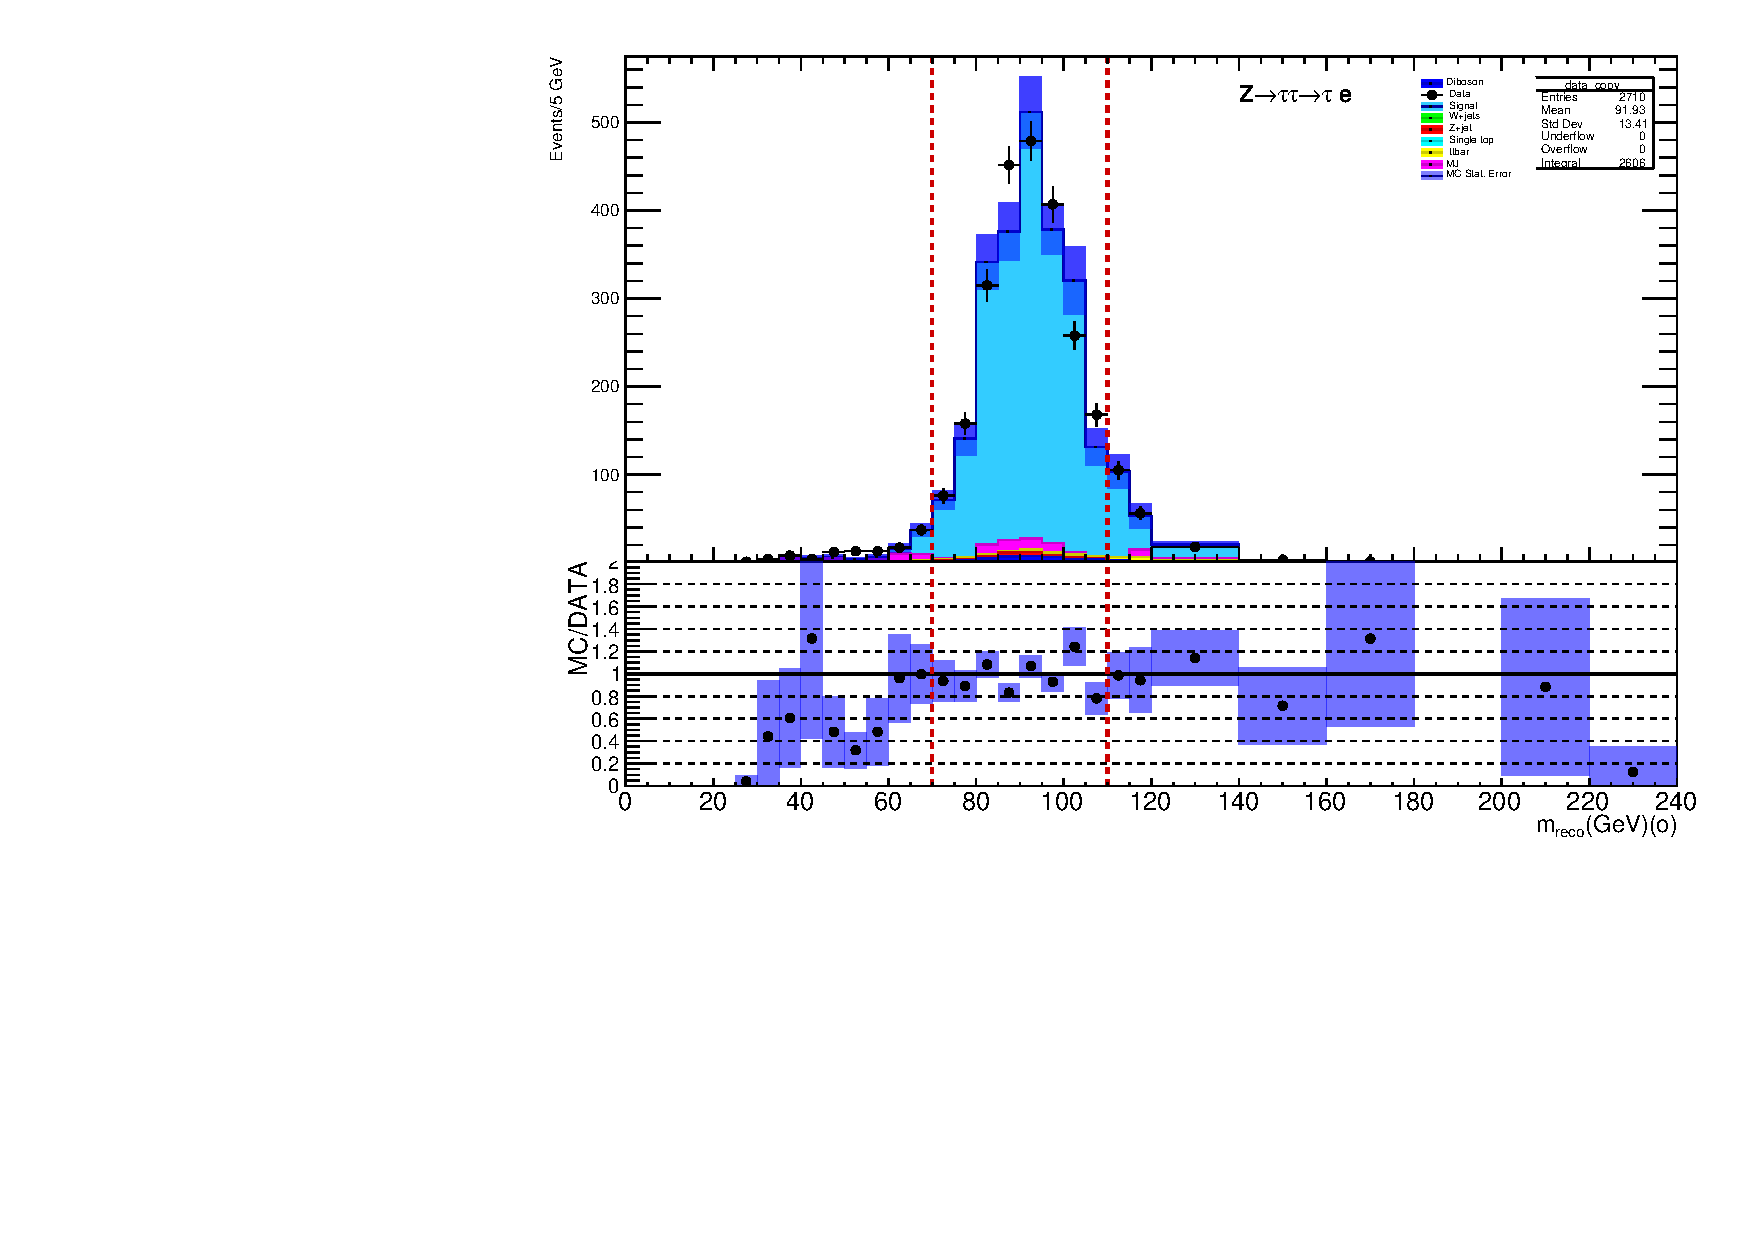
\includegraphics[width=0.50\textwidth]{figures/Fig18g}}}\hfill
	\subfloat[]{\label{Fig18h}{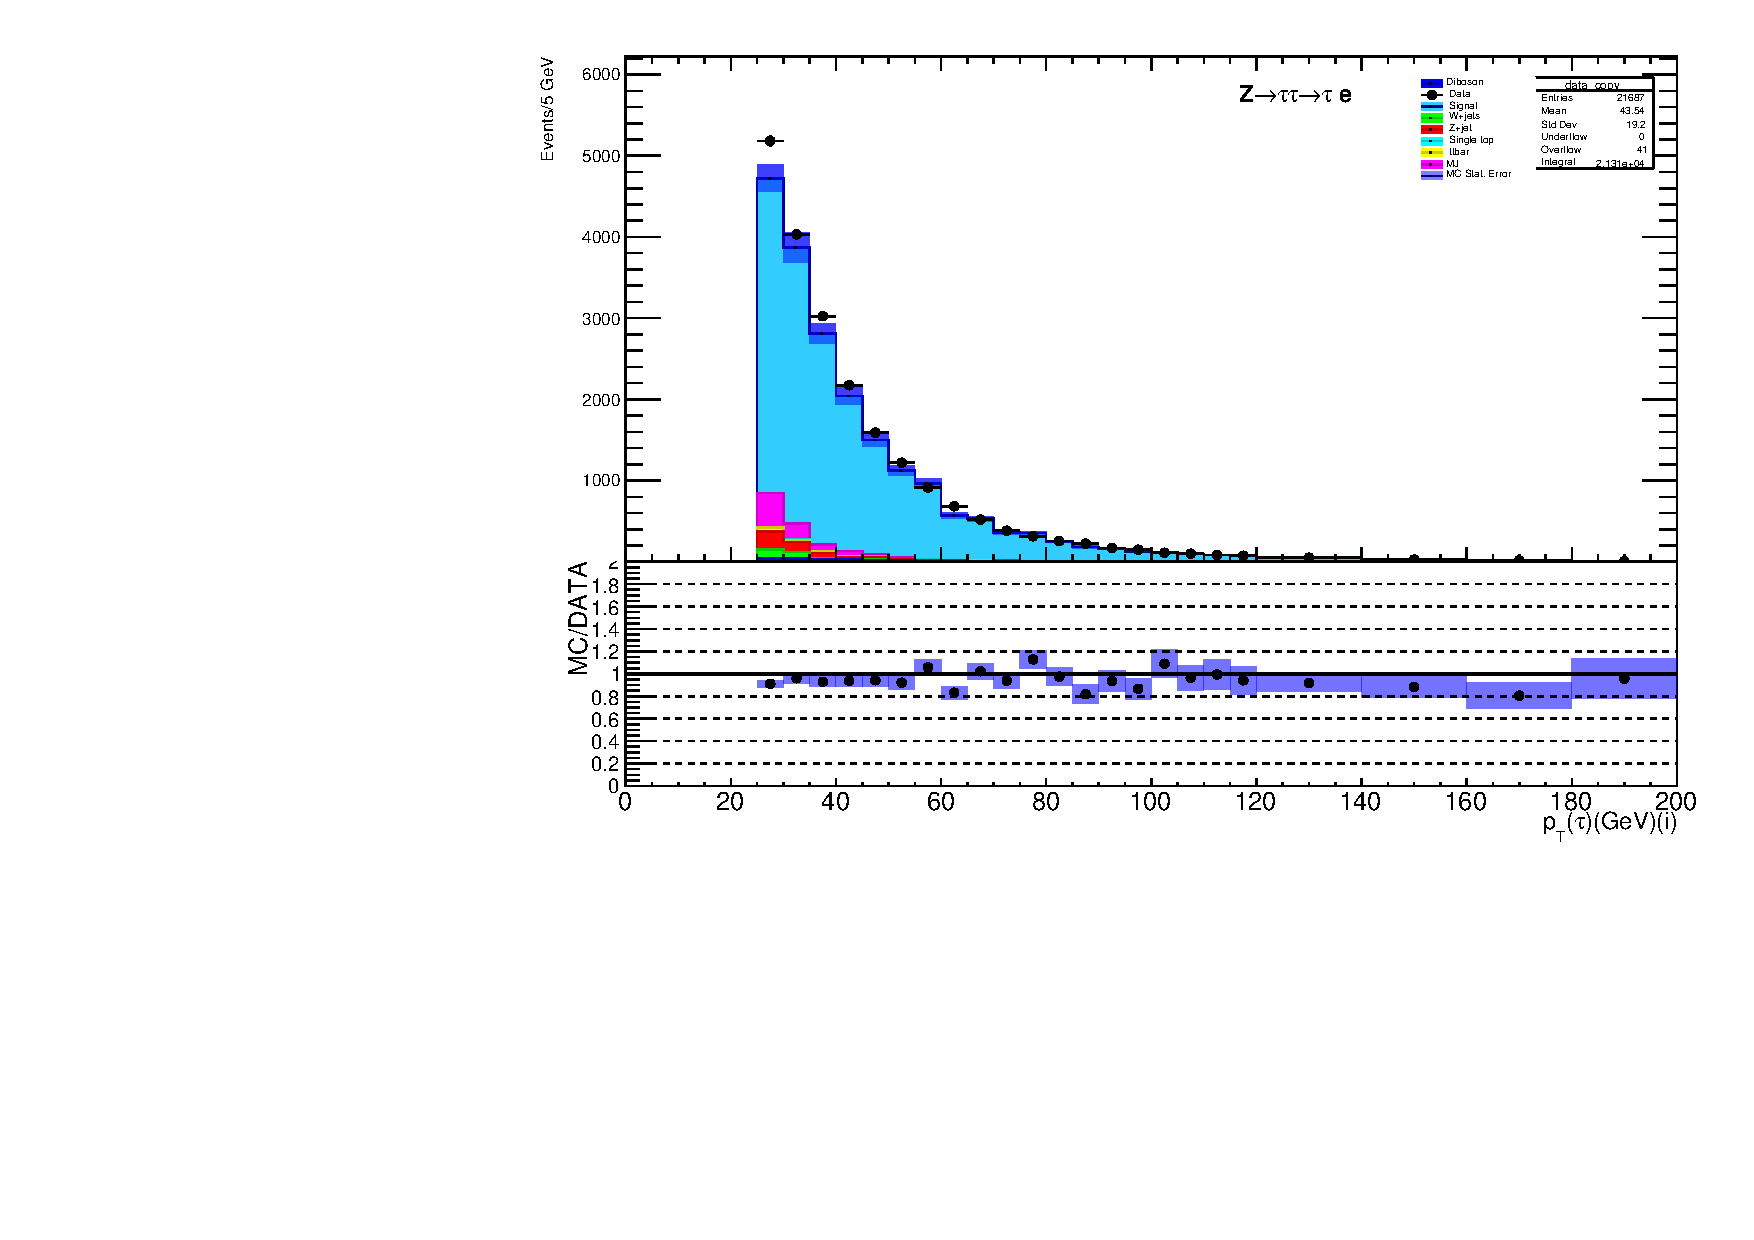
\includegraphics[width=0.50\textwidth]{figures/Fig18h}}}
	\label{Fig18}
\end{figure}
\begin{figure}[ht]\ContinuedFloat
	\centering
	\subfloat[]{\label{Fig18i}{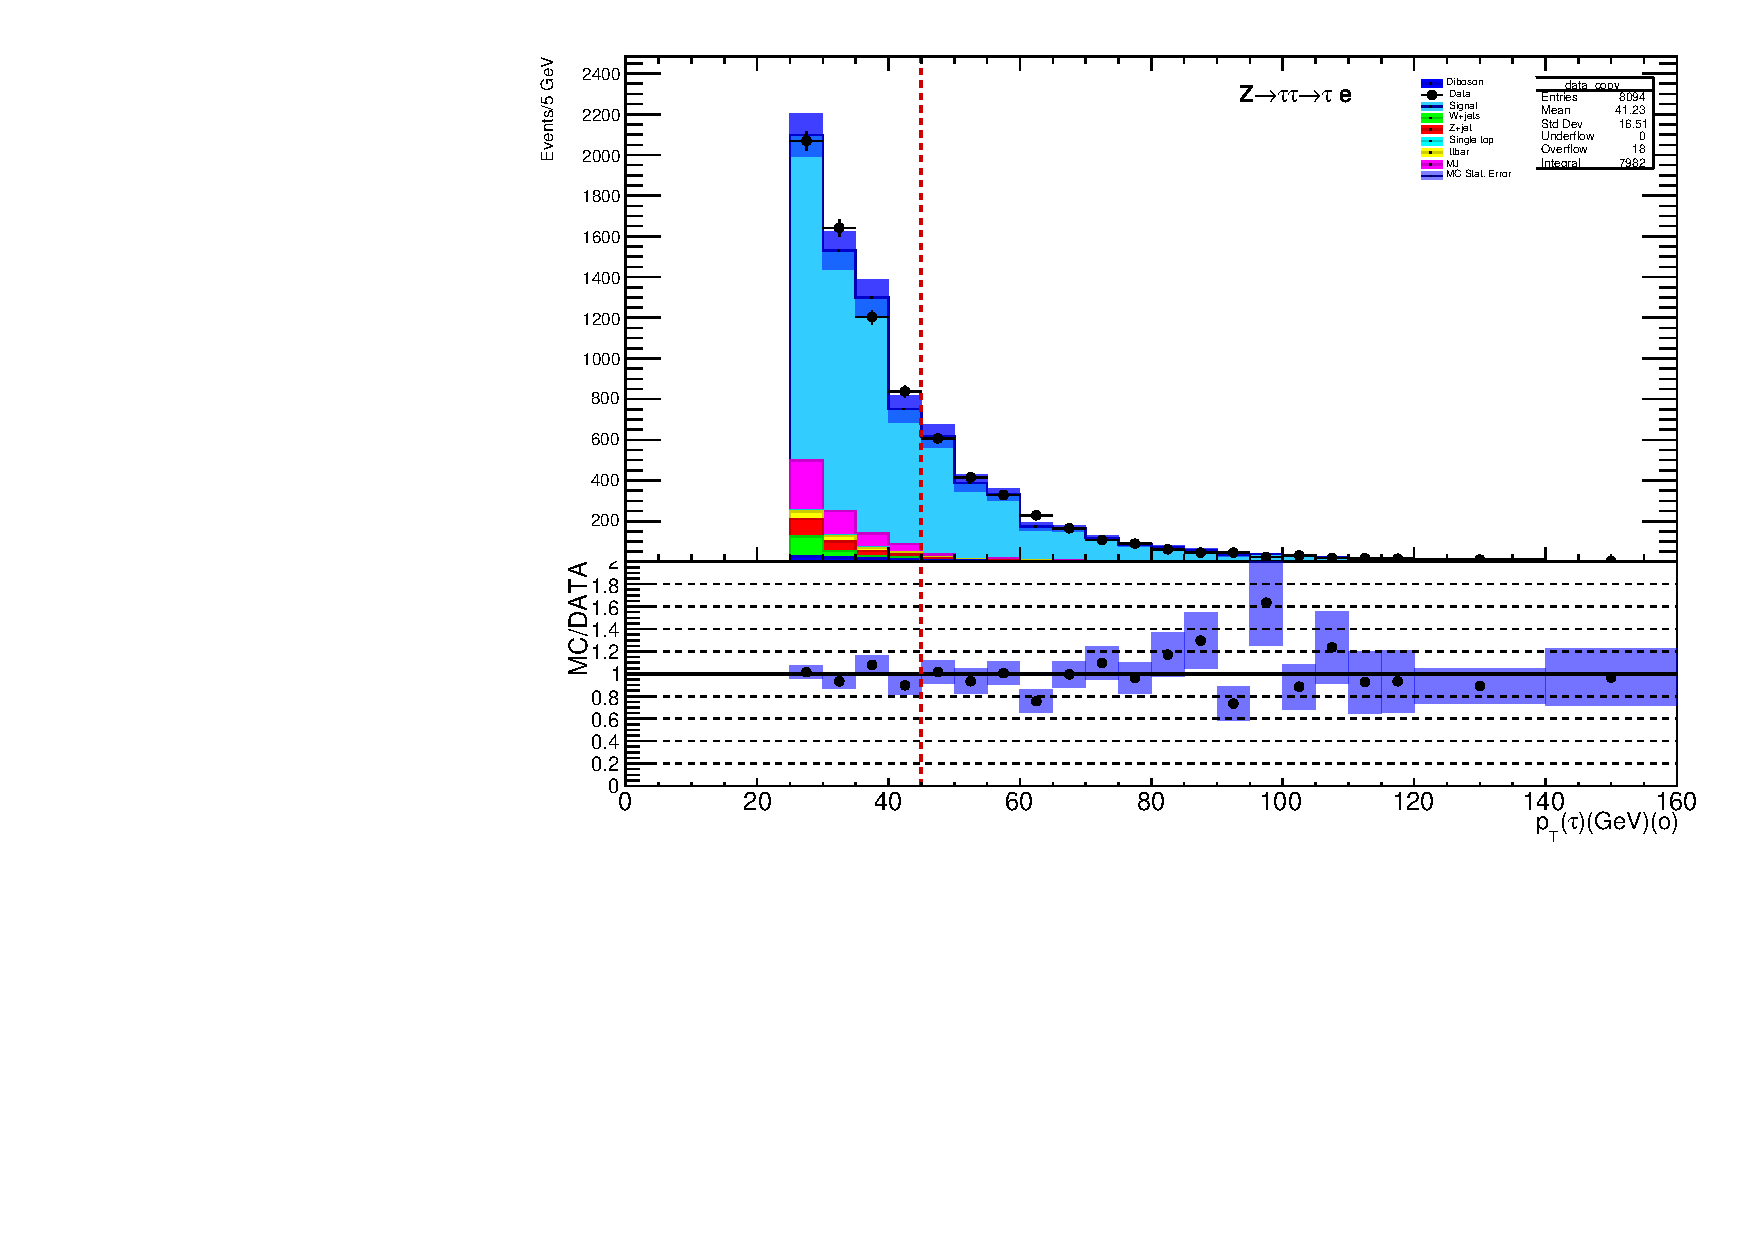
\includegraphics[width=0.50\textwidth]{figures/Fig18i}}}\hfill
	\subfloat[]{\label{Fig18j}{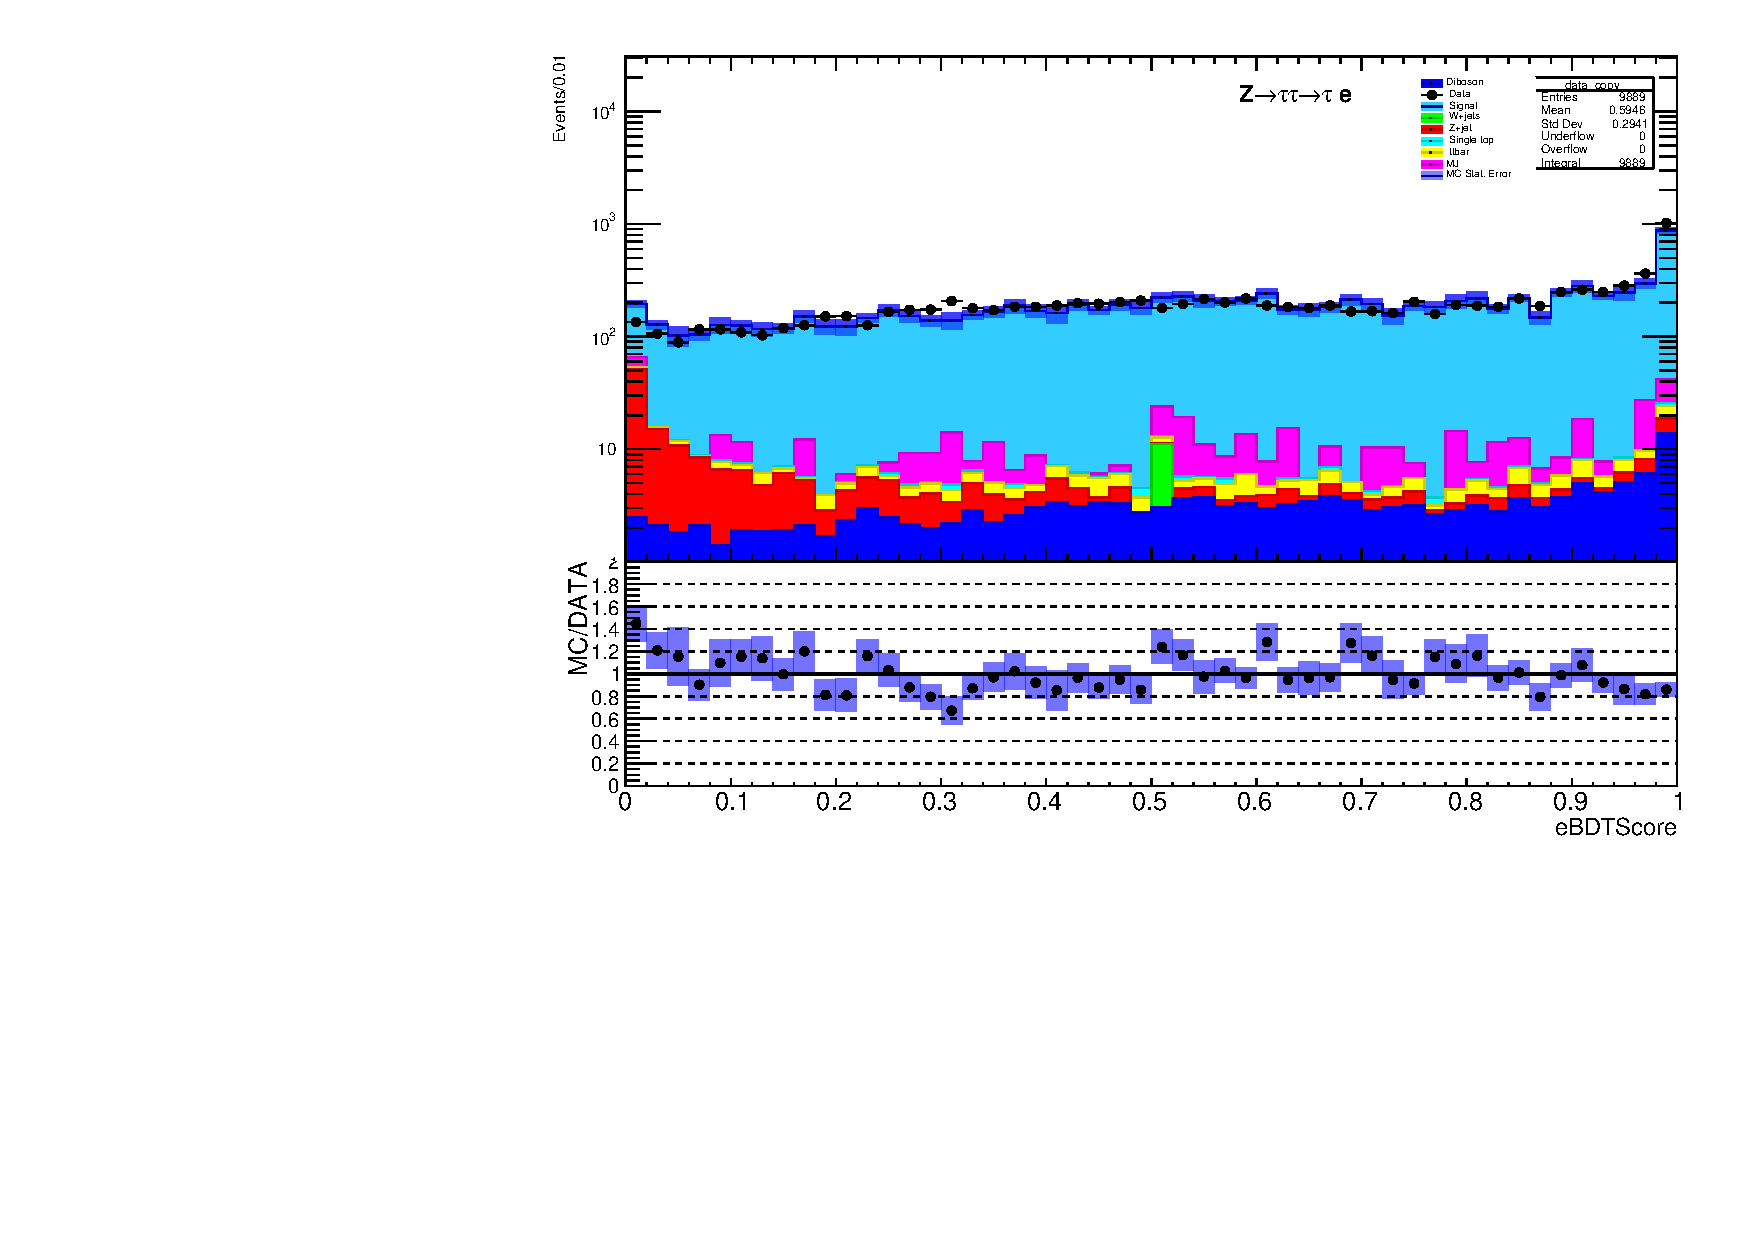
\includegraphics[width=0.50\textwidth]{figures/Fig18j}}}\hfill
	\subfloat[]{\label{Fig18k}{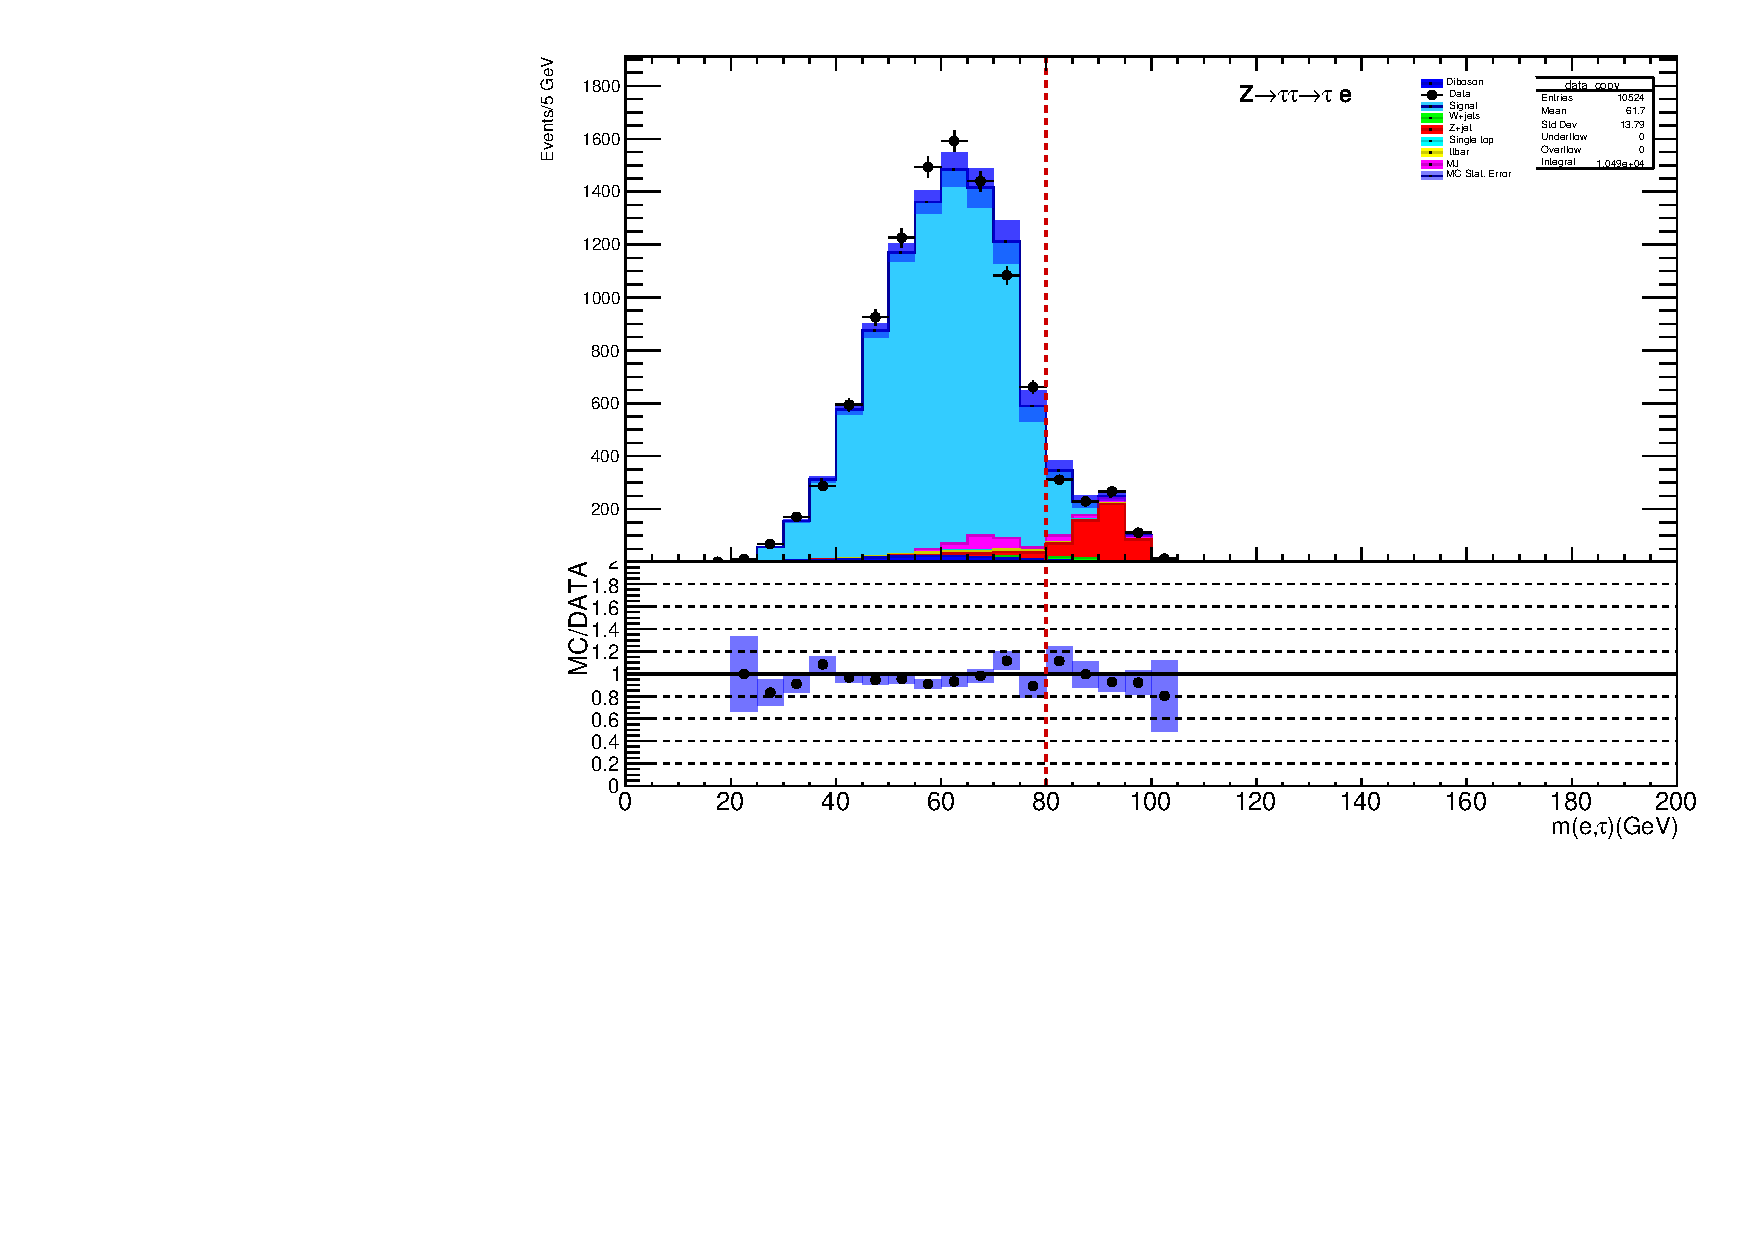
\includegraphics[width=0.50\textwidth]{figures/Fig18k}}}
	\caption{$\mreco$ distribution for the in between region (a) and the outside region (b). All the other cuts have been applied apart from the one being plotted.}
	\label{Fig18}
\end{figure}
    %\input{chapters/7-acknowledgments}
    % If you want a list of your ToDos at the end of the document
    % don't forget to remove before submission!
    %% place it somewhere in the document
\chapter*{ToDo Counters}
\newcounter{ct}%
To Dos: \arabic{todos}; \hspace{1em}%
\setcounter{ct}{0}%
\whiledo {\value{ct} < \value{todos}}%
{%
	\stepcounter {ct}%
    \ref{todo \thect}%
	\ifnum\value{ct} = \value{todos}{}\else{, }\fi
}

Parts to extend: \arabic{extends}; \hspace{1em}%
\setcounter{ct}{0}%
\whiledo {\value{ct} < \value{extends}}%
{%
	\stepcounter {ct}%
	\ref{extend \thect}%
	\ifnum\value{ct} = \value{extends}{}\else{, }\fi
}

Draft parts: \arabic{drafts}; \hspace{1em}%
\setcounter{ct}{0}%
\whiledo {\value{ct} < \value{drafts}}%
{%
	\stepcounter {ct}%
	\ref{draft \thect}%
	\ifnum\value{ct} = \value{drafts}{}\else{, }\fi
}


    \bibliographystyle{abbrv}
    \bibliography{bib/topic1}
    % bibliography is not in the table of contents per default, add it manually
    % enable the \renewcommand for german header
    % \renewcommand{\bibname}{Literaturverzeichnis}
    \addcontentsline{toc}{chapter}{Bibliography}
    \newpage
    \thispagestyle{empty}
    \mbox{}


\end{document}
